%==============================================================================
% Praca dyplomowa (UR) — plik główny
%==============================================================================

\documentclass{urdpl}

%------------------------------------------------------------------------------
% JĘZYK / KODOWANIE (pdfLaTeX)
%------------------------------------------------------------------------------
\usepackage[main=polish,english]{babel}
\usepackage[utf8]{inputenc} % tylko pdfLaTeX

%------------------------------------------------------------------------------
% MATEMATYKA
%------------------------------------------------------------------------------
\usepackage{mathtools}
\usepackage{amssymb}

%------------------------------------------------------------------------------
% HYPERLINKI
%------------------------------------------------------------------------------
\usepackage[hidelinks]{hyperref}

%------------------------------------------------------------------------------
% FLOATY (tylko jeśli używasz [H])
%------------------------------------------------------------------------------
\usepackage{float}

%------------------------------------------------------------------------------
% TABELE (wg potrzeby)
%------------------------------------------------------------------------------
\usepackage{booktabs}
\usepackage{multirow}
\usepackage{tabularx}
\usepackage{array}
\usepackage{makecell}
\usepackage[flushleft]{threeparttable}

\usepackage{xltabular}
\usepackage{ragged2e}

\usepackage{seqsplit}
\usepackage{caption}

\newcommand{\code}[1]{{\ttfamily\seqsplit{#1}}}

\newcolumntype{C}[1]{>{\hsize=#1\hsize\centering\arraybackslash}X}

%------------------------------------------------------------------------------
% OBRAZY
%------------------------------------------------------------------------------

\usepackage{tikz}
\usetikzlibrary{positioning, arrows.meta}

%------------------------------------------------------------------------------
% LISTINGI
%------------------------------------------------------------------------------
\usepackage{listings}
\usepackage{xcolor}

\renewcommand{\lstlistlistingname}{Spis listingów}
\renewcommand{\lstlistingname}{Listing}
\providecommand{\listingname}{\lstlistingname} % alias do odwołań w tekście

\definecolor{codegreen}{rgb}{0,0.6,0}
\definecolor{codegray}{rgb}{0.5,0.5,0.5}

\lstdefinestyle{mystyle}{
  basicstyle=\ttfamily\footnotesize,
  breaklines=true,
  numbers=left,
  numberstyle=\tiny\color{codegray},
  numbersep=6pt,
  showstringspaces=false,
  tabsize=2,
  keywordstyle=\color{blue},
  commentstyle=\color{codegreen},
  stringstyle=\color{red},
  literate={ą}{{\k{a}}}1 {ć}{{\'c}}1 {ę}{{\k{e}}}1 {ó}{{\'o}}1 {ń}{{\'n}}1 {ł}{{\l{}}}1 {ś}{{\'s}}1 {ź}{{\'z}}1 {ż}{{\.z}}1
           {Ą}{{\k{A}}}1 {Ć}{{\'C}}1 {Ę}{{\k{E}}}1 {Ó}{{\'O}}1 {Ń}{{\'N}}1 {Ł}{{\L{}}}1 {Ś}{{\'S}}1 {Ź}{{\'Z}}1 {Ż}{{\.Z}}1
}
\lstset{style=mystyle}



\lstdefinestyle{matlabStyle}{
    language=Matlab,
    basicstyle=\ttfamily\small,
    keywordstyle=\color{blue}\bfseries,
    commentstyle=\color{green!50!black},
    stringstyle=\color{red},
    numbers=left,
    numberstyle=\tiny\color{gray},
    stepnumber=1,
    numbersep=10pt,
    % backgroundcolor=\color{gray!10},
    % frame=single,
    breaklines=true,
    showstringspaces=false,
    tabsize=4
}
%------------------------------------------------------------------------------
% PODKREŚLANIE + NUMERY LINII (opcjonalnie)
%------------------------------------------------------------------------------
\usepackage[normalem]{ulem}
\usepackage{lineno}

%------------------------------------------------------------------------------
% CYTOWANIA
%------------------------------------------------------------------------------
\usepackage{csquotes}

%------------------------------------------------------------------------------
% Nazwy podpisów (opcjonalnie; zwykle babel i klasa wystarczą)
%------------------------------------------------------------------------------
\AtBeginDocument{
  \renewcommand{\tablename}{Tabela}
  \renewcommand{\figurename}{Rys.}
}

%------------------------------------------------------------------------------
% METADANE PRACY (dla urdpl.cls)
%------------------------------------------------------------------------------
\author{Filip Lisowski, Konrad Fugiel}
\shortauthor{F. Lisowski, K. Fugiel}
\noAlbum{134942, 134909}

\titlePL{Dokumentacja projektowa - Wewnętrzny system identyfikacji osób}
\titleEN{Internal Person Identification System}

\shorttitlePL{IdentityCore}
\shorttitleEN{IdentityCore}

\thesistype{Dokumentacja projektowa}
\thesisDone{Prowadzący przedmiotu: }
\supervisor{mgr inż. Ewa Żesławska}

\degreeprogramme{Informatyka}

\date{2026}

\department{Instytut Informatyki}
\faculty{Wydział Nauk Ścisłych i Technicznych}


%------------------------------------------------------------------------------
% NUMERACJA
%------------------------------------------------------------------------------
\setlength{\cftsecnumwidth}{10mm}
\setcounter{secnumdepth}{4}
\setcounter{tocdepth}{2}
\brokenpenalty=10000\relax

%==============================================================================
\begin{document}
%==============================================================================


%------------------------------------------------------------------------------
% Strona tytułowa + podziękowania
%------------------------------------------------------------------------------
\titlepages

% (opcjonalnie) styl plain bez numerów na stronach typu plain
\fancypagestyle{plain}{
  \fancyhf{}
  \renewcommand{\headrulewidth}{0pt}
  \renewcommand{\footrulewidth}{0pt}
}

%------------------------------------------------------------------------------
% Streszczenie (PL) – NIE dodajemy do spisu treści
%------------------------------------------------------------------------------
 
\cleardoublepage
\selectlanguage{polish}
\chapter*{Streszczenie}
\label{cha:streszczenie-pl}

Praca przedstawia projekt i implementację aplikacji \textit{IdentityCore}, będącej lokalnym systemem identyfikacji osób na podstawie danych biometrycznych. System został przygotowany jako aplikacja desktopowa w technologii WPF/.NET, współpracująca z lokalną bazą danych SQL Server. Głównym celem projektu było stworzenie prototypu umożliwiającego prowadzenie rejestru osób, zapisywanie danych biometrycznych, wykonywanie prób identyfikacji oraz analizę uzyskanych wyników.

\bigskip

W projekcie zastosowano dwa rodzaje biometrii: identyfikację twarzy oraz identyfikację odcisku palca. Moduł twarzy wykorzystuje model \texttt{arcface.onnx} do uzyskania reprezentacji cech twarzy, a następnie porównuje ją z zapisanymi wzorcami. Moduł odcisku palca wykorzystuje bibliotekę SourceAFIS do tworzenia i porównywania szablonów biometrycznych. Aplikacja uwzględnia również progi decyzyjne oraz margines pomiędzy najlepszym i drugim kandydatem, co pozwala odrzucać przypadki o zbyt niskim lub niejednoznacznym wyniku.

\bigskip

W ramach projektu przygotowano interfejs użytkownika obejmujący logowanie operatora, panel główny, rejestr osób, widoki identyfikacji twarzy i odcisku palca, historię prób oraz ustawienia systemowe. Przeprowadzone testy potwierdziły działanie podstawowych scenariuszy: poprawnego dopasowania oraz braku dopasowania dla obu typów biometrii. Wyniki mają charakter demonstracyjny i nie stanowią pełnej statystycznej walidacji systemu. Projekt pokazuje jednak kompletny przepływ działania prototypu systemu biometrycznego oraz wskazuje możliwe kierunki dalszego rozwoju, w tym zwiększenie bezpieczeństwa, rozszerzenie testów i dodanie mechanizmów wykrywania żywotności próbki.

%------------------------------------------------------------------------------
% Abstract (EN) – NIE dodajemy do spisu treści
%------------------------------------------------------------------------------
 
\cleardoublepage
\selectlanguage{english}
\chapter*{Abstract}
\label{cha:abstract-en}

This project presents the design and implementation of \textit{IdentityCore}, a local biometric identification system for persons. The system was developed as a desktop application using WPF/.NET and a local SQL Server database. The main objective of the project was to create a prototype that supports person registration, biometric data management, identification attempts, result presentation and identification history analysis.

\bigskip

The application uses two biometric modalities: face identification and fingerprint identification. The face module uses the \texttt{arcface.onnx} model to generate a numerical representation of facial features, which is then compared with previously stored templates. The fingerprint module uses the SourceAFIS library to create and compare biometric fingerprint templates. The system also applies decision thresholds and a margin between the best and the second-best candidate, allowing uncertain or low-quality matches to be rejected.

\bigskip

The project includes a user interface with operator login, dashboard, person registry, face identification view, fingerprint identification view, identification history and system settings. The performed tests confirmed the operation of the basic scenarios: successful matching and no-match decisions for both biometric modules. The results should be treated as a demonstration of a prototype rather than a full statistical validation of a biometric system. Nevertheless, the project demonstrates a complete workflow of a biometric identification application and indicates possible directions for further development, including improved security, extended testing and the introduction of liveness detection mechanisms.

%------------------------------------------------------------------------------
% Spis treści
%------------------------------------------------------------------------------

\cleardoublepage
\selectlanguage{polish}
\tableofcontents

\clearpage
% \linenumbers % jeśli nie chcesz numerów linii w całości, usuń lub przenieś

%------------------------------------------------------------------------------
% Rozdziały
%------------------------------------------------------------------------------
\chapter{Wprowadzenie}
\label{chap:wprowadzenie}

\section{Kontekst projektu}

Systemy identyfikacji osób są wykorzystywane wszędzie tam, gdzie konieczne jest powiązanie danych zapisanych w systemie z konkretną osobą. W typowych rozwiązaniach informatycznych identyfikacja może opierać się na loginie, haśle, karcie dostępu lub numerze ewidencyjnym. Takie metody są proste w użyciu, ale nie zawsze potwierdzają fizyczną obecność właściwej osoby. Z tego powodu w systemach bezpieczeństwa coraz częściej wykorzystuje się dane biometryczne, czyli cechy bezpośrednio związane z człowiekiem.

Projekt \textit{IdentityCore} dotyczy aplikacji służącej do wewnętrznej identyfikacji osób z wykorzystaniem dwóch cech biometrycznych: twarzy oraz odcisku palca. System został przygotowany jako aplikacja lokalna, której zadaniem jest obsługa rejestru osób, danych biometrycznych oraz prób identyfikacji. Przyjęty scenariusz odpowiada uproszczonemu systemowi wykorzystywanemu w środowisku demonstracyjnym lub laboratoryjnym, w którym operator może zarządzać profilami osób i sprawdzać wyniki identyfikacji.

Projekt nie jest gotowym systemem produkcyjnym przeznaczonym do pracy w środowisku wysokiego ryzyka, ale pozwala zaprezentować pełny przebieg tworzenia aplikacji łączącej część użytkową, bazodanową oraz biometryczną.

\section{Cel projektu}

Głównym celem projektu było zaprojektowanie i wykonanie aplikacji \textit{IdentityCore}, która umożliwia identyfikację osób na podstawie danych biometrycznych. Aplikacja ma pozwalać na zapis danych osoby, powiązanie ich z próbkami biometrycznymi, wykonanie próby identyfikacji oraz zaprezentowanie wyniku w czytelnej formie.

Cel projektu obejmuje dwa uzupełniające się obszary. Pierwszy z nich dotyczy części biometrycznej, czyli wykorzystania obrazów twarzy i odcisków palców do rozpoznawania osób. Drugi dotyczy części aplikacyjnej, obejmującej zaprojektowanie kompletnego programu desktopowego z interfejsem użytkownika, bazą danych, obsługą logowania, historią działań oraz uporządkowaną strukturą kodu.

W efekcie projekt ma pokazać nie tylko samą ideę identyfikacji biometrycznej, ale również sposób jej osadzenia w działającej aplikacji użytkowej.

\section{Zakres projektu}

Zakres projektu obejmuje przygotowanie aplikacji umożliwiającej podstawową obsługę procesu wewnętrznej identyfikacji osób. W ramach systemu przewidziano następujące obszary funkcjonalne:
\begin{itemize}
    \item dostęp do aplikacji poprzez ekran logowania,
    \item prowadzenie rejestru osób,
    \item obsługę danych opisowych i zdjęcia profilowego osoby,
    \item zapis i wykorzystanie danych biometrycznych twarzy,
    \item zapis i wykorzystanie danych biometrycznych odcisku palca,
    \item wykonanie próby identyfikacji osoby,
    \item prezentację wyniku identyfikacji,
    \item zapis historii wykonanych prób,
    \item konfigurację parametrów wpływających na decyzję systemu.
\end{itemize}

\section{Charakter projektu łączonego}

Dokumentacja opisuje jeden spójny projekt realizowany na potrzeby dwóch przedmiotów: \textit{Biometryczne Systemy Zabezpieczeń} oraz \textit{Programowanie Obiektowe II}. Z tego powodu aplikacja została opracowana tak, aby łączyć wymagania związane z analizą danych biometrycznych oraz wymagania dotyczące tworzenia aplikacji obiektowej.

Część związana z biometrią koncentruje się na wykorzystaniu danych twarzy i odcisku palca w procesie identyfikacji osoby. Obejmuje ona przygotowanie danych wejściowych, utworzenie reprezentacji biometrycznej, porównanie z danymi zapisanymi w systemie oraz interpretację wyniku.

Część związana z programowaniem obiektowym obejmuje zaprojektowanie aplikacji desktopowej, podział projektu na logiczne moduły, komunikację z bazą danych, obsługę interfejsu użytkownika, walidację danych oraz zapis historii działania systemu.

Takie połączenie pozwala traktować \textit{IdentityCore} jako kompletną aplikację, w której mechanizmy biometryczne nie są oderwanym eksperymentem, lecz częścią większego systemu użytkowego.
\chapter{Analiza problemu i istniejących rozwiązań}
\label{chap:analiza-problemu}

\section{Opis problemu}

Identyfikacja osoby w systemie informatycznym polega na ustaleniu, kto korzysta z systemu lub do kogo należy analizowany zestaw danych. W wielu aplikacjach proces ten opiera się na klasycznych metodach, takich jak login, hasło, karta dostępu, numer identyfikacyjny albo ręczna weryfikacja danych przez operatora. Rozwiązania te są powszechnie stosowane, ale w systemach bezpieczeństwa mogą być niewystarczające.

Hasło może zostać zapomniane, ujawnione lub przechwycone. Karta dostępowa może zostać zgubiona albo przekazana innej osobie. Ręczna weryfikacja danych zależy natomiast od dokładności operatora i może być czasochłonna przy większej liczbie osób. W takich przypadkach sam identyfikator nie zawsze potwierdza, że dana osoba rzeczywiście jest tą, za którą się podaje.

Cechy biometryczne mogą wspierać ten proces, ponieważ są powiązane bezpośrednio z człowiekiem. Twarz i odcisk palca należą do najczęściej wykorzystywanych cech tego typu. Mogą zostać zarejestrowane w postaci obrazu, przetworzone do reprezentacji biometrycznej, a następnie porównane z danymi zapisanymi wcześniej w systemie. Dzięki temu identyfikacja nie opiera się wyłącznie na wiedzy użytkownika lub posiadanym nośniku, ale także na analizie cechy fizycznej.

W projekcie analizowany problem dotyczy identyfikacji osoby na podstawie wcześniej zarejestrowanych danych biometrycznych. System porównuje nową próbkę z danymi zapisanymi w bazie i wskazuje, czy odnaleziono dopasowanie.

\section{Dane biometryczne wykorzystywane w projekcie}

W projekcie wykorzystywane są dwa typy danych biometrycznych:
\begin{itemize}
    \item obraz twarzy,
    \item obraz odcisku palca.
\end{itemize}

Obraz twarzy stanowi dane wejściowe pozwalające na utworzenie reprezentacji osoby na podstawie jej cech wyglądu. Tego typu dane mogą pochodzić z pliku graficznego lub z kamery. Dla poprawnego działania systemu ważne jest, aby twarz była widoczna, odpowiednio oświetlona i możliwa do przetworzenia.

Obraz odcisku palca jest drugim rodzajem danych wejściowych. W tym przypadku system wykorzystuje plik graficzny przedstawiający układ linii papilarnych. Obraz taki służy do utworzenia reprezentacji biometrycznej odcisku, która może zostać porównana z wcześniej zapisanymi danymi.

Oba typy danych nie są traktowane jako zwykłe obrazy porównywane bezpośrednio piksel po pikselu. Ich rola polega na dostarczeniu informacji potrzebnych do utworzenia reprezentacji biometrycznej, która następnie może zostać wykorzystana w procesie identyfikacji. Szczegóły sposobu tworzenia i porównywania tych reprezentacji opisano w dalszym rozdziale dotyczącym metod i algorytmów.

\newpage

\section{Założenia i ograniczenia systemu}

Przyjęto, że system nie pełni roli produkcyjnego systemu bezpieczeństwa, lecz służy do zaprezentowania procesu identyfikacji osób na podstawie danych biometrycznych.

Najważniejsze założenia przyjęte w projekcie są następujące:
\begin{itemize}
    \item system jest obsługiwany przez operatora,
    \item identyfikacja odbywa się na podstawie danych wcześniej zapisanych w bazie,
    \item analizowane dane mają postać obrazów twarzy i odcisków palców,
    \item skuteczność identyfikacji zależy od jakości danych wejściowych,
    \item wynik systemu ma wspierać proces identyfikacji, a nie zastępować pełnej ekspertyzy biometrycznej.
\end{itemize}

Na działanie systemu wpływa jakość obrazu. W przypadku twarzy znaczenie mają między innymi oświetlenie, ostrość zdjęcia, kąt ustawienia głowy oraz zasłonięcie części twarzy. W przypadku odcisku palca istotne są kompletność odcisku, jakość skanu, położenie palca oraz widoczność charakterystycznych elementów linii papilarnych.

Istotnym ograniczeniem jest również brak pełnej detekcji żywotności użytkownika. System analizuje dostarczony obraz, ale nie potwierdza, czy próbka pochodzi od żywej osoby obecnej w momencie identyfikacji.

Możliwym skutkiem ograniczeń jakościowych jest błędna identyfikacja albo odrzucenie poprawnej osoby. Szczegółowa analiza takich zagrożeń oraz odporności systemu została wydzielona do rozdziału poświęconego bezpieczeństwu.

\section{Analiza istniejących rozwiązań}

\subsection{Windows Hello}

Windows Hello jest mechanizmem uwierzytelniania użytkownika w systemie Windows. Może wykorzystywać między innymi rozpoznawanie twarzy, odcisk palca lub kod PIN \cite{windowshello}. Rozwiązanie to jest stosowane głównie do logowania do urządzenia oraz potwierdzania tożsamości użytkownika w środowisku systemu operacyjnego.

Zaletą Windows Hello jest wygoda użytkowania i integracja z systemem Windows. Użytkownik nie musi za każdym razem wpisywać hasła, a proces uwierzytelniania odbywa się szybko i lokalnie na urządzeniu. Ograniczeniem z perspektywy projektu jest zamknięty charakter rozwiązania. Użytkownik nie ma pełnego wglądu w sposób przetwarzania danych biometrycznych, strukturę zapisanych reprezentacji ani szczegóły podejmowania decyzji.

W odniesieniu do projektu IdentityCore Windows Hello stanowi przykład praktycznego wykorzystania biometrii w aplikacjach codziennego użytku. Różnica polega na tym, że IdentityCore nie jest mechanizmem logowania do systemu operacyjnego, lecz aplikacją demonstracyjną pozwalającą obserwować cały proces zarządzania osobami i próbami identyfikacji.

\newpage

\subsection{Face ID}

Face ID jest systemem rozpoznawania twarzy stosowanym w urządzeniach firmy Apple \cite{faceid}. Jego głównym zadaniem jest odblokowywanie urządzenia, autoryzacja operacji oraz potwierdzanie tożsamości użytkownika w ramach ekosystemu Apple. System wykorzystuje biometrię twarzy i jest zintegrowany bezpośrednio ze sprzętem oraz oprogramowaniem urządzenia.

Najważniejszą zaletą Face ID jest wygoda i wysoki poziom integracji z urządzeniem. Proces uwierzytelniania jest szybki, a użytkownik nie musi wykonywać dodatkowych czynności poza spojrzeniem na urządzenie. Ograniczeniem z punktu widzenia dokumentowanego projektu jest to, że Face ID działa jako zamknięty mechanizm systemowy. Nie jest rozwiązaniem służącym do prowadzenia własnego rejestru osób, analizy historii prób ani eksperymentowania z parametrami działania.

Dla projektu IdentityCore Face ID jest punktem odniesienia w zakresie wykorzystania twarzy jako cechy biometrycznej. Projekt nie próbuje odtwarzać tak zaawansowanego systemu sprzętowo-programowego, lecz pokazuje uproszczony proces identyfikacji twarzy w aplikacji desktopowej.

\subsection{Systemy kontroli dostępu z odciskiem palca}

Systemy kontroli dostępu wykorzystujące odciski palców są stosowane między innymi w firmach, laboratoriach, zamkach elektronicznych oraz systemach ewidencji czasu pracy. Ich zadaniem jest sprawdzenie, czy osoba przykładająca palec do czytnika znajduje się w bazie uprawnionych użytkowników \cite{fingerprintaccess}.

Zaletą takich systemów jest prostota użycia oraz bezpośrednie powiązanie próby dostępu z cechą fizyczną użytkownika. Odcisk palca jest wygodny w codziennym użyciu i może być szybko porównany z zapisanymi wzorcami. Ograniczenia dotyczą przede wszystkim jakości odczytu, zabrudzenia palca lub skanera, nieprawidłowego przyłożenia palca oraz ryzyka użycia sztucznie przygotowanego odcisku.

W porównaniu z takimi rozwiązaniami IdentityCore nie jest terminalem kontroli dostępu. Aplikacja nie otwiera drzwi ani nie zarządza uprawnieniami fizycznymi. Wykorzystuje jednak podobny typ danych biometrycznych i pozwala przeanalizować proces identyfikacji odcisku w środowisku projektowym.

\subsection{Komercyjne SDK i systemy biometryczne}

Istnieją również komercyjne zestawy SDK oraz systemy biometryczne umożliwiające budowę aplikacji wykorzystujących rozpoznawanie twarzy, odcisków palców lub innych cech biometrycznych \cite{biometricsdk}. Tego typu rozwiązania oferują gotowe mechanizmy obsługi danych biometrycznych, porównywania próbek, a czasem również integrację z urządzeniami zewnętrznymi.

Ich zaletą jest szeroki zakres funkcji oraz możliwość użycia w profesjonalnych systemach bezpieczeństwa. Ograniczeniem w kontekście projektu jest często zamknięty charakter bibliotek oraz mniejsza przejrzystość działania. Część procesu rozpoznawania pozostaje ukryta wewnątrz gotowego narzędzia.

IdentityCore korzysta z gotowych narzędzi jedynie tam, gdzie jest to uzasadnione zakresem projektu, ale samodzielnie organizuje przepływ danych, rejestr osób, zapis prób i prezentację wyników. Dzięki temu aplikacja pozwala lepiej pokazać zależność między jakością danych, sposobem ich porównania i decyzją systemu.

\newpage

\section{Wyróżniki projektowanego rozwiązania}

IdentityCore różni się od opisanych rozwiązań przede wszystkim tym, że łączy kilka elementów w jednej aplikacji desktopowej. System nie jest wyłącznie mechanizmem logowania ani terminalem kontroli dostępu, lecz aplikacją pozwalającą zarządzać osobami, próbkami biometrycznymi oraz wynikami prób identyfikacji.

Najważniejsze wyróżniki projektowanego rozwiązania to:
\begin{itemize}
    \item połączenie identyfikacji twarzy i odcisku palca w jednej aplikacji,
    \item możliwość zarządzania osobami i próbkami biometrycznymi,
    \item zapis historii prób identyfikacji,
    \item możliwość późniejszej analizy skuteczności działania systemu.
\end{itemize}

Projekt nie konkuruje z komercyjnymi systemami biometrycznymi pod względem poziomu zabezpieczeń ani gotowości produkcyjnej. Jego wartość polega na pokazaniu kompletnego procesu identyfikacji w aplikacji, która łączy część biometryczną, użytkową i analityczną.

\chapter{Wymagania systemowe}
\label{chap:wymagania-systemowe}

\section{Wymagania funkcjonalne}

Wymagania funkcjonalne określają funkcje, które system powinien udostępniać operatorowi. W przypadku aplikacji \textit{IdentityCore} dotyczą one przede wszystkim obsługi rejestru osób, danych biometrycznych, procesu identyfikacji oraz historii wykonanych prób.

\renewcommand{\arraystretch}{1.15}
\begin{xltabular}{\textwidth}{|
    >{\RaggedRight\arraybackslash}p{1.5cm}|
    >{\RaggedRight\arraybackslash}p{3.2cm}|
    >{\RaggedRight\arraybackslash}X|
    >{\RaggedRight\arraybackslash}p{1.8cm}|}
    
    \hline
    \textbf{Id} & \textbf{Nazwa wymagania} & \textbf{Opis wymagania} & \textbf{Priorytet} \\
    \hline
    \endfirsthead

    \hline
    \textbf{Id} & \textbf{Nazwa wymagania} & \textbf{Opis wymagania} & \textbf{Priorytet} \\
    \hline
    \endhead

    WF-01 & Logowanie operatora & System powinien umożliwiać operatorowi zalogowanie się do aplikacji przed uzyskaniem dostępu do głównych funkcji. & Wysoki \\
    \hline
    WF-02 & Panel główny & System powinien udostępniać panel główny prezentujący podstawowe informacje o stanie danych i ostatnich działaniach. & Średni \\
    \hline
    WF-03 & Rejestr osób & System powinien umożliwiać przeglądanie osób zapisanych w rejestrze. & Wysoki \\
    \hline
    WF-04 & Dodawanie osoby & System powinien umożliwiać dodanie nowej osoby wraz z podstawowymi danymi opisowymi. & Wysoki \\
    \hline
    WF-05 & Edycja danych osoby & System powinien umożliwiać aktualizację danych osoby zapisanej w rejestrze. & Wysoki \\
    \hline
    WF-06 & Zdjęcie profilowe & System powinien umożliwiać przypisanie zdjęcia profilowego do osoby. & Średni \\
    \hline
    WF-07 & Próbki twarzy & System powinien umożliwiać zapis danych biometrycznych twarzy przypisanych do osoby. & Wysoki \\
    \hline
    WF-08 & Próbki odcisku palca & System powinien umożliwiać zapis danych biometrycznych odcisku palca przypisanych do osoby. & Wysoki \\
    \hline
    WF-09 & Identyfikacja twarzy & System powinien umożliwiać wykonanie próby identyfikacji osoby na podstawie obrazu twarzy. & Wysoki \\
    \hline
    WF-10 & Identyfikacja odcisku palca & System powinien umożliwiać wykonanie próby identyfikacji osoby na podstawie obrazu odcisku palca. & Wysoki \\
    \hline
    WF-11 & Prezentacja wyniku & System powinien prezentować wynik identyfikacji w formie informacji o znalezionym dopasowaniu albo jego braku. & Wysoki \\
    \hline
    WF-12 & Historia prób & System powinien umożliwiać zapis informacji o wykonanych próbach identyfikacji. & Wysoki \\
    \hline
    WF-13 & Przeglądanie historii & System powinien umożliwiać przeglądanie i filtrowanie historii prób identyfikacji. & Średni \\
    \hline
    WF-14 & Ustawienia systemowe & System powinien umożliwiać konfigurację wybranych parametrów wpływających na decyzję identyfikacyjną. & Średni \\
    \hline
    WF-15 & Komunikaty systemowe & System powinien informować operatora o podstawowych błędach, brakach danych lub wyniku wykonanej operacji. & Wysoki \\
    \hline

    \caption{Wymagania funkcjonalne systemu}
    \label{tab:wymagania-funkcjonalne} \\
\end{xltabular}

Wymagania funkcjonalne opisują zakres pracy systemu z perspektywy operatora. Nie określają sposobu realizacji poszczególnych funkcji, lecz wskazują, jakie działania powinny być możliwe w gotowej aplikacji.

\section{Wymagania niefunkcjonalne}

Wymagania niefunkcjonalne określają cechy jakościowe systemu. Dotyczą między innymi środowiska pracy, czytelności interfejsu, stabilności działania oraz organizacji projektu.

\renewcommand{\arraystretch}{1.15}
\begin{xltabular}{\textwidth}{|
    >{\RaggedRight\arraybackslash}p{1.5cm}|
    >{\RaggedRight\arraybackslash}p{3.2cm}|
    >{\RaggedRight\arraybackslash}X|
    >{\RaggedRight\arraybackslash}p{1.8cm}|}

    \hline
    \textbf{Id} & \textbf{Nazwa wymagania} & \textbf{Opis wymagania} & \textbf{Priorytet} \\
    \hline
    \endfirsthead

    \hline
    \textbf{Id} & \textbf{Nazwa wymagania} & \textbf{Opis wymagania} & \textbf{Priorytet} \\
    \hline
    \endhead

    WNF-01 & Środowisko Windows & Aplikacja powinna działać w środowisku systemu Windows. & Wysoki \\
    \hline
    WNF-02 & Praca lokalna & System powinien działać lokalnie, bez konieczności korzystania z zewnętrznego serwera. & Wysoki \\
    \hline
    WNF-03 & Baza danych & Dane systemu powinny być przechowywane w lokalnej relacyjnej bazie danych. & Wysoki \\
    \hline
    WNF-04 & Czytelność interfejsu & Interfejs użytkownika powinien być spójny, czytelny i dostosowany do obsługi. & Wysoki \\
    \hline
    WNF-05 & Stabilność działania & System powinien obsługiwać typowe sytuacje błędne bez przerywania pracy aplikacji. & Wysoki \\
    \hline
    WNF-06 & Obsługa błędów & Komunikaty błędów powinny być zrozumiałe i wskazywać przyczynę problemu. & Wysoki \\
    \hline
    WNF-07 & Uporządkowanie danych & Dane osób, próbek biometrycznych, ustawień i historii prób powinny być przechowywane w uporządkowanej strukturze. & Wysoki \\
    \hline
    WNF-08 & Przejrzystość kodu & Kod aplikacji powinien być podzielony zgodnie z odpowiedzialnością poszczególnych elementów systemu. & Średni \\
    \hline

    \caption{Wymagania niefunkcjonalne systemu}
    \label{tab:wymagania-niefunkcjonalne}
\end{xltabular}

Wymagania niefunkcjonalne są istotne, ponieważ projekt nie ogranicza się do samego działania funkcji. Aplikacja powinna być możliwa do uruchomienia, czytelna w obsłudze i odporna na podstawowe błędy użytkownika.

\section{Wymagania dotyczące bezpieczeństwa}

Wymagania dotyczące bezpieczeństwa określają podstawowe oczekiwania związane z kontrolą dostępu, przechowywaniem danych oraz ograniczaniem ryzyka błędnej interpretacji wyniku. Szczegółowa analiza zagrożeń została przedstawiona w osobnym rozdziale, dlatego w tym miejscu wskazano jedynie wymagania systemowe.

\renewcommand{\arraystretch}{1.15}
\begin{xltabular}{\textwidth}{|
    >{\RaggedRight\arraybackslash}p{1.5cm}|
    >{\RaggedRight\arraybackslash}p{3.2cm}|
    >{\RaggedRight\arraybackslash}X|
    >{\RaggedRight\arraybackslash}p{1.8cm}|}

    \hline
    \textbf{Id} & \textbf{Nazwa wymagania} & \textbf{Opis wymagania} & \textbf{Priorytet} \\
    \hline
    \endfirsthead

    \hline
    \textbf{Id} & \textbf{Nazwa wymagania} & \textbf{Opis wymagania} & \textbf{Priorytet} \\
    \hline
    \endhead

    WB-01 & Kontrola dostępu & Dostęp do głównych funkcji aplikacji powinien być poprzedzony logowaniem operatora. & Wysoki \\
    \hline
    WB-02 & Dane osób & System powinien przechowywać dane osób w bazie danych w sposób uporządkowany i powiązany z właściwym profilem. & Wysoki \\
    \hline
    WB-03 & Dane biometryczne & Dane biometryczne powinny być przypisywane do odpowiedniej osoby zapisanej w rejestrze. & Wysoki \\
    \hline
    WB-04 & Historia prób & System powinien zapisywać informacje o wykonanych próbach identyfikacji, aby możliwa była późniejsza analiza działania systemu. & Wysoki \\
    \hline
    WB-05 & Parametry decyzyjne & System powinien umożliwiać kontrolę parametrów wpływających na decyzję identyfikacyjną. & Średni \\
    \hline
    WB-06 & Ograniczenie błędnej identyfikacji & System powinien uwzględniać mechanizmy ograniczające ryzyko przypadkowego wskazania niewłaściwej osoby. & Wysoki \\
    \hline
    WB-07 & Informowanie o wyniku & System powinien jednoznacznie informować operatora, czy dopasowanie zostało znalezione, czy nie. & Wysoki \\
    \hline
    WB-08 & Błędne dane wejściowe & System powinien reagować na podstawowe problemy z danymi wejściowymi, takie jak brak pliku, nieczytelny obraz lub brak danych porównawczych. & Wysoki \\
    \hline

    \caption{Wymagania dotyczące bezpieczeństwa}
    \label{tab:wymagania-bezpieczenstwa}
\end{xltabular}

Wymagania bezpieczeństwa w tym rozdziale mają charakter podstawowy. Nie oznaczają, że system spełnia wymagania produkcyjnego systemu ochrony dostępu. Ich celem jest wskazanie, jakie mechanizmy powinny ograniczać błędne użycie aplikacji w warunkach projektowych.

\newpage

\section{Założenia dotyczące użytkowników i środowiska pracy}

System został zaprojektowany z myślą o obsłudze przez operatora. Operator korzysta z aplikacji lokalnie, zarządza danymi osób, uruchamia próby identyfikacji i analizuje ich wyniki. Nie zakłada się rozbudowanego modelu wielu użytkowników, ról ani uprawnień.

Przyjęto następujące założenia dotyczące użytkowników i środowiska pracy:
\begin{itemize}
    \item aplikacja jest obsługiwana przez jednego operatora,
    \item system działa lokalnie na komputerze z systemem Windows,
    \item dane osób muszą zostać wcześniej zapisane w bazie,
    \item identyfikacja odbywa się względem osób już zarejestrowanych w systemie,
    \item skuteczność identyfikacji zależy od jakości dostarczonych danych wejściowych,
    \item projekt jest przeznaczony wyłącznie do prezentacji i testów,
    \item system nie stanowi kompletnego produkcyjnego rozwiązania bezpieczeństwa.
\end{itemize}

Założenia te wyznaczają granice odpowiedzialności systemu. Aplikacja ma umożliwić przeprowadzenie i ocenę procesu identyfikacji biometrycznej w kontrolowanych warunkach, a nie zastępować profesjonalny system kontroli dostępu.
\chapter{Koncepcja rozwiązania biometrycznego}
\label{chap:koncepcja-rozwiazania}

\section{Ogólna idea działania systemu}

Koncepcja systemu \textit{IdentityCore} opiera się na prowadzeniu lokalnego rejestru osób oraz powiązaniu każdej osoby z danymi biometrycznymi. Dane te mogą dotyczyć twarzy lub odcisku palca. Po zapisaniu osoby i jej próbek system może wykonać próbę identyfikacji na podstawie nowej próbki wejściowej.

Identyfikacja odbywa się względem danych już dostępnych w systemie. Oznacza to, że analizowana próbka nie jest oceniana samodzielnie, lecz porównywana z wcześniej zapisanymi reprezentacjami biometrycznymi osób znajdujących się w rejestrze. Wynikiem procesu jest wskazanie najlepszego dopasowania albo informacja, że dopasowanie nie zostało znalezione.

\section{Pipeline przetwarzania danych}

Pipeline systemu biometrycznego opisuje ogólny przepływ danych od momentu dostarczenia próbki wejściowej do uzyskania wyniku identyfikacji. W przypadku obu wykorzystywanych modalności -- twarzy oraz odcisku palca -- proces ma podobną strukturę koncepcyjną: dane wejściowe są przygotowywane do analizy, przekształcane do postaci reprezentacji biometrycznej, a następnie porównywane z danymi zapisanymi wcześniej w systemie.

Na podstawie porównania system wyznacza najlepiej dopasowanego kandydata i podejmuje decyzję, czy wynik można uznać za poprawne dopasowanie. Informacja o wykonanej próbie może zostać zapisana w historii, co umożliwia późniejszą analizę oraz ocenę poprawności przeprowadzonych identyfikacji.

\bigskip

Na rysunku~\ref{fig:pipeline-identitycore} przedstawiono uproszczony przepływ danych od momentu pozyskania próbki wejściowej do zapisania informacji o wykonanej próbie identyfikacji.

\begin{figure}[H]
    \centering
    \begin{tikzpicture}[
        node distance=0.6cm,
        block/.style={
            rectangle,
            draw,
            rounded corners,
            align=center,
            minimum width=9.5cm,
            minimum height=0.75cm,
            font=\small
        },
        arrow/.style={
            -{Latex[length=3mm]},
            thick
        }
    ]

        \node[block] (input) {Pozyskanie danych wejściowych\\obraz twarzy lub obraz odcisku palca};
        \node[block, below=of input] (prep) {Przygotowanie danych do analizy};
        \node[block, below=of prep] (repr) {Utworzenie reprezentacji biometrycznej};
        \node[block, below=of repr] (compare) {Porównanie z zapisanymi wzorcami};
        \node[block, below=of compare] (match) {Wyznaczenie najlepszego dopasowania};
        \node[block, below=of match] (decision) {Podjęcie decyzji o wyniku identyfikacji};
        \node[block, below=of decision] (history) {Zapis informacji o wykonanej próbie};

        \draw[arrow] (input) -- (prep);
        \draw[arrow] (prep) -- (repr);
        \draw[arrow] (repr) -- (compare);
        \draw[arrow] (compare) -- (match);
        \draw[arrow] (match) -- (decision);
        \draw[arrow] (decision) -- (history);

    \end{tikzpicture}
    \caption{Ogólny pipeline działania systemu biometrycznego IdentityCore}
    \label{fig:pipeline-identitycore}
\end{figure}

\newpage

\section{Proces rejestracji osoby}

Proces rejestracji osoby polega na utworzeniu w systemie profilu, który może zostać później wykorzystany podczas identyfikacji. Nie jest to rejestracja konta użytkownika aplikacji, lecz dodanie wpisu osoby do rejestru identyfikacyjnego wraz z przypisanymi danymi opisowymi i biometrycznymi.

W praktyce proces ten obejmuje wprowadzenie podstawowych danych osoby, dodanie zdjęcia profilowego oraz zapisanie próbek biometrycznych twarzy i odcisku palca. Dane opisowe oraz zdjęcie profilowe służą do czytelnej prezentacji osoby w aplikacji, natomiast próbki biometryczne stanowią dane odniesienia wykorzystywane podczas późniejszych prób identyfikacji.

Osoba, dla której nie zapisano danych biometrycznych danego typu, nie może zostać skutecznie zidentyfikowana z użyciem tej modalności. Oznacza to, że jakość i kompletność danych zebranych na etapie rejestracji mają bezpośredni wpływ na późniejszą skuteczność działania systemu.

\bigskip
\bigskip

Na rysunku~\ref{fig:rejestracja-osoby} przedstawiono uproszczony przebieg procesu rejestracji osoby w systemie \textit{IdentityCore}.

\begin{figure}[htbp]
    \centering
    \begin{tikzpicture}[
        node distance=0.55cm,
        block/.style={
            rectangle,
            draw,
            rounded corners,
            align=center,
            minimum width=7.2cm,
            minimum height=0.85cm,
            text width=6.8cm,
            font=\small
        },
        arrow/.style={
            -{Latex[length=2mm]},
            thick
        }
    ]

        \node[block] (start) {Wprowadzenie podstawowych danych osoby};
        \node[block, below=of start] (photo) {Dodanie zdjęcia profilowego};
        \node[block, below=of photo] (face) {Dodanie próbek twarzy};
        \node[block, below=of face] (finger) {Dodanie próbek odcisku palca};
        \node[block, below=of finger] (save) {Zapis danych w systemie};

        \draw[arrow] (start) -- (photo);
        \draw[arrow] (photo) -- (face);
        \draw[arrow] (face) -- (finger);
        \draw[arrow] (finger) -- (save);

    \end{tikzpicture}
    \caption{Proces rejestracji osoby w systemie \textit{IdentityCore}}
    \label{fig:rejestracja-osoby}
\end{figure}

\section{Proces identyfikacji osoby}

Proces identyfikacji rozpoczyna się od wyboru typu identyfikacji przez operatora. System może wykonać próbę na podstawie twarzy albo na podstawie odcisku palca. W obu przypadkach główna idea pozostaje taka sama: nowa próbka jest porównywana z danymi zapisanymi wcześniej w systemie.

W przypadku identyfikacji twarzy operator dostarcza obraz twarzy. System przygotowuje dane wejściowe do analizy, tworzy ich reprezentację biometryczną i porównuje ją z reprezentacjami zapisanymi dla osób w rejestrze. Jeżeli wynik porównania spełnia przyjęte warunki, system wskazuje najlepiej dopasowaną osobę. W przeciwnym razie informuje o braku dopasowania.

W przypadku identyfikacji odcisku palca operator dostarcza obraz odcisku. System przetwarza próbkę do postaci umożliwiającej porównanie z zapisanymi danymi biometrycznymi. Następnie wybierany jest najlepszy kandydat albo zwracana jest informacja, że nie znaleziono osoby odpowiadającej analizowanej próbce.

Po zakończeniu próby wynik może zostać zapisany w historii. Zapis obejmuje podstawowe informacje o wykonanej identyfikacji, takie jak typ użytej biometrii, wynik oraz powiązanie z rozpoznaną osobą, jeżeli dopasowanie zostało znalezione.

\newpage

\section{Schemat blokowy działania systemu}

Schemat blokowy systemu przedstawia ogólną organizację przepływu danych i decyzji w aplikacji \\\textit{IdentityCore}. W odróżnieniu od pipeline'u przetwarzania danych, schemat ten pokazuje nie tylko kolejne etapy analizy próbki, ale również powiązanie operatora, rejestru osób, danych biometrycznych, modułu identyfikacji, wyniku oraz historii prób.

Na poziomie koncepcyjnym można wyróżnić dwa główne tory działania systemu. Pierwszy dotyczy przygotowania danych odniesienia, czyli zapisania osoby w rejestrze oraz powiązania jej z danymi biometrycznymi. Drugi dotyczy wykonania próby identyfikacji, w której nowa próbka wejściowa jest porównywana z danymi zapisanymi wcześniej w systemie. Wynik próby może zostać następnie zapisany w historii.

\bigskip
\bigskip

Na rysunku~\ref{fig:schemat-blokowy-identitycore} przedstawiono uproszczony schemat blokowy działania systemu. Diagram ma charakter koncepcyjny i nie przedstawia szczegółów implementacyjnych.

\begin{figure}[htbp]
    \centering
    \begin{tikzpicture}[
        node distance=0.75cm and 0.65cm,
        block/.style={
            rectangle,
            draw,
            rounded corners,
            align=center,
            minimum width=3.45cm,
            minimum height=0.85cm,
            text width=3.25cm,
            font=\scriptsize
        },
        wideblock/.style={
            rectangle,
            draw,
            rounded corners,
            align=center,
            minimum width=4.6cm,
            minimum height=0.85cm,
            text width=4.35cm,
            font=\scriptsize
        },
        arrow/.style={
            -{Latex[length=2mm]},
            thick
        }
    ]

        % Główna oś systemu
        \node[wideblock] (operator) {Operator};
        \node[wideblock, below=of operator] (app) {Aplikacja \textit{IdentityCore}};

        % Lewa gałąź: dane odniesienia
        \node[block, below left=of app] (person) {Rejestr osób};
        \node[block, below=of person] (bio) {Dane biometryczne\\twarzy i odcisku palca};

        % Prawa gałąź: próba identyfikacji
        \node[block, below right=of app] (sample) {Nowa próbka\\wejściowa};
        \node[block, below=of sample] (module) {Moduł identyfikacji};

        % Wynik i historia
        \node[wideblock, below=3.5cm of app] (result) {Wynik identyfikacji};
        \node[wideblock, below=of result] (history) {Historia prób};

        % Połączenia główne
        \draw[arrow] (operator) -- (app);

        % Tor rejestracji danych
        \draw[arrow] (app) -- (person);
        \draw[arrow] (person) -- (bio);

        % Tor identyfikacji
        \draw[arrow] (app) -- (sample);
        \draw[arrow] (sample) -- (module);

        % Powiązanie danych odniesienia z identyfikacją
        \draw[arrow] (bio.east) -- (module.west);

        % Wynik i historia
        \draw[arrow] (module.west) -- (result.east);
        \draw[arrow] (result) -- (history);

    \end{tikzpicture}
    \caption{Schemat blokowy działania systemu \textit{IdentityCore}}
    \label{fig:schemat-blokowy-identitycore}
\end{figure}

\chapter{Zastosowane metody i algorytmy}
\label{chap:metody-algorytmy}

\section{Przygotowanie danych wejściowych}

W systemie \textit{IdentityCore} dane wejściowe mają postać obrazów. W zależności od typu identyfikacji analizowany jest obraz twarzy albo obraz odcisku palca. Oba typy danych muszą zostać przygotowane tak, aby możliwe było utworzenie reprezentacji biometrycznej porównywanej później z danymi zapisanymi w systemie.

W przypadku twarzy duże znaczenie ma jakość kadru. Na skuteczność identyfikacji wpływają przede wszystkim oświetlenie, ostrość, kąt ustawienia głowy, widoczność twarzy oraz elementy zasłaniające. Obraz powinien zawierać możliwie wyraźny obszar twarzy, ponieważ to on stanowi podstawę dalszej analizy.

W przypadku odcisku palca jakość danych zależy od czytelności linii papilarnych. Znaczenie mają między innymi kompletność odcisku, kontrast, zabrudzenia, rozmazanie oraz sposób przyłożenia palca. Niepełny lub słabo widoczny odcisk może utrudnić utworzenie poprawnego szablonu i obniżyć skuteczność identyfikacji.

Przygotowanie danych wejściowych jest więc istotnym etapem procesu biometrycznego. Jakość próbki wpływa bezpośrednio na wynik porównania, dlatego dane powinny być pozyskiwane w możliwie powtarzalnych warunkach.

\section{Metoda identyfikacji twarzy}

Identyfikacja twarzy w projekcie opiera się na porównywaniu numerycznych reprezentacji cech twarzy. Dane wejściowe stanowi obraz zawierający twarz osoby. Przed porównaniem obraz jest przygotowywany tak, aby dalsza analiza dotyczyła głównie obszaru twarzy, a nie całego kadru. Ogranicza to wpływ tła i elementów niezwiązanych z identyfikowaną osobą.

Do utworzenia reprezentacji twarzy wykorzystano model ArcFace zapisany w formacie ONNX \cite{arcface, onnx}. Model przekształca obraz twarzy do postaci wektora cech, określanego jako embedding. Nie jest on obrazem, lecz numerycznym opisem cech twarzy, który można porównać z embeddingami zapisanymi wcześniej w systemie.

W projekcie podobieństwo pomiędzy embeddingiem próbki wejściowej a embeddingami zapisanymi w systemie jest obliczane z użyciem podobieństwa cosinusowego. Miara ta określa zgodność kierunku dwóch wektorów cech:

\[
\cos(\theta) = \frac{A \cdot B}{\lVert A \rVert \lVert B \rVert}
\]

gdzie \(A\) i \(B\) oznaczają porównywane wektory. Im większa wartość podobieństwa, tym bardziej zbliżone są reprezentacje porównywanych twarzy.

Na podstawie otrzymanych wartości system wybiera najlepszego kandydata spośród osób zapisanych w rejestrze. Decyzja o rozpoznaniu zależy jednak także od progu decyzyjnego oraz marginesu pomiędzy najlepszym i drugim wynikiem. Ogranicza to ryzyko wskazania osoby, gdy wynik jest zbyt niski albo różnica między kandydatami jest niewystarczająca.

Implementacyjny fragment kodu obliczający podobieństwo cosinusowe został przedstawiony w rozdziale~\ref{chap:implementacja}, w sekcji dotyczącej najważniejszych fragmentów kodu. W tym miejscu istotne jest wyjaśnienie roli tej miary, a nie omawianie szczegółów konkretnej klasy.

\section{Metoda identyfikacji odcisku palca}

Identyfikacja odcisku palca opiera się na analizie obrazu przedstawiającego układ linii papilarnych. Dane wejściowe stanowi plik graficzny zawierający odcisk palca. Obraz jest przygotowywany do analizy, a następnie przekształcany do postaci szablonu biometrycznego.

W projekcie do obsługi odcisków palców wykorzystano bibliotekę SourceAFIS \cite{sourceafis}. Umożliwia ona utworzenie szablonu odcisku oraz porównanie go z innymi zapisanymi szablonami. Szablon biometryczny opisuje charakterystyczne cechy odcisku, związane między innymi z układem linii papilarnych i punktami charakterystycznymi.

Podczas identyfikacji szablon utworzony dla próbki wejściowej jest porównywany z szablonami zapisanymi wcześniej w systemie. Wynikiem porównania jest wartość dopasowania, która określa podobieństwo próbki wejściowej do danego wzorca. Na tej podstawie wybierany jest najlepszy kandydat.

W aktualnej konfiguracji projektu dla identyfikacji odcisku palca przyjęto próg dopasowania równy \(85\) oraz margines bezpieczeństwa równy \(15\) punktów. Oznacza to, że wynik odcisku palca jest oceniany nie tylko na podstawie najlepszego dopasowania, ale również z uwzględnieniem różnicy względem kolejnego kandydata. Ogólną rolę tych parametrów opisano w następnej sekcji.

\section{Parametry decyzyjne systemu}

Parametry decyzyjne określają warunki, które muszą zostać spełnione, aby system uznał próbę identyfikacji za zakończoną znalezieniem dopasowania. Najważniejszym z nich jest próg akceptacji: dla twarzy dotyczy podobieństwa między embeddingami, a dla odcisku palca wartości dopasowania szablonów.

Drugim istotnym parametrem jest margines pomiędzy najlepszym i drugim najlepszym kandydatem. Ogranicza on sytuacje, w których system wskazuje osobę mimo niewielkiej różnicy między kilkoma wynikami.

W projekcie decyzja identyfikacyjna nie jest podejmowana wyłącznie na podstawie najwyższego wyniku. System sprawdza również, czy najlepszy kandydat ma wystarczającą przewagę nad kolejnym, dzięki czemu decyzja jest ostrożniejsza.

Przykład implementacji decyzji opartej na progu dopasowania i marginesie został przedstawiony w rozdziale~\ref{chap:implementacja}, w sekcji dotyczącej najważniejszych fragmentów kodu. W tym miejscu istotne jest wyjaśnienie, dlaczego takie parametry są potrzebne w procesie identyfikacji.

Dobór parametrów wpływa na działanie systemu. Zbyt niski próg może zwiększać ryzyko fałszywego dopasowania, natomiast zbyt wysoki może prowadzić do odrzucania poprawnych prób. Podobnie większy margines zwiększa ostrożność decyzji, ale może powodować więcej przypadków bez rozpoznania.

W projekcie parametry decyzyjne regulują kompromis między skutecznością rozpoznawania a ostrożnością decyzji. Szczegółowa ocena ich wpływu na wyniki została przewidziana w rozdziale poświęconym testom i analizie skuteczności.

\section{Uzasadnienie wyboru metod}

Wybór modelu ArcFace w formacie ONNX dla identyfikacji twarzy wynikał z potrzeby utworzenia reprezentacji cech twarzy w postaci embeddingu. Dzięki temu system nie porównuje obrazów bezpośrednio, lecz wykorzystuje numeryczne reprezentacje, które lepiej nadają się do oceny podobieństwa pomiędzy twarzami.

W przypadku odcisków palców zastosowanie biblioteki SourceAFIS pozwoliło oprzeć identyfikację na szablonach biometrycznych, a nie na prostym porównywaniu obrazów. Jest to podejście właściwsze dla tego typu danych, ponieważ uwzględnia charakterystyczne cechy odcisku, a nie wyłącznie wygląd pikseli w obrazie.

W obu modalnościach przyjęto podobną logikę decyzyjną: próbka wejściowa jest przekształcana do reprezentacji biometrycznej, porównywana z zapisanymi wzorcami, a wynik oceniany przy użyciu progu i marginesu. Takie rozwiązanie pozwala pokazać pełny proces identyfikacji: od próbki wejściowej, przez reprezentację cech, aż po decyzję systemu zapisaną do dalszej oceny.
\chapter{Architektura aplikacji}
\label{chap:architektura}

\section{Ogólna architektura systemu}

Aplikacja \textit{IdentityCore} została zaprojektowana jako lokalna aplikacja desktopowa, w której wydzielono kilka głównych obszarów odpowiedzialności: warstwę prezentacji, logikę aplikacyjną, moduły biometryczne oraz warstwę dostępu do danych. Taki podział pozwala oddzielić elementy odpowiedzialne za wygląd aplikacji od części realizujących operacje identyfikacyjne i zapis danych.

Na poziomie architektury system można traktować jako aplikację zorganizowaną warstwowo. Widoki odpowiadają za prezentację danych, modele widoków za obsługę stanu ekranów i akcji operatora, serwisy za logikę aplikacyjną, a katalog \texttt{Data} za komunikację z bazą danych. Moduły biometryczne są częścią logiki aplikacyjnej, ale zostały wydzielone tak, aby można było rozwijać je niezależnie od warstwy interfejsu.

\section{Podział na warstwy i moduły}

Najważniejsze warstwy oraz moduły aplikacji przedstawiono w tabeli~\ref{tab:warstwy-moduly}. Zestawienie pokazuje, za co odpowiadają poszczególne części projektu i gdzie znajdują się ich przykładowe elementy.

\begin{xltabular}{\textwidth}{|p{2.9cm}|X|p{5.8cm}|}
    \hline
    \textbf{Moduł/warstwa} & \textbf{Odpowiedzialność} & \textbf{Przykładowe elementy \newline projektu} \\
    \hline
    \endfirsthead

    \hline
    \textbf{Moduł/warstwa} & \textbf{Odpowiedzialność} & \textbf{Przykładowe elementy \newline projektu} \\
    \hline
    \endhead

    Warstwa widoków & Prezentacja interfejsu użytkownika oraz obsługa ekranów aplikacji. & Katalog \texttt{Views}, między innymi widoki panelu głównego, rejestru osób, \newline identyfikacji, historii, ustawień i \newline logowania. \\
    \hline
    Modele widoków & Przechowywanie stanu ekranów, obsługa komend oraz \newline pośredniczenie pomiędzy \newline widokiem a logiką aplikacji. & Katalog \texttt{ViewModels}, między innymi modele widoków panelu głównego, \newline rejestru osób, identyfikacji, historii i \newline ustawień. \\
    \hline
    Serwisy aplikacyjne & Realizacja operacji wymagających osobnej logiki aplikacyjnej lub przetwarzania danych. & Katalog \texttt{Services}, między innymi \newline serwisy logowania, kamery, \newline przetwarzania obrazów, identyfikacji i ustawień. \\
    \hline
    Warstwa dostępu \newline do danych & Odczyt, zapis i aktualizacja danych przechowywanych przez aplikację. & Katalog \texttt{Data}, między innymi \newline repozytoria osób, szablonów \newline biometrycznych, historii prób, panelu głównego oraz połączenia z bazą. \\
    \hline
    Modele danych & Reprezentacja obiektów \newline wykorzystywanych w systemie oraz wyników operacji. & Katalog \texttt{Models}, między innymi modele osoby, próbek biometrycznych, wyników identyfikacji, kandydatów dopasowania i ustawień decyzyjnych. \\
    \hline
    Moduł identyfikacji \newline twarzy & Obsługa procesu związanego z \newline analizą i porównywaniem danych twarzy. & Elementy w katalogach \texttt{Services}, \texttt{Models}, \texttt{Data}, \texttt{Assets} oraz \texttt{MLModels}. \\
    \hline
    Moduł identyfikacji \newline odcisku palca & Obsługa procesu związanego z \newline analizą i porównywaniem danych odcisku palca. & Elementy w katalogach \texttt{Services}, \texttt{Models} oraz \texttt{Data}. \\
    \hline
    Moduł historii prób & Przechowywanie i udostępnianie informacji o wykonanych próbach identyfikacji. & Widok historii, model widoku historii, repozytorium identyfikacji oraz model próby identyfikacji. \\
    \hline
    Moduł ustawień \newline systemowych & Obsługa parametrów \newline wpływających na działanie procesu identyfikacji. & Widok ustawień, model widoku \newline ustawień, \texttt{SystemSettingsService} oraz model ustawień biometrycznych. \\
    \hline

    \caption{Główne warstwy i moduły aplikacji}
    \label{tab:warstwy-moduly}\\
\end{xltabular}

Podział przedstawiony w tabeli porządkuje odpowiedzialności w projekcie. Najważniejsze jest to, że widoki nie wykonują samodzielnie operacji biometrycznych ani nie obsługują bezpośrednio zapisu danych. Zadania te są przekazywane do odpowiednich modeli widoków, serwisów lub klas z warstwy \texttt{Data}.

\newpage

\section{Struktura projektu i organizacja kodu}

Struktura katalogów pokazuje fizyczne rozmieszczenie poszczególnych elementów aplikacji w projekcie. Uproszczony układ katalogów przedstawiono poniżej.

\begin{verbatim}
IdentityCore.App/
|-- Assets/
|   `-- Cascades/
|-- Data/
|-- Database/
|-- MLModels/
|-- Models/
|-- Services/
|-- Styles/
|-- ViewModels/
|-- Views/
|-- App.xaml
|-- App.xaml.cs
|-- AssemblyInfo.cs
|-- IdentityCore.App.csproj
|-- MainWindow.xaml
`-- MainWindow.xaml.cs
\end{verbatim}

Katalog \texttt{Assets} przechowuje katalog \texttt{Cascades} zawierający pliki kaskad wykorzystywane pomocniczo podczas pracy z obrazami twarzy.

Katalog \texttt{Data} zawiera klasy odpowiedzialne za dostęp do danych. W tym miejscu umieszczono połączenie z bazą danych oraz repozytoria obsługujące dane osób, próbek biometrycznych, szablonów twarzy, szablonów odcisków palców, historii identyfikacji, panelu głównego i logowania.

Katalog \texttt{Database} zawiera skrypty SQL służące do tworzenia, aktualizacji oraz czyszczenia danych biometrycznych w bazie. Szczegółowy opis struktury danych zostanie przedstawiony w osobnym rozdziale dotyczącym bazy danych.

Katalog \texttt{MLModels} przechowuje plik modelu wykorzystywany przez moduł identyfikacji twarzy. Oddzielenie tego typu zasobów od kodu aplikacji ułatwia utrzymanie porządku w projekcie.

Katalog \texttt{Models} zawiera klasy opisujące dane wykorzystywane w systemie, między innymi osoby, próbki biometryczne, wyniki identyfikacji, kandydatów dopasowania, szablony oraz ustawienia decyzyjne.

Katalog \texttt{Services} grupuje logikę aplikacyjną, która nie należy bezpośrednio do widoków. Obejmuje to między innymi obsługę logowania, kamery, przetwarzania obrazów, identyfikacji, diagnostyki, kalibracji i ustawień.

Katalog \texttt{Styles} zawiera współdzielone pliki XAML odpowiedzialne za wygląd elementów interfejsu, takich jak przyciski, karty, kolory, tabele i pola wejściowe.

Katalogi \texttt{ViewModels} i \texttt{Views} odpowiadają za warstwę użytkową aplikacji. Pierwszy z nich przechowuje modele widoków obsługujące stan ekranów i komendy, a drugi zawiera pliki widoków oraz powiązane z nimi pliki code-behind. Pliki \texttt{App.xaml} i \texttt{MainWindow.xaml} odpowiadają za uruchomienie aplikacji oraz główne okno programu.

\section{Zastosowane wzorce i zasady projektowe}

Organizacja aplikacji opiera się na podejściu MVVM. W projekcie oznacza to, że widok odpowiada za prezentację danych, a model widoku obsługuje stan ekranu, komendy i przekazywanie zadań do dalszych warstw aplikacji. Dzięki temu logika działania nie musi być umieszczana bezpośrednio w plikach widoków.

Serwisy odpowiadają za operacje wymagające osobnej logiki aplikacyjnej. Dotyczy to między innymi przetwarzania obrazów, obsługi kamery, logowania, ustawień oraz identyfikacji biometrycznej. Wydzielenie serwisów ogranicza rozrastanie się modeli widoków i pozwala utrzymać bardziej czytelny podział zadań.

Najważniejszą zasadą projektową jest separacja odpowiedzialności. Każdy element aplikacji ma określoną rolę: widok prezentuje dane, model widoku obsługuje zachowanie ekranu, serwis wykonuje logikę aplikacyjną, model opisuje dane, a warstwa \texttt{Data} odpowiada za ich trwały zapis i odczyt.

\section{Walidacja danych}

Walidacja danych dotyczy sprawdzenia poprawności informacji przed wykonaniem operacji. Jej celem jest ograniczenie sytuacji, w których aplikacja próbuje zapisać niepełne dane osoby, uruchomić identyfikację bez próbki wejściowej albo wykonać porównanie bez danych odniesienia.

W rejestrze osób walidacja obejmuje kontrolę wymaganych pól i podstawowej poprawności danych profilu. W modułach biometrycznych sprawdzane jest przede wszystkim to, czy dostępny jest plik lub obraz możliwy do dalszej analizy. Jeżeli dane są niekompletne, operacja nie powinna być wykonywana do momentu ich poprawienia.

Walidacja pełni więc funkcję zabezpieczenia przed typowymi błędami użytkowania aplikacji. Szczegółowy sposób prezentowania komunikatów operatorowi zostanie opisany w rozdziale dotyczącym warstwy użytkowej.

\section{Obsługa błędów i wyjątków}

Obsługa błędów dotyczy sytuacji, w których mimo sprawdzenia danych operacja nie może zostać wykonana poprawnie. Mogą to być problemy z połączeniem z bazą danych, niepowodzenie zapisu lub odczytu, niepoprawny plik wejściowy, błąd przetwarzania obrazu albo nieudana próba logowania.

W takich przypadkach aplikacja powinna reagować w sposób kontrolowany. Typowy problem nie powinien powodować nagłego przerwania działania programu, lecz zakończyć się przekazaniem operatorowi informacji o przyczynie niepowodzenia. Pozwala to poprawić dane, wybrać inny plik, ponowić próbę albo sprawdzić konfigurację środowiska.

Obsługa wyjątków uzupełnia walidację. Walidacja zapobiega części błędów przed rozpoczęciem operacji, natomiast obsługa wyjątków odpowiada za przypadki, których nie dało się przewidzieć lub które wystąpiły w trakcie działania aplikacji.

\section{Czytelność i utrzymanie projektu}

Przyjęty podział projektu ułatwia analizę i dalszą rozbudowę aplikacji. Najważniejsze znaczenie ma oddzielenie widoków od logiki aplikacyjnej, wydzielenie serwisów oraz skupienie dostępu do danych w katalogu \texttt{Data}. Dzięki temu projekt pozostaje czytelny i możliwy do rozwijania w ramach kolejnych etapów pracy.
\chapter{Technologie wykorzystane w projekcie}
\label{chap:technologie}

\section{Środowisko programistyczne}

Aplikacja \textit{IdentityCore} została przygotowana w języku C\# z wykorzystaniem platformy .NET. \newline Technologie te wykorzystano do utworzenia lokalnej aplikacji desktopowej realizującej logikę systemu, obsługę interfejsu użytkownika, komunikację z bazą danych oraz integrację z modułami biometrycznymi.

Projekt był rozwijany w środowisku Visual Studio 2026, wersja 18.5.2. Środowisko to umożliwiało edycję plików C\# i XAML, zarządzanie zależnościami, uruchamianie aplikacji oraz debugowanie programu podczas prac projektowych.

Jako środowisko uruchomieniowe przyjęto system Windows. Jest to zgodne z charakterem aplikacji, ponieważ \textit{IdentityCore} działa lokalnie. W pliku projektu wskazano platformę docelową \texttt{net10.0-windows}, co oznacza wykorzystanie platformy .NET 10 dla aplikacji Windows Desktop.

\section{Technologie interfejsu użytkownika}

Do wykonania interfejsu użytkownika zastosowano WPF oraz XAML. WPF został wykorzystany jako technologia aplikacji desktopowej, natomiast XAML posłużył do opisu struktury widoków i elementów wizualnych.

Interfejs aplikacji obejmuje ekrany odpowiadające głównym obszarom systemu, takim jak panel główny, rejestr osób, identyfikacja twarzy, identyfikacja odcisku palca, historia prób oraz ustawienia. W tym rozdziale istotne jest jednak samo wskazanie technologii, a nie szczegółowe omawianie scenariuszy użycia poszczególnych widoków.

Wspólne style interfejsu zapisano w plikach XAML. Pozwala to zachować spójność wyglądu przycisków, kart, tabel, pól wejściowych i kolorów w różnych częściach aplikacji. Takie rozwiązanie ułatwia utrzymanie jednolitego charakteru graficznego systemu bez powielania tych samych ustawień w każdym widoku.

\section{Technologie dostępu do danych}

Do przechowywania danych wykorzystano SQL Server jako relacyjną bazę danych. W projekcie baza służy do zapisu informacji o osobach, danych biometrycznych, ustawieniach systemowych oraz historii wykonanych prób identyfikacji. Szczegółowa struktura tabel i relacji zostanie przedstawiona w osobnym rozdziale dotyczącym bazy danych.

Komunikacja aplikacji z bazą danych jest realizowana z użyciem biblioteki \texttt{Microsoft.Data.SqlClient}. Biblioteka ta umożliwia wykonywanie operacji zapisu, odczytu i aktualizacji danych z poziomu aplikacji C\#. Dzięki temu aplikacja może korzystać z danych zapisanych w relacyjnej bazie bez konieczności stosowania zewnętrznego serwera aplikacyjnego.

W projekcie wykorzystano również skrypty SQL. Służą one do przygotowania struktury bazy danych, aktualizacji istniejącej bazy oraz czyszczenia danych biometrycznych podczas prac testowych. Do pracy z bazą wykorzystano SQL Server Management Studio, które umożliwiało sprawdzanie struktury danych i kontrolę poprawności skryptów.

\section{Biblioteki do przetwarzania obrazu i biometrii}

Część biometryczna projektu korzysta z narzędzi wspierających pracę z obrazami oraz reprezentacjami biometrycznymi. Każde z nich pełni konkretną rolę w systemie i zostało dobrane do określonego obszaru aplikacji.

OpenCvSharp wykorzystano jako bibliotekę wspierającą przetwarzanie obrazów. W projekcie pomaga ona w operacjach związanych z obrazami twarzy, przygotowaniem danych wejściowych oraz obsługą materiału obrazowego. Nie jest to samodzielny mechanizm identyfikacji osoby, lecz narzędzie pomocnicze w pracy z obrazem.

Do obsługi identyfikacji twarzy wykorzystano model ArcFace zapisany w pliku \texttt{arcface.onnx}. Plik ten zawiera gotowy model służący do uzyskania reprezentacji twarzy. Format ONNX pełni w projekcie rolę sposobu zapisu modelu, natomiast jego uruchomienie w aplikacji jest realizowane z wykorzystaniem pakietów \texttt{Microsoft.ML.OnnxTransformer} oraz \texttt{Microsoft.ML.OnnxRuntime}. Dzięki temu model może zostać użyty bezpośrednio w aplikacji .NET.

Do obsługi odcisków palców zastosowano bibliotekę SourceAFIS. W projekcie odpowiada ona za tworzenie i porównywanie szablonów odcisków palców. Dzięki temu część związana z odciskiem palca może być realizowana na poziomie reprezentacji biometrycznej, a nie przez proste porównywanie obrazów.

W tym rozdziale biblioteki są omawiane z perspektywy technologii użytych w projekcie. Rozdział dotyczący metod i algorytmów przedstawiał zasadę działania identyfikacji twarzy i odcisku palca, natomiast szczegóły implementacyjne, klasy oraz szersze fragmenty kodu zostaną omówione w rozdziale poświęconym implementacji aplikacji. W tym miejscu istotne jest więc przede wszystkim wskazanie, jakie narzędzia zostały użyte i jaką pełnią rolę w systemie.

\section{Narzędzia pomocnicze i organizacyjne}

Podczas pracy nad projektem wykorzystano narzędzia wspierające organizację kodu, obsługę dużych plików oraz przygotowanie środowiska danych. Do kontroli wersji użyto systemu Git, a repozytorium projektu przechowywano w serwisie GitHub. Pozwoliło to śledzić zmiany w kodzie i porządkować kolejne etapy pracy.

W projekcie wykorzystano również pakiety NuGet. Służą one do zarządzania zależnościami aplikacji, między innymi bibliotekami związanymi z dostępem do danych, obsługą obrazów, uruchamianiem modelu ONNX oraz identyfikacją odcisków palców. Najważniejsze pakiety wykorzystane w projekcie przedstawiono w tabeli~\ref{tab:pakiety-nuget}.

\setlength{\tabcolsep}{4pt}
\renewcommand{\arraystretch}{1.15}
\begin{xltabular}{\textwidth}{|
    >{\RaggedRight\arraybackslash}X|
    >{\RaggedRight\arraybackslash}p{2.6cm}|}

    \hline
    \textbf{Pakiet NuGet} & \textbf{Wersja} \\
    \hline
    \endfirsthead

    \texttt{Microsoft.Data.SqlClient} & 7.0.1 \\
    \hline
    \texttt{Microsoft.ML} & 5.0.0 \\
    \hline
    \texttt{Microsoft.ML.OnnxRuntime} & 1.26.0 \\
    \hline
    \texttt{Microsoft.ML.OnnxTransformer} & 5.0.0 \\
    \hline
    \texttt{OpenCvSharp4} & 4.13.0.20260427 \\
    \hline
    \texttt{OpenCvSharp4.runtime.win} & 4.13.0.20260302 \\
    \hline
    \texttt{OpenCvSharp4.WpfExtensions} & 4.13.0.20260427 \\
    \hline
    \texttt{SourceAFIS} & 3.14.0 \\
    \hline

    \caption{Najważniejsze pakiety NuGet wykorzystane w projekcie}
    \label{tab:pakiety-nuget}
\end{xltabular}

\setlength{\tabcolsep}{6pt}

Dodatkową rolę pełnią pliki graficzne i zasoby aplikacji, takie jak ikony, obrazy, style XAML oraz pliki pomocnicze używane przy pracy z obrazami. Nie są one osobnymi technologiami programistycznymi, ale wpływają na kompletność i spójność działania aplikacji.

\section{Uzasadnienie wyboru technologii}

Dobór technologii wynikał z charakteru projektu. Aplikacja miała działać lokalnie, posiadać interfejs desktopowy, korzystać z relacyjnej bazy danych oraz integrować moduły biometryczne. Z tego powodu C\#/.NET i WPF/XAML dobrze pasują do przygotowania aplikacji obsługiwanej przez operatora w środowisku Windows.

SQL Server został wykorzystany do uporządkowanego przechowywania danych systemu, natomiast biblioteki biometryczne umożliwiły realizację identyfikacji twarzy i odcisku palca. Całość jest spójna z charakterem projektu łączącego zagadnienia z Programowania Obiektowego II oraz Biometrycznych Systemów Zabezpieczeń.

\setlength{\tabcolsep}{4pt}
\renewcommand{\arraystretch}{1.15}
\begin{xltabular}{\textwidth}{|
    >{\RaggedRight\arraybackslash}p{3.5cm}|
    >{\RaggedRight\arraybackslash}X|
    >{\RaggedRight\arraybackslash}X|}

    \hline
    \textbf{Technologia/narzędzie} & \textbf{Zastosowanie w projekcie} & \textbf{Uzasadnienie wyboru} \\
    \hline
    \endfirsthead

    \hline
    \textbf{Technologia/narzędzie} & \textbf{Zastosowanie w projekcie} & \textbf{Uzasadnienie wyboru} \\
    \hline
    \endhead

    C\# i .NET & Logika aplikacji desktopowej oraz integracja poszczególnych części systemu. & Technologie odpowiednie do tworzenia lokalnej aplikacji dla systemu Windows. \\
    \hline
    WPF i XAML & Przygotowanie interfejsu użytkownika oraz wspólnych stylów aplikacji. & Umożliwiają budowę aplikacji desktopowej z czytelnym i spójnym interfejsem. \\
    \hline
    SQL Server & Przechowywanie danych osób, ustawień, danych biometrycznych i historii prób. & Relacyjna baza danych pozwala uporządkować dane wykorzystywane przez system. \\
    \hline
    Microsoft.Data.SqlClient & Komunikacja aplikacji z bazą danych. & Pozwala wykonywać operacje na SQL Server z poziomu aplikacji C\#. \\
    \hline
    OpenCvSharp & Wsparcie operacji związanych z przetwarzaniem obrazów. & Ułatwia przygotowanie danych obrazowych wykorzystywanych w części biometrycznej. \\
    \hline
    ArcFace/ONNX + ONNX Runtime & Uzyskanie reprezentacji twarzy na podstawie pliku modelu \texttt{arcface.onnx}. & Pozwalają wykorzystać gotowy model twarzy w aplikacji .NET i połączyć go z logiką identyfikacji. \\
    \hline
    SourceAFIS & Obsługa szablonów i porównywania odcisków palców. & Biblioteka pasuje do części projektu odpowiedzialnej za identyfikację odcisku palca. \\
    \hline
    Git, GitHub i Git LFS & Kontrola wersji, przechowywanie repozytorium oraz obsługa dużych plików. & Ułatwiają organizację pracy i przechowywanie zasobów takich jak model ONNX. \\
    \hline
    SSMS & Przygotowanie i kontrola bazy danych. & Ułatwia pracę ze skryptami SQL oraz weryfikację danych. \\
    \hline

    \caption{Podsumowanie technologii wykorzystanych w projekcie}
    \label{tab:technologie-podsumowanie}
\end{xltabular}

\setlength{\tabcolsep}{6pt}
\chapter{Projekt bazy danych i model danych}
\label{chap:baza-danych}

\section{Założenia modelu danych}

Baza danych systemu \textit{IdentityCore} została zaprojektowana jako relacyjny model danych przechowujący informacje potrzebne do działania lokalnego systemu identyfikacji osób. Jej zadaniem jest uporządkowane zapisanie danych osób, danych biometrycznych, historii prób identyfikacji, ustawień systemowych oraz danych technicznych związanych z logowaniem operatora.

Jednym z głównych założeń modelu jest oddzielenie danych osoby od danych biometrycznych. Dane opisowe osoby są przechowywane w tabeli \texttt{Persons}, natomiast dane wykorzystywane przez identyfikację twarzy i odcisku palca znajdują się w osobnych tabelach. Dzięki temu jedna osoba może być powiązana z wieloma rekordami biometrycznymi, a podstawowy rejestr osób nie musi przechowywać wszystkich danych technicznych związanych z biometrią.

Historia prób identyfikacji została wydzielona do tabeli \texttt{IdentificationAttempts}. Dodatkowe wyniki dopasowań kandydatów są przechowywane w tabeli \texttt{MatchResults}. Takie rozdzielenie pozwala zapisać zarówno ogólny wynik próby, jak i szczegółowe informacje o kandydatach uzyskanych podczas porównania.

Ustawienia systemowe są przechowywane w tabeli \texttt{SystemSettings}. Są one niezależne od konkretnych osób, ponieważ dotyczą konfiguracji działania aplikacji. Dane operatora aplikacji znajdują się w tabeli \texttt{Users}, która służy do obsługi technicznego logowania do systemu.

Przyjęty model danych ułatwia utrzymanie informacji, testowanie aplikacji oraz dalszą rozbudowę systemu. Oddzielne tabele dla osób, danych biometrycznych, prób identyfikacji i ustawień pozwalają rozwijać poszczególne części aplikacji bez mieszania różnych typów danych w jednej strukturze.

\section{Opis głównych encji}

Główne encje modelu danych odpowiadają najważniejszym obszarom działania aplikacji: rejestrowi osób, danym biometrycznym, historii prób, ustawieniom oraz logowaniu operatora. Zestawienie tabel przedstawiono w tabeli~\ref{tab:glowne-tabele-bazy}.

\setlength{\tabcolsep}{4pt}
\renewcommand{\arraystretch}{1.15}
\begin{xltabular}{\textwidth}{|
    >{\RaggedRight\arraybackslash}p{4.6cm}|
    >{\RaggedRight\arraybackslash}X|}

    \hline
    \textbf{Tabela} & \textbf{Rola w systemie} \\
    \hline
    \endfirsthead

    \hline
    \textbf{Tabela} & \textbf{Rola w systemie} \\
    \hline
    \endhead

    \texttt{Users} & Przechowuje dane techniczne operatora aplikacji, takie jak nazwa użytkownika, hasło, imię i nazwisko, rola, aktywność konta oraz data utworzenia. Tabela służy do obsługi logowania. \\
    \hline
    \texttt{SystemSettings} & Przechowuje ustawienia systemowe w postaci klucza, wartości, opisu i daty aktualizacji. Tabela służy do przechowywania parametrów konfiguracyjnych. \\
    \hline
    \texttt{Persons} & Przechowuje podstawowe dane osób zarejestrowanych w systemie, w tym kod osoby, imię, nazwisko, dane opisowe, status oraz ścieżki do obrazów profilowych i biometrycznych. \\
    \hline
    \texttt{FaceTemplates} & Przechowuje szablony twarzy powiązane z osobami. Zawiera m.in. identyfikator osoby, ścieżkę do obrazu źródłowego, zapis embeddingu, ocenę jakości, nazwę modelu. \\
    \hline
    \texttt{FingerprintTemplates} & Przechowuje szablony odcisków palców powiązane z osobami. Zawiera m.in. identyfikator osoby, pozycję palca, ścieżkę do obrazu źródłowego, dane szablonu, ocenę jakości, nazwę algorytmu, rozdzielczość DPI. \\
    \hline
    \texttt{BiometricSamples} & Przechowuje informacje o próbkach biometrycznych przypisanych do osób. Tabela zawiera typ biometrii, ścieżkę do pliku, ocenę jakości, notatki oraz datę utworzenia. \\
    \hline
    \texttt{IdentificationAttempts} & Przechowuje historię prób identyfikacji. Zawiera datę próby, typ biometrii, ścieżkę do pliku wejściowego, najlepiej dopasowaną osobę, wynik podobieństwa, decyzję, operatora oraz status próby. \\
    \hline
    \texttt{MatchResults} & Przechowuje wyniki kandydatów powiązane z konkretną próbą identyfikacji. Tabela zapisuje kilku wyników dopasowania, ich kolejności, decyzji oraz powiązania z osobą. \\
    \hline

    \caption{Główne tabele bazy danych systemu IdentityCore}
    \label{tab:glowne-tabele-bazy}
\end{xltabular}

\setlength{\tabcolsep}{6pt}

Model danych obejmuje zarówno tabele bezpośrednio związane z identyfikacją biometryczną, jak i tabele pomocnicze. Dzięki temu baza danych przechowuje dane osób, szablony, ustawienia, historię prób oraz wyniki kandydatów.

\section{Relacje między tabelami}

Centralną rolę w modelu danych pełni tabela \texttt{Persons}. To z nią powiązane są dane biometryczne twarzy, dane biometryczne odcisków palców oraz próbki biometryczne. Relacje te pozwalają przypisać wiele rekordów biometrycznych do jednej osoby.

Tabela \texttt{FaceTemplates} posiada klucz obcy \texttt{PersonId} wskazujący na tabelę \texttt{Persons}. Relacja ta wykorzystuje regułę \texttt{ON DELETE CASCADE}, co oznacza, że usunięcie osoby powoduje usunięcie powiązanych szablonów twarzy. Analogicznie tabela \texttt{FingerprintTemplates} posiada klucz obcy \texttt{PersonId} wskazujący na tabelę \texttt{Persons} również z regułą \texttt{ON DELETE CASCADE}.

Tabela \texttt{BiometricSamples} także jest powiązana z tabelą \texttt{Persons} przez pole \texttt{PersonId}. Dzięki temu próbki biometryczne nie funkcjonują jako niezależne rekordy, lecz są przypisane do konkretnej osoby.

Tabela \texttt{IdentificationAttempts} przechowuje informacje o wykonanych próbach identyfikacji. Pole \texttt{BestMatchPersonId} wskazuje na osobę najlepiej dopasowaną podczas próby. Relacja z tabelą \texttt{Persons} wykorzystuje regułę \texttt{ON DELETE SET NULL}, dlatego usunięcie osoby nie usuwa historii próby, lecz zeruje powiązanie z osobą. Pozwala to zachować zapis historii nawet wtedy, gdy rekord osoby zostanie usunięty.

Tabela \texttt{MatchResults} jest powiązana z tabelą \texttt{IdentificationAttempts} przez pole \texttt{IdentificationAttemptId}. Zastosowano tutaj regułę \texttt{ON DELETE CASCADE}, więc usunięcie próby identyfikacji usuwa również powiązane wyniki kandydatów. Tabela \texttt{MatchResults} może być też powiązana z tabelą \texttt{Persons} przez pole \texttt{PersonId}. W tym przypadku zastosowano regułę \texttt{ON DELETE NO ACTION}.

\section{Diagram ERD}

Diagram ERD przedstawia graficzne ujęcie tabel oraz relacji występujących w modelu danych. Obejmuje on przede wszystkim powiązania tabel \texttt{Persons}, \texttt{FaceTemplates}, \texttt{FingerprintTemplates}, \texttt{BiometricSamples}, \texttt{IdentificationAttempts} oraz \texttt{MatchResults}. Tabele \texttt{SystemSettings} i \texttt{Users} pełnią funkcje pomocnicze i również zostały uwzględnione w modelu.

\begin{figure}[H]
    \centering
    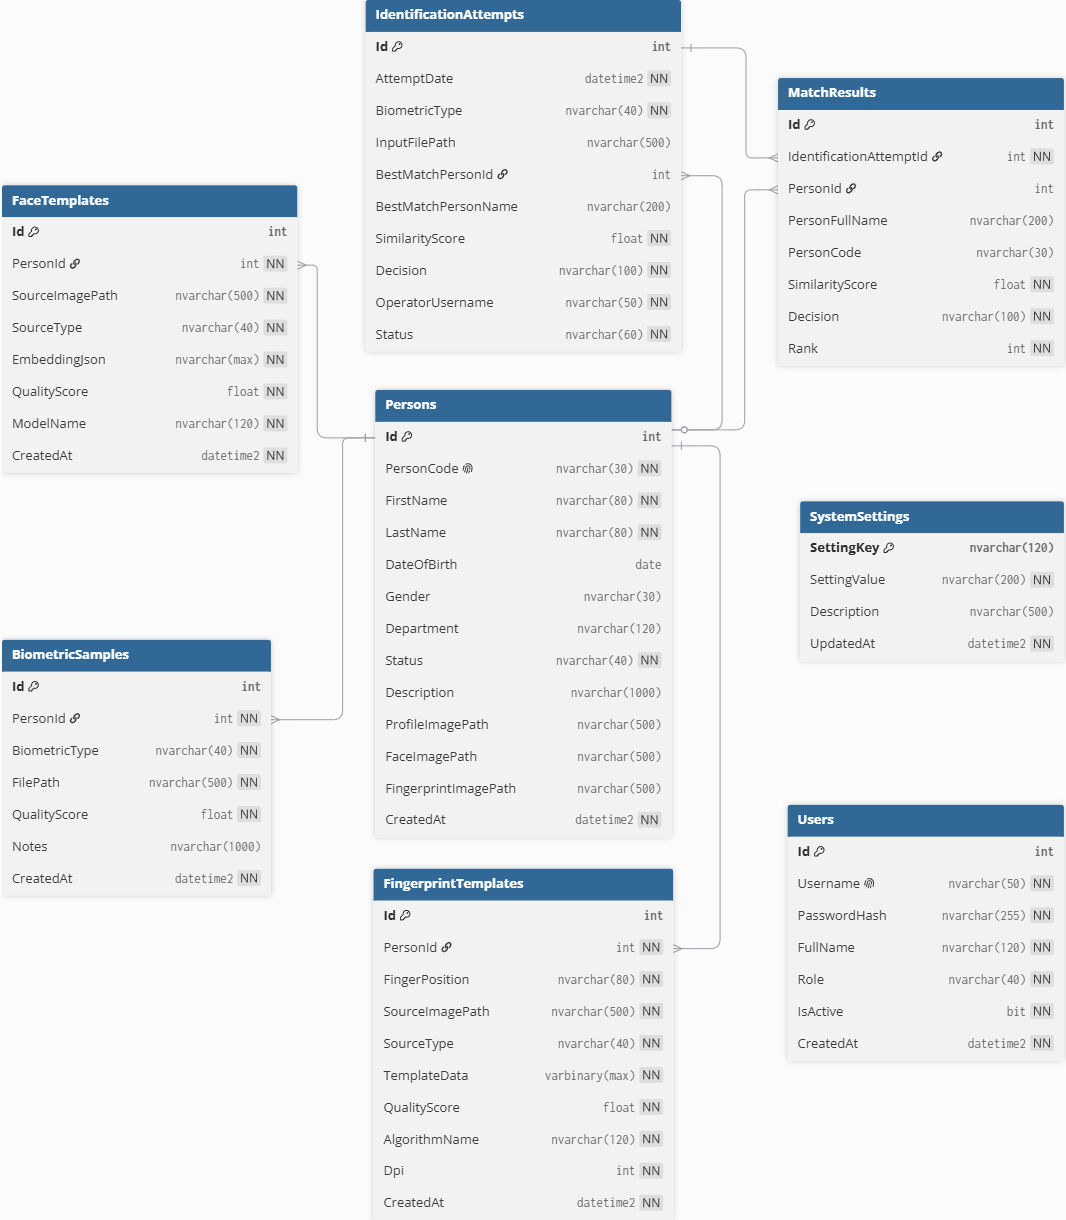
\includegraphics[width=\textwidth]{figures/erd_identitycore.png}
    \caption{Diagram ERD bazy danych systemu IdentityCore}
    \label{fig:erd-identitycore}
\end{figure}

Diagram ułatwia zrozumienie, które tabele stanowią centrum modelu danych oraz w jaki sposób rekordy biometryczne i historia prób są powiązane z osobami zarejestrowanymi w systemie.

\section{Integralność danych}

Integralność danych w bazie wynika przede wszystkim z zastosowania kluczy głównych, kluczy obcych, ograniczeń unikalności oraz wartości domyślnych. Większość głównych tabel posiada klucz główny \texttt{Id} typu całkowitego z automatycznym nadawaniem wartości. Wyjątkiem jest tabela \texttt{SystemSettings}, w której kluczem głównym jest \texttt{SettingKey}.

W tabeli \texttt{Persons} zastosowano unikalny kod osoby zapisany w kolumnie \texttt{PersonCode}. Tabela \texttt{Users} posiada unikalną nazwę użytkownika w kolumnie \texttt{Username}. Ograniczenia te zmniejszają ryzyko duplikowania rekordów o tym samym identyfikatorze logicznym.

Klucze obce wiążą dane biometryczne z osobami oraz wyniki dopasowań z próbami identyfikacji. Tabele \texttt{FaceTemplates}, \texttt{FingerprintTemplates} i \texttt{BiometricSamples} odnoszą się do tabeli \texttt{Persons}, natomiast tabela \texttt{MatchResults} odnosi się do tabeli \texttt{IdentificationAttempts}. Dzięki temu szablony i wyniki nie są przechowywane jako całkowicie oderwane dane.

Oddzielenie danych osób od danych biometrycznych ogranicza duplikację informacji. Dane opisowe osoby nie muszą być powtarzane przy każdym szablonie twarzy lub odcisku palca. W przypadku dodania kolejnych próbek lub szablonów wystarczy utworzyć nowe rekordy powiązane z istniejącą osobą.

\section{Skrypty bazy danych i migracje}

W projekcie zastosowano trzy główne skrypty SQL przechowywane w katalogu \texttt{Database}. Ich zadaniem jest przygotowanie bazy danych, aktualizacja starszej struktury oraz czyszczenie danych biometrycznych podczas testów.

Plik \texttt{create\_database.sql} służy do utworzenia bazy \texttt{IdentityCoreDb} od podstaw. Skrypt tworzy pełną aktualną strukturę tabel, usuwa wcześniej istniejące tabele aplikacji, zakłada klucze, relacje oraz indeksy, a także dodaje podstawowe dane startowe i domyślne ustawienia decyzyjne. Jest to skrypt przeznaczony do świeżej instalacji albo świadomego odtworzenia bazy od zera.

Plik \texttt{update\_existing\_database.sql} służy do aktualizacji starszej istniejącej bazy bez usuwania danych. Skrypt dodaje brakującą kolumnę \texttt{ProfileImagePath}, tworzy tabele \texttt{FaceTemplates}, \texttt{FingerprintTemplates} i \texttt{SystemSettings}, jeżeli ich nie ma, dodaje brakujące indeksy oraz uzupełnia ustawienia systemowe. Zastosowanie instrukcji sprawdzających istnienie tabel, kolumn i indeksów sprawia, że skrypt można traktować jako pomocniczą migrację aktualizującą starszą strukturę.

Plik \texttt{cleanup\_biometric\_data.sql} pełni funkcję testową i porządkową. Umożliwia usunięcie danych dotyczących twarzy i odcisków palców bez usuwania osób z rejestru. Skrypt usuwa powiązane wyniki dopasowań, próby identyfikacji, szablony biometryczne oraz próbki, a także czyści ścieżki do obrazów biometrycznych w tabeli \texttt{Persons}. Na końcu zwraca podstawowe zestawienia kontrolne, które pozwalają sprawdzić stan danych po czyszczeniu.

\section{Uzasadnienie przyjętego modelu danych}

Przyjęty model danych odpowiada potrzebom lokalnej aplikacji desktopowej służącej do identyfikacji osób. Oddzielenie danych opisowych osób od danych biometrycznych ułatwia utrzymanie struktury bazy i pozwala przechowywać wiele szablonów lub próbek dla jednej osoby.

Osobne tabele dla szablonów twarzy, szablonów odcisków palców i próbek biometrycznych pozwalają rozwijać część biometryczną bez zmiany podstawowego rejestru osób. Tabela historii prób oraz tabela wyników kandydatów umożliwiają analizę wykonanych identyfikacji, a tabela ustawień systemowych pozwala przechowywać konfigurację działania aplikacji niezależnie od kodu.
\chapter{Implementacja aplikacji}
\label{chap:implementacja}

\section{Najważniejsze moduły systemu}

Aplikacja \textit{IdentityCore} została zaimplementowana jako lokalna aplikacja desktopowa WPF/.NET. Jej kod podzielono na części odpowiadające głównym funkcjom systemu: logowaniu operatora, rejestrowi osób, identyfikacji twarzy, identyfikacji odcisku palca, historii prób, ustawieniom systemowym oraz komunikacji z bazą danych SQL Server.

Najważniejsze moduły implementacyjne aplikacji przedstawiono w tabeli~\ref{tab:moduly-implementacyjne}. Tabela nie opisuje ponownie architektury całego projektu, lecz pokazuje, które elementy kodu odpowiadają za konkretne funkcje systemu.

\renewcommand{\arraystretch}{1.15}
\begin{xltabular}{\textwidth}{|
    >{\RaggedRight\arraybackslash}p{2.1cm}|
    >{\RaggedRight\arraybackslash}p{7.3cm}|
    >{\RaggedRight\arraybackslash}X|}

    \hline
    \textbf{Moduł} & \textbf{Przykładowe elementy projektu} & \textbf{Rola w aplikacji} \\
    \hline
    \endfirsthead

    \hline
    \textbf{Moduł} & \textbf{Przykładowe elementy projektu} & \textbf{Rola w aplikacji} \\
    \hline
    \endhead

    Logowanie operatora & \texttt{LoginWindow}, \texttt{AuthenticationService}, \texttt{UserRepository} & Sprawdzenie danych operatora i dopuszczenie go do głównej części aplikacji. \\
    \hline
    Rejestr osób & \texttt{PersonRegistryView}, \texttt{PersonRegistryViewModel}, \texttt{PersonRepository} & Dodawanie, odczyt, edycja i usuwanie profili osób zapisanych w systemie. \\
    \hline
    Identyfikacja twarzy & \texttt{FaceIdentificationView}, \texttt{FaceIdentificationViewModel}, \texttt{FaceRecognitionService}, \texttt{FaceEmbeddingService} & Obsługa próby identyfikacji osoby na podstawie obrazu twarzy i reprezentacji uzyskanej z modelu \texttt{arcface.onnx}. \\
    \hline
    Identyfikacja odcisku palca & \texttt{FingerprintIdentificationView}, \texttt{FingerprintIdentificationViewModel}, \texttt{FingerprintRecognitionService} & Obsługa próby identyfikacji osoby na podstawie obrazu odcisku palca i zapisanego szablonu biometrycznego. \\
    \hline
    Obsługa \newline obrazów & \texttt{ImageProcessingService}, \texttt{CameraService} & Przygotowanie danych obrazowych oraz obsługa obrazu pochodzącego z pliku lub kamery. \\
    \hline
    Historia prób & \texttt{HistoryView}, \texttt{HistoryViewModel}, \texttt{IdentificationRepository} & Zapis i odczyt informacji o wykonanych próbach identyfikacji. \\
    \hline
    Ustawienia systemowe & \texttt{SettingsView}, \texttt{SettingsViewModel}, \texttt{SystemSettingsService} & Obsługa parametrów decyzyjnych wykorzystywanych przez moduły biometryczne. \\
    \hline
    Dostęp do danych & \texttt{DatabaseConnection}, \texttt{PersonRepository}, \texttt{FaceTemplateRepository}, \texttt{FingerprintTemplateRepository}, \texttt{BiometricSampleRepository} & Komunikacja z bazą danych SQL Server oraz wykonywanie operacji zapisu, odczytu, aktualizacji i usuwania danych. \\
    \hline
    Modele \newline danych & \texttt{Person}, \texttt{FaceIdentificationResult}, \texttt{FingerprintIdentificationResult}, \texttt{BiometricDecisionSettings}, \texttt{IdentificationAttempt} & Reprezentacja danych przekazywanych między widokami, serwisami i repozytoriami. \\
    \hline
    Nawigacja i komendy & \texttt{MainViewModel}, \texttt{RelayCommand} & Przełączanie głównych widoków aplikacji oraz obsługa akcji wykonywanych przez operatora. \\
    \hline

    \caption{Najważniejsze moduły implementacyjne aplikacji IdentityCore}
    \label{tab:moduly-implementacyjne}
\end{xltabular}

W przedstawionym podziale widoki odpowiadają za prezentację danych, modele widoków za obsługę stanu ekranu i reakcji na działania operatora, serwisy za logikę operacji, a repozytoria za kontakt z bazą danych. Dzięki temu poszczególne funkcje aplikacji są rozdzielone i łatwiejsze do utrzymania.

\section{Implementacja rejestracji osoby}

Rejestracja osoby została zrealizowana w module rejestru osób. Za obsługę tego obszaru odpowiadają przede wszystkim \texttt{PersonRegistryView}, \texttt{PersonRegistryViewModel} oraz \texttt{PersonRepository}. Widok udostępnia formularz danych osoby, model widoku przechowuje aktualnie wybrany profil i obsługuje akcje operatora, a repozytorium wykonuje zapis i odczyt danych z bazy.

Dodanie nowej osoby odbywa się w metodzie \texttt{AddNewPerson}. Tworzony jest nowy obiekt \texttt{Person}, któremu nadawany jest kod osoby, podstawowe dane domyślne, status oraz puste ścieżki do obrazów. Następnie obiekt jest przekazywany do metody \texttt{Add} w klasie \texttt{PersonRepository}. Po zapisie do bazy metoda zwraca identyfikator nowo utworzonego rekordu, który jest przypisywany do obiektu w aplikacji.

Edycja osoby jest realizowana przez metodę \texttt{SaveChanges}. Jeżeli istnieje aktualnie wybrany profil, model widoku przekazuje go do metody \texttt{Update} w \texttt{PersonRepository}. Po aktualizacji dane są ponownie wczytywane, aby lista osób i szczegóły wybranego profilu odpowiadały stanowi zapisanemu w bazie danych.

Podstawowa kontrola poprawności operacji polega między innymi na sprawdzaniu, czy wybrano osobę, na której można wykonać daną akcję. Dotyczy to zapisu zmian, usuwania profilu, ustawiania zdjęcia profilowego oraz rejestrowania danych biometrycznych. Kompletność pól wymaganych jest dodatkowo wymuszana przez model danych i strukturę bazy, której szczegóły opisano w rozdziale~\ref{chap:baza-danych}.

W aplikacji zaimplementowano również obsługę zdjęcia profilowego. Metoda \texttt{SetProfileImage} umożliwia wybór pliku graficznego, skopiowanie go do lokalnego katalogu roboczego aplikacji tworzonego w katalogu uruchomieniowym programu, zapisanie ścieżki w polu \texttt{ProfileImagePath} oraz aktualizację osoby w bazie danych. Usunięcie zdjęcia profilowego realizuje metoda \texttt{RemoveProfileImage}, która czyści ścieżkę i zapisuje zmieniony profil.

\newpage

Dane biometryczne osoby są powiązane z profilem osoby, ale nie są zapisywane jako zwykłe pola formularza opisowego. Rejestracja próbek twarzy i odcisków palców jest obsługiwana przez osobne metody oraz repozytoria biometryczne, między innymi \texttt{FaceTemplateRepository}, \texttt{FingerprintTemplateRepository} i \texttt{BiometricSampleRepository}. Dzięki temu profil osoby pozostaje oddzielony od danych technicznych używanych w procesie identyfikacji.

\section{Implementacja procesu biometrycznego}

Proces biometryczny w aplikacji \textit{IdentityCore} został zaimplementowany jako przepływ danych pomiędzy modelem widoku, usługami biometrycznymi, repozytoriami oraz obiektami wynikowymi. Widok i model widoku odpowiadają za przyjęcie danych od operatora i pokazanie rezultatu, natomiast właściwa analiza biometryczna odbywa się w serwisach. Szczegóły metod identyfikacji zostały opisane w rozdziale~\ref{chap:metody-algorytmy}; w tym miejscu przedstawiono ich praktyczne użycie w kodzie aplikacji.

\subsection{Implementacja identyfikacji twarzy}

Identyfikacja twarzy rozpoczyna się w \texttt{FaceIdentificationViewModel}. Model widoku obsługuje komendy związane z kamerą, wczytaniem obrazu, rozpoczęciem identyfikacji, zapisem próby oraz otwarciem profilu osoby. Obraz wejściowy może pochodzić z pliku wskazanego przez operatora albo z kamery obsługiwanej przez \texttt{CameraService}. W przypadku kamery aplikacja pobiera klatkę, zapisuje ją jako plik wejściowy i dopiero taki obraz przekazuje do dalszej analizy.

Po uruchomieniu identyfikacji \texttt{FaceIdentificationViewModel} wywołuje usługę \texttt{FaceRecognitionService}. Model widoku nie wykonuje samodzielnie porównywania twarzy; jego zadaniem jest przekazanie ścieżki obrazu, obsługa stanu analizy, odebranie wyniku i przepisanie go do właściwości prezentowanych w interfejsie.

Pierwszym ważnym etapem po stronie kodu jest przygotowanie obrazu twarzy. Odpowiada za to \texttt{ImageProcessingService}. Fragment pokazujący przygotowanie próbki twarzy przedstawiono na listingu~\ref{lst:impl-face-prepare-face}.

\lstinputlisting[
    language={[Sharp]C},
    caption={Przygotowanie obrazu twarzy przed analizą},
    label={lst:impl-face-prepare-face}
]{src/face_prepare_face.cs}

W pokazanym fragmencie aplikacja nie przekazuje całego kadru bezpośrednio do modelu. Najpierw wykrywa twarz, przygotowuje wycinek obrazu, sprawdza jego użyteczność, ocenia jakość i skaluje próbkę do wymaganego rozmiaru. Jeżeli nie uda się uzyskać poprawnego obrazu twarzy, dalsza identyfikacja nie jest wykonywana.

Po przygotowaniu próbki wykorzystywany jest \texttt{FaceEmbeddingService}. To w tej usłudze aplikacja używa pliku \texttt{arcface.onnx} i zamienia przygotowany obraz na reprezentację używaną później przy porównywaniu. Fragment tej części implementacji przedstawiono na listingu~\ref{lst:impl-face-embedding-onnx}.

\lstinputlisting[
    language={[Sharp]C},
    caption={Użycie modelu arcface.onnx do wygenerowania embeddingu twarzy},
    label={lst:impl-face-embedding-onnx}
]{src/face_embedding_onnx.cs}

Listing pokazuje miejsce, w którym aplikacja odnajduje model \texttt{arcface.onnx}, tworzy potok ONNX i uruchamia predykcję dla przygotowanego obrazu twarzy. Wynikiem działania tej usługi jest reprezentacja przekazywana dalej do \texttt{FaceRecognitionService}.

Kolejnym etapem jest pobranie zapisanych wzorców twarzy i utworzenie rankingu kandydatów. Wykorzystywane są tutaj \texttt{FaceTemplateRepository} oraz \texttt{PersonRepository}. Fragment odpowiedzialny za ten etap przedstawiono na listingu~\ref{lst:impl-face-candidate-selection}.

\lstinputlisting[
    language={[Sharp]C},
    caption={Wybór kandydatów podczas identyfikacji twarzy},
    label={lst:impl-face-candidate-selection}
]{src/face_candidate_selection.cs}

W tym fragmencie aplikacja pobiera zapisane szablony twarzy, łączy je z osobami z rejestru, odczytuje zapisane reprezentacje i porównuje je z próbką wejściową. Wyniki są grupowane według osoby, ponieważ jedna osoba może posiadać więcej niż jeden zapisany szablon. Następnie tworzony jest ranking najlepszych kandydatów.

Samo porównanie dwóch reprezentacji twarzy zostało wydzielone do osobnego fragmentu. Listing~\ref{lst:impl-cosine-similarity} pokazuje implementację obliczenia wyniku podobieństwa wykorzystywanego podczas budowania rankingu kandydatów.

\lstinputlisting[
    language={[Sharp]C},
    caption={Obliczanie podobieństwa cosinusowego dla embeddingów twarzy},
    label={lst:impl-cosine-similarity}
]{src/cosine_similarity.cs}

W pokazanym fragmencie kod sprawdza poprawność porównywanych wektorów, oblicza wynik podobieństwa i ogranicza go do zakresu procentowego. Wartość zwrócona przez tę metodę jest później używana przy wyborze najlepszego kandydata i ocenie, czy wynik spełnia wymagania decyzyjne.

Po utworzeniu listy kandydatów \texttt{FaceRecognitionService} wybiera najlepszy wynik i porównuje go z drugim kandydatem. W tym miejscu stosowane są ustawienia decyzyjne pobrane z \texttt{SystemSettingsService}, czyli próg dopasowania oraz minimalny margines. Jeżeli w bazie nie ma wzorców twarzy, nie uda się odczytać poprawnych danych, na obrazie nie wykryto twarzy albo wynik jest zbyt słaby, aplikacja zwraca decyzję o braku dopasowania wraz z komunikatem opisującym problem.

\subsection{Implementacja identyfikacji odcisku palca}

Identyfikacja odcisku palca rozpoczyna się w \texttt{FingerprintIdentificationViewModel}. Model widoku obsługuje wczytanie obrazu odcisku z pliku, rozpoczęcie analizy, zapis próby oraz otwarcie profilu osoby. Po wybraniu pliku ścieżka obrazu jest zapisywana jako \texttt{InputFilePath}, a następnie przekazywana do \texttt{FingerprintRecognitionService}.

Właściwa logika biometryczna znajduje się w \texttt{FingerprintRecognitionService}. Pierwszym kluczowym etapem jest utworzenie szablonu próbki wejściowej. Fragment odpowiedzialny za zamianę obrazu odcisku na dane szablonu przedstawiono na listingu~\ref{lst:impl-fingerprint-template-creation}.

\lstinputlisting[
    language={[Sharp]C},
    caption={Utworzenie szablonu odcisku palca na podstawie obrazu wejściowego},
    label={lst:impl-fingerprint-template-creation}
]{src/fingerprint_template_creation.cs}

W pokazanym fragmencie aplikacja sprawdza, czy plik obrazu istnieje, odczytuje jego zawartość i tworzy szablon próbki wejściowej. Jeżeli plik nie zostanie znaleziony, nie można go odczytać albo szablon jest pusty, metoda zwraca wynik niepowodzenia z komunikatem.

\newpage

Po utworzeniu szablonu próbki aplikacja pobiera zapisane szablony odcisków palców przez \texttt{FingerprintTemplateRepository} oraz dane osób przez \texttt{PersonRepository}. Następnie próbka wejściowa jest porównywana z kolejnymi wzorcami zapisanymi w bazie. Fragment tej części procesu przedstawiono na listingu~\ref{lst:impl-fingerprint-matching-flow}.

\lstinputlisting[
    language={[Sharp]C},
    caption={Porównywanie próbki odcisku palca z zapisanymi szablonami},
    label={lst:impl-fingerprint-matching-flow}
]{src/fingerprint_matching_flow.cs}

Listing pokazuje, jak aplikacja tworzy matcher dla próbki wejściowej, przechodzi po zapisanych szablonach, pomija rekordy bez osoby albo bez danych szablonu i wylicza wynik dopasowania. Dla każdego poprawnego porównania tworzony jest obiekt kandydata zawierający dane osoby oraz wynik podobieństwa.

Po zebraniu wyników aplikacja wybiera najlepszych kandydatów i ocenia, czy wynik może zostać zaakceptowany. Fragment logiki decyzyjnej przedstawiono na listingu~\ref{lst:impl-fingerprint-decision-threshold}.

\lstinputlisting[
    language={[Sharp]C},
    caption={Decyzja identyfikacyjna na podstawie progu i marginesu dopasowania},
    label={lst:impl-fingerprint-decision-threshold}
]{src/fingerprint_decision_threshold.cs}

W tym fragmencie najlepszy wynik jest porównywany z wymaganym progiem dopasowania, a następnie sprawdzana jest różnica względem drugiego kandydata. Jeżeli wynik jest zbyt niski albo przewaga nad kolejnym kandydatem jest niewystarczająca, próba nie zostaje uznana za dopasowanie. Do modelu widoku trafia wtedy wynik negatywny wraz z informacją diagnostyczną.

Wynik działania \texttt{FingerprintRecognitionService} jest przekazywany z powrotem do \texttt{FingerprintIdentificationViewModel}. Model widoku aktualizuje dane najlepszego kandydata, wynik, decyzję, komunikat, próg, margines oraz listę kandydatów. Dzięki temu warstwa interfejsu otrzymuje gotowy rezultat próby bez wykonywania logiki porównywania w samym widoku.

\subsection{Zapis wyniku identyfikacji w historii}

Po zakończeniu próby identyfikacji aplikacja przygotowuje obiekt \texttt{IdentificationAttempt}. Jest on tworzony po stronie modelu widoku na podstawie wyniku zwróconego przez serwis biometryczny. Do obiektu trafiają dane opisujące próbę, między innymi typ biometrii, ścieżka pliku wejściowego, najlepiej dopasowana osoba, wynik podobieństwa, decyzja, operator, status oraz data wykonania próby.

Sam zapis do bazy danych wykonuje \texttt{IdentificationRepository}. Fragment metody zapisującej próbę identyfikacji przedstawiono na listingu~\ref{lst:impl-identification-add-attempt}.

\lstinputlisting[
    language={[Sharp]C},
    caption={Zapis próby identyfikacji do historii},
    label={lst:impl-identification-add-attempt}
]{src/identification_add_attempt.cs}

W pokazanym fragmencie repozytorium tworzy polecenie SQL i przekazuje do niego wartości z obiektu \texttt{IdentificationAttempt}. Po wykonaniu zapytania zwracany jest identyfikator nowo zapisanego rekordu. Mechanizm ten pozwala później odtworzyć wykonane próby i wykorzystać je podczas analizy skuteczności opisanej w rozdziale testowym.

\section{Implementacja logowania i autoryzacji}

Logowanie operatora zostało zrealizowane jako prosta część techniczna aplikacji. Użytkownik najpierw trafia do okna \texttt{LoginWindow}, gdzie podaje dane logowania. Dopiero po poprawnym uwierzytelnieniu otwierana jest główna część systemu.

Za sprawdzenie danych odpowiada \texttt{AuthenticationService}. Usługa korzysta z \texttt{UserRepository}, które wyszukuje aktywnego użytkownika w bazie danych na podstawie nazwy użytkownika. Jeżeli użytkownik nie istnieje, jest nieaktywny albo hasło nie pasuje do wartości zapisanej w bazie, logowanie kończy się niepowodzeniem.

Fragment logiki sprawdzania danych logowania przedstawiono na listingu~\ref{lst:impl-authentication-login}.

\lstinputlisting[
    language={[Sharp]C},
    caption={Sprawdzenie danych logowania operatora},
    label={lst:impl-authentication-login}
]{src/authentication_login.cs}

W pokazanym fragmencie metoda odrzuca puste dane, pobiera aktywnego użytkownika z bazy i porównuje podane hasło z wartością zapisaną w rekordzie użytkownika. Po poprawnym sprawdzeniu ustawiany jest aktualny użytkownik aplikacji.

W aktualnej postaci logowanie ma charakter demonstracyjny i techniczny. W kodzie hasło jest porównywane z wartością przechowywaną w polu \texttt{PasswordHash}, ale nie zaimplementowano rozbudowanego mechanizmu bezpieczeństwa typowego dla systemów produkcyjnych. Jest to wystarczające dla lokalnej aplikacji projektowej, której celem jest prezentacja działania systemu identyfikacji biometrycznej.

Dane konta testowego oraz instrukcja uruchomienia aplikacji nie są rozwijane w tym miejscu, ponieważ zostaną opisane w rozdziale dotyczącym uruchomienia projektu.

\section{Operacje CRUD}

Operacje CRUD są wykonywane głównie w module rejestru osób. Klasa \texttt{PersonRepository} zawiera metody \texttt{GetAll}, \texttt{Add}, \texttt{Update}, \texttt{GetById} oraz \texttt{Delete}. Dzięki temu aplikacja może odczytywać listę osób, dodawać nowe profile, aktualizować dane, pobierać pojedynczą osobę oraz usuwać rekord osoby z bazy.

Odczyt listy osób odbywa się w metodzie \texttt{LoadPersons} w \texttt{PersonRegistryViewModel}. Metoda czyści aktualną kolekcję \texttt{Persons}, pobiera dane przez \texttt{PersonRepository.GetAll}, a następnie uzupełnia kolekcję używaną przez widok. Po wczytaniu danych aktualizowane są również liczniki osób i danych biometrycznych.

Dodanie osoby jest realizowane przez \texttt{AddNewPerson}, natomiast zapis zmian przez \texttt{SaveChanges}. Usuwanie profilu obsługuje metoda \texttt{DeleteSelectedPerson}, która wywołuje \texttt{PersonRepository.Delete}, usuwa obiekt z kolekcji oraz aktualizuje wybór aktualnej osoby.

Operacje związane z ustawieniami systemowymi są realizowane przez \texttt{SettingsViewModel} oraz \texttt{SystemSettingsService}. Pozwalają one odczytywać i zapisywać wartości parametrów decyzyjnych bez modyfikowania kodu aplikacji.

Historia prób identyfikacji jest obsługiwana przez \texttt{IdentificationRepository}. Repozytorium zawiera metody służące do pobierania prób oraz zapisywania nowej próby identyfikacji. Dzięki temu wyniki pracy modułów biometrycznych nie znikają po zakończeniu operacji, lecz są utrwalane w bazie danych.

W tym rozdziale nie przedstawiono pełnych zapytań SQL dla każdej operacji, ponieważ struktura bazy i skrypty zostały omówione w rozdziale~\ref{chap:baza-danych}. W kontekście implementacji istotne jest to, że operacje na danych są wykonywane przez repozytoria, a nie bezpośrednio w widokach WPF.

\section{Nawigacja i przepływ danych w aplikacji}

Nawigacja w aplikacji jest obsługiwana przez \texttt{MainViewModel}. Klasa ta przechowuje aktualnie wybrany model widoku w polu \texttt{CurrentViewModel}. Na tej podstawie główne okno aplikacji wyświetla odpowiedni obszar systemu.

Przełączanie widoków odbywa się przez komendy, między innymi \texttt{ShowDashboardCommand}, \texttt{ShowPersonRegistryCommand}, \texttt{ShowFaceIdentificationCommand}, \newline \texttt{ShowFingerprintIdentificationCommand}, \texttt{ShowHistoryCommand} oraz \newline \texttt{ShowSettingsCommand}. Każda z nich ustawia właściwy model widoku, aktywny klucz strony, tytuł oraz podtytuł aktualnego ekranu.

W aplikacji wykorzystywana jest klasa \texttt{RelayCommand}, która pozwala powiązać akcje interfejsu z metodami modeli widoków. Dzięki temu logika działania nie musi być umieszczana bezpośrednio w plikach XAML. Widok wywołuje komendę, a model widoku wykonuje odpowiednią operację.

Przepływ danych polega na tym, że widok prezentuje dane z modelu widoku, a model widoku korzysta z serwisów i repozytoriów. Po wykonaniu operacji dane są odświeżane, na przykład przez ponowne wczytanie listy osób albo aktualizację wyników identyfikacji. Komunikaty zwrotne są przekazywane przez właściwości takie jak \texttt{ErrorMessage} i \texttt{StatusMessage}.

Z poziomu \texttt{MainViewModel} możliwe jest również otwarcie profilu konkretnej osoby w rejestrze. Metoda \texttt{OpenPersonProfile} przełącza aplikację do rejestru osób i wskazuje wybrany profil na podstawie identyfikatora.
\chapter{Prezentacja warstwy użytkowej}
\label{chap:warstwa-uzytkowa}

\section{Ogólny układ interfejsu}

Warstwa użytkowa aplikacji \textit{IdentityCore} została przygotowana jako lokalny interfejs desktopowy utrzymany w ciemnym motywie. Po zalogowaniu większość widoków korzysta z tego samego układu: po lewej stronie znajduje się pionowe menu nawigacyjne z nazwą aplikacji, a po prawej główny obszar roboczy danego modułu. Aktualnie wybrany moduł jest wyróżniony innym tłem oraz akcentem kolorystycznym, dzięki czemu operator od razu widzi, w której części systemu aktualnie pracuje.

Wspólne menu boczne umożliwia przejście do panelu głównego, rejestru osób, identyfikacji twarzy, identyfikacji odcisku palca, historii prób oraz ustawień. W górnej części obszaru roboczego znajduje się tytuł widoku, krótki opis funkcji modułu oraz przycisk \texttt{Wyloguj}. Taki układ porządkuje sposób korzystania z aplikacji: operator najpierw wybiera moduł z menu, następnie pracuje w jego głównym panelu, a wyniki lub komunikaty są prezentowane w wydzielonych sekcjach widoku.

\section{Ekran logowania}

Pierwszym ekranem aplikacji jest ekran logowania. Jego zadaniem jest ograniczenie dostępu do głównej części systemu tylko do operatora posiadającego dane dostępowe. Po lewej stronie ekranu pokazano nazwę aplikacji, jej ogólne przeznaczenie oraz zakres dostępnych modułów. Po prawej stronie znajduje się formularz logowania z polami \texttt{Login} i \texttt{Hasło} oraz przyciskiem \texttt{Zaloguj}. Widoczna jest również informacja o koncie testowym, która ułatwia uruchomienie aplikacji w środowisku demonstracyjnym.
\begin{figure}[H]
    \centering
    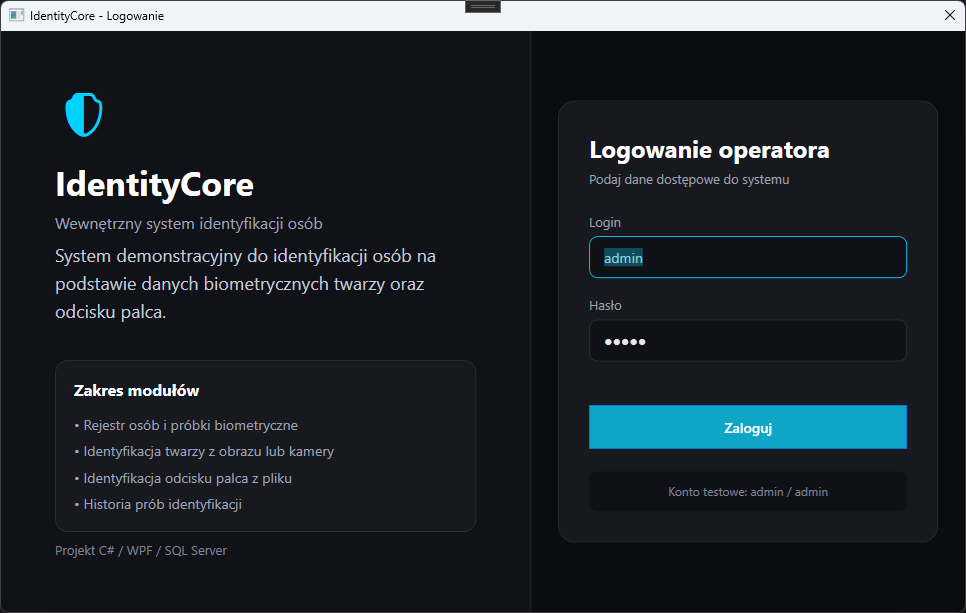
\includegraphics[width=0.98\textwidth]{figures/ui/ui_01_login.png}
    \caption{Ekran logowania do aplikacji IdentityCore}
    \label{fig:ui-login}
\end{figure}

\newpage

\section{Panel główny aplikacji}

Po poprawnym zalogowaniu operator trafia do panelu głównego. Jest to ekran podsumowujący aktualny stan systemu oraz najważniejsze dane zapisane w aplikacji. W górnej części panelu znajdują się kafle informujące o liczbie osób w bazie, liczbie osób z danymi biometrycznymi, liczbie szablonów twarzy, liczbie szablonów odcisków oraz liczbie zapisanych prób identyfikacji. Dzięki temu operator od razu widzi, czy system posiada dane potrzebne do wykonywania identyfikacji.

\bigskip

Centralna część panelu głównego prezentuje ostatnie próby identyfikacji. W tabeli widoczna jest data i czas próby, typ biometrii, dopasowanie, wynik oraz decyzja systemu. Prawa część widoku pokazuje gotowość danych biometrycznych, aktualne parametry rozpoznawania oraz szybkie przejścia do najważniejszych funkcji. Z tego miejsca operator może szybko przejść do rejestru osób, identyfikacji twarzy, identyfikacji odcisku lub historii prób, bez konieczności ręcznego wyszukiwania odpowiedniej funkcji w systemie.

\bigskip

\begin{figure}[H]
    \centering
    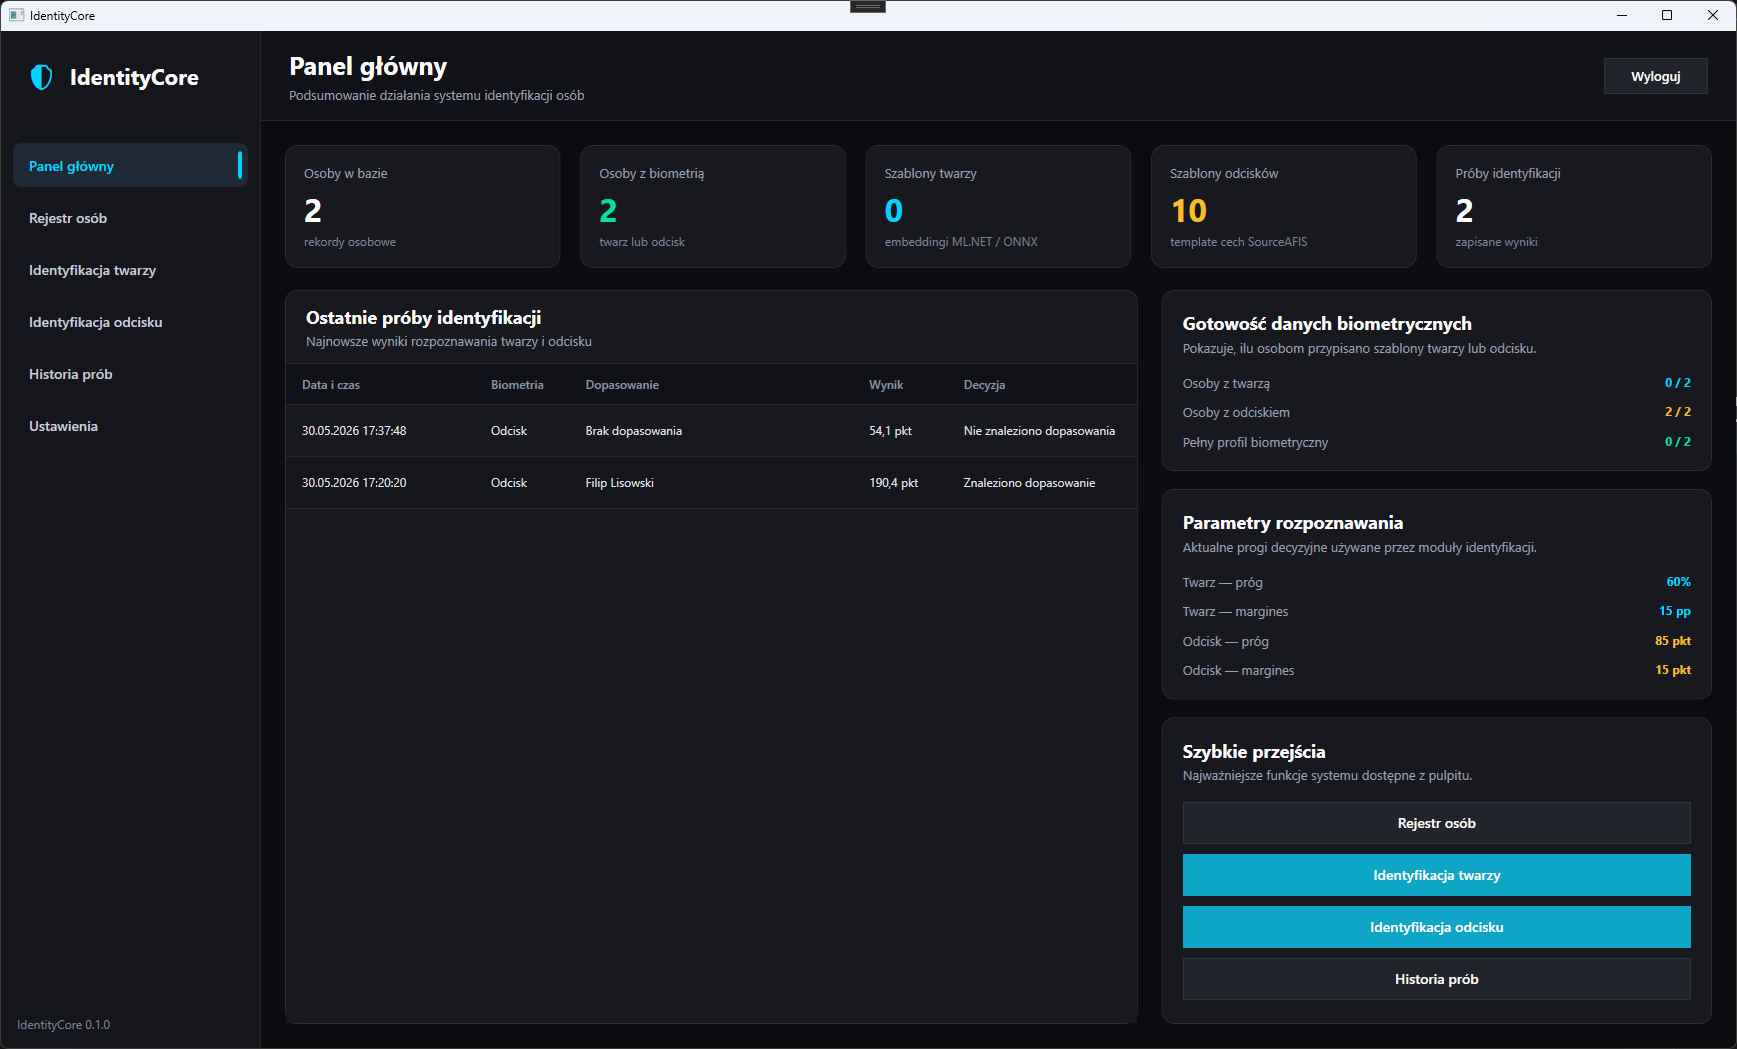
\includegraphics[width=0.98\textwidth]{figures/ui/ui_02_dashboard.png}
    \caption{Panel główny aplikacji po zalogowaniu}
    \label{fig:ui-dashboard}
\end{figure}

\newpage

\section{Rejestr osób i profil osoby}

Widok rejestru osób łączy listę osób zapisanych w systemie z panelem szczegółów aktualnie wybranego profilu. W górnej części widoku znajdują się kafle podsumowujące liczbę osób w bazie, liczbę osób z przypisanymi danymi biometrycznymi oraz liczbę próbek twarzy i odcisków. Poniżej, po lewej stronie, znajduje się tabela osób zawierająca identyfikator osoby, imię i nazwisko, dział lub jednostkę oraz datę dodania. Z poziomu tabeli operator może otworzyć wybrany profil.

\bigskip

Prawa część widoku przedstawia panel profilu osoby. Zawiera zdjęcie profilowe, podstawowe dane osoby, informacje o próbkach twarzy i odcisku palca oraz przyciski umożliwiające rejestrację danych biometrycznych. W tym samym obszarze znajdują się pola edycji danych osobowych oraz przyciski \texttt{Zapisz zmiany} i \texttt{Usuń osobę}. Dzięki temu widok rejestru pełni jednocześnie funkcję listy osób, panelu szczegółów oraz miejsca zarządzania podstawowymi danymi osoby i jej materiałem biometrycznym.

\bigskip

\begin{figure}[H]
    \centering
    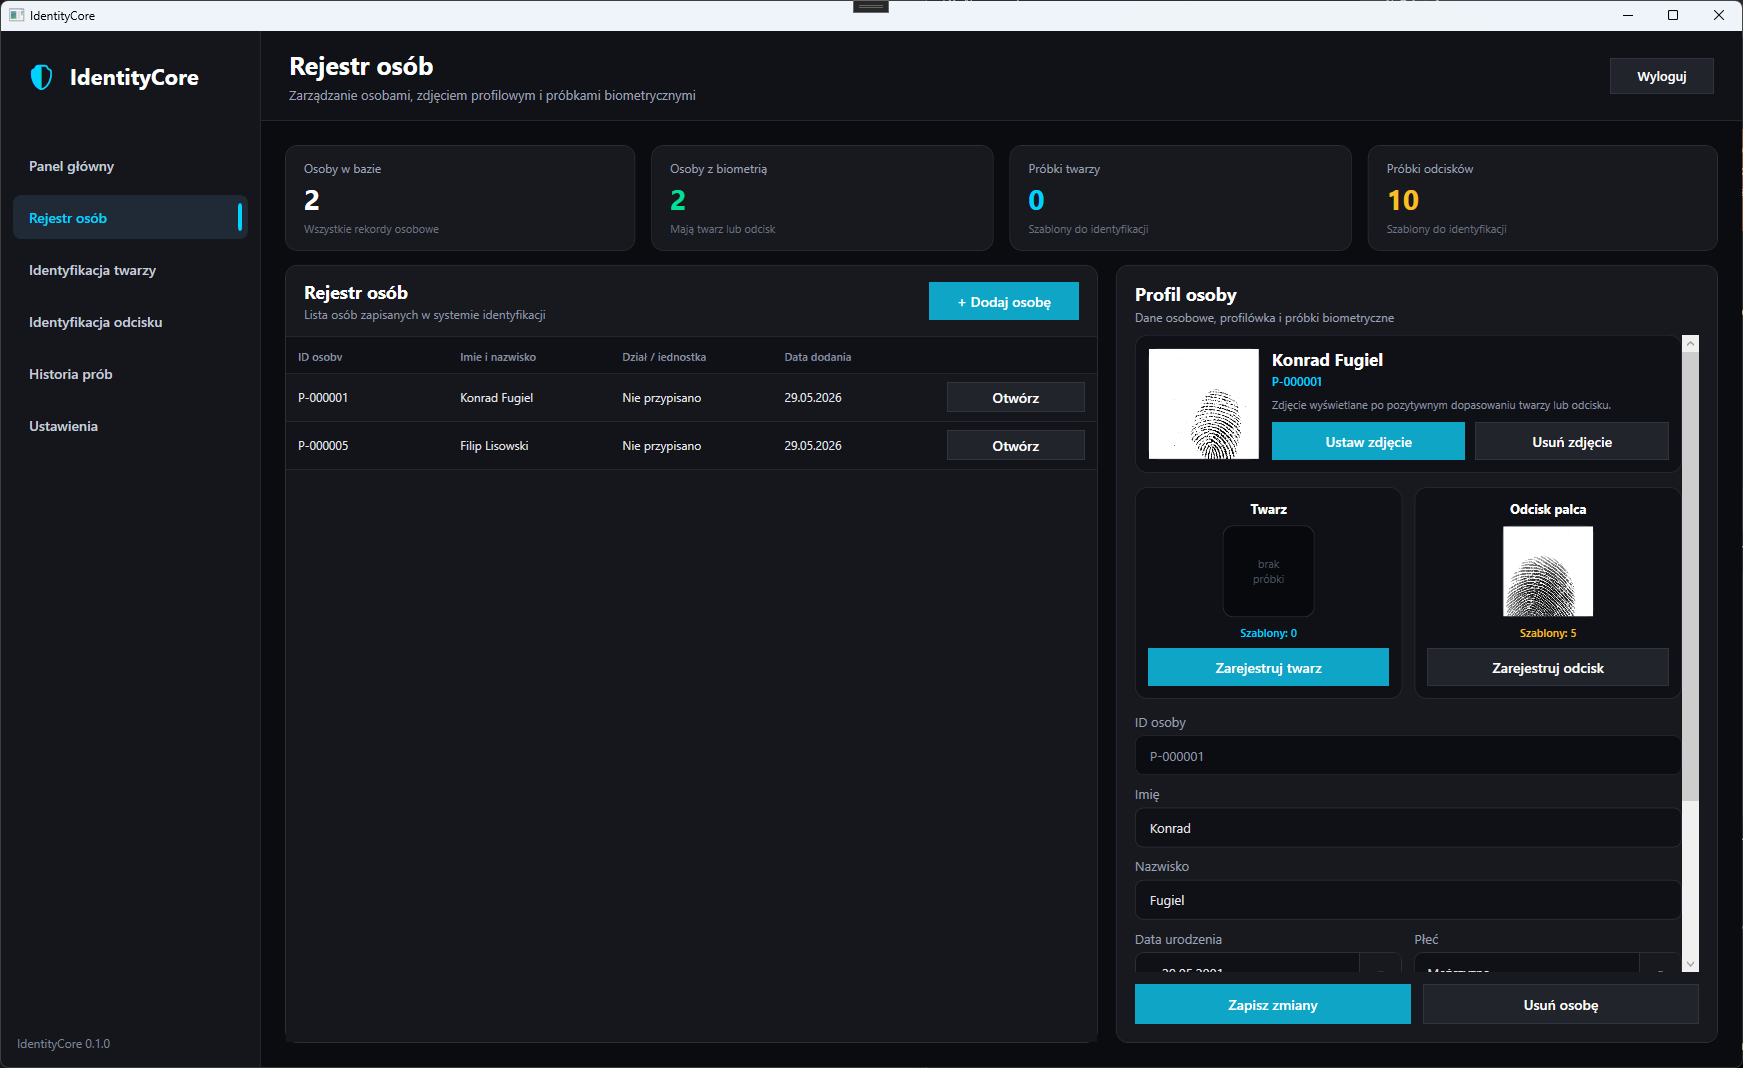
\includegraphics[width=0.98\textwidth]{figures/ui/ui_03_person_registry.png}
    \caption{Rejestr osób wraz z panelem profilu wybranej osoby}
    \label{fig:ui-person-registry}
\end{figure}

\newpage

\section{Widok identyfikacji twarzy}

Widok identyfikacji twarzy został podzielony na trzy główne obszary: źródło biometryczne, analizę biometryczną oraz wynik identyfikacji. Po lewej stronie znajduje się panel z podglądem obrazu oraz przyciskami \texttt{Uruchom kamerę}, \texttt{Wyłącz kamerę}, \texttt{Zrób zdjęcie} i \texttt{Wczytaj obraz}. Oznacza to, że operator może skorzystać zarówno z kamery, jak i z wcześniej przygotowanego pliku graficznego. Widok jasno informuje, że obsługiwane źródła to kamera internetowa oraz pliki obrazów.

\bigskip

Środkowa część widoku prezentuje przebieg analizy. Pokazane są informacje o modelu, jakości próbki, źródle danych oraz bazie wzorców. Poniżej znajduje się lista etapów, takich jak detekcja twarzy, normalizacja obrazu, ekstrakcja cech, porównanie z bazą oraz decyzja systemu. Na dole widoczny jest pasek postępu i przycisk uruchamiający identyfikację. Prawy panel służy do prezentacji wyniku: pokazuje najlepsze dopasowanie, dane osoby, wynik podobieństwa, decyzję systemu oraz listę najbliższych dopasowań. W stanie początkowym aplikacja informuje, że analiza nie została jeszcze wykonana.

\bigskip

\begin{figure}[H]
    \centering
    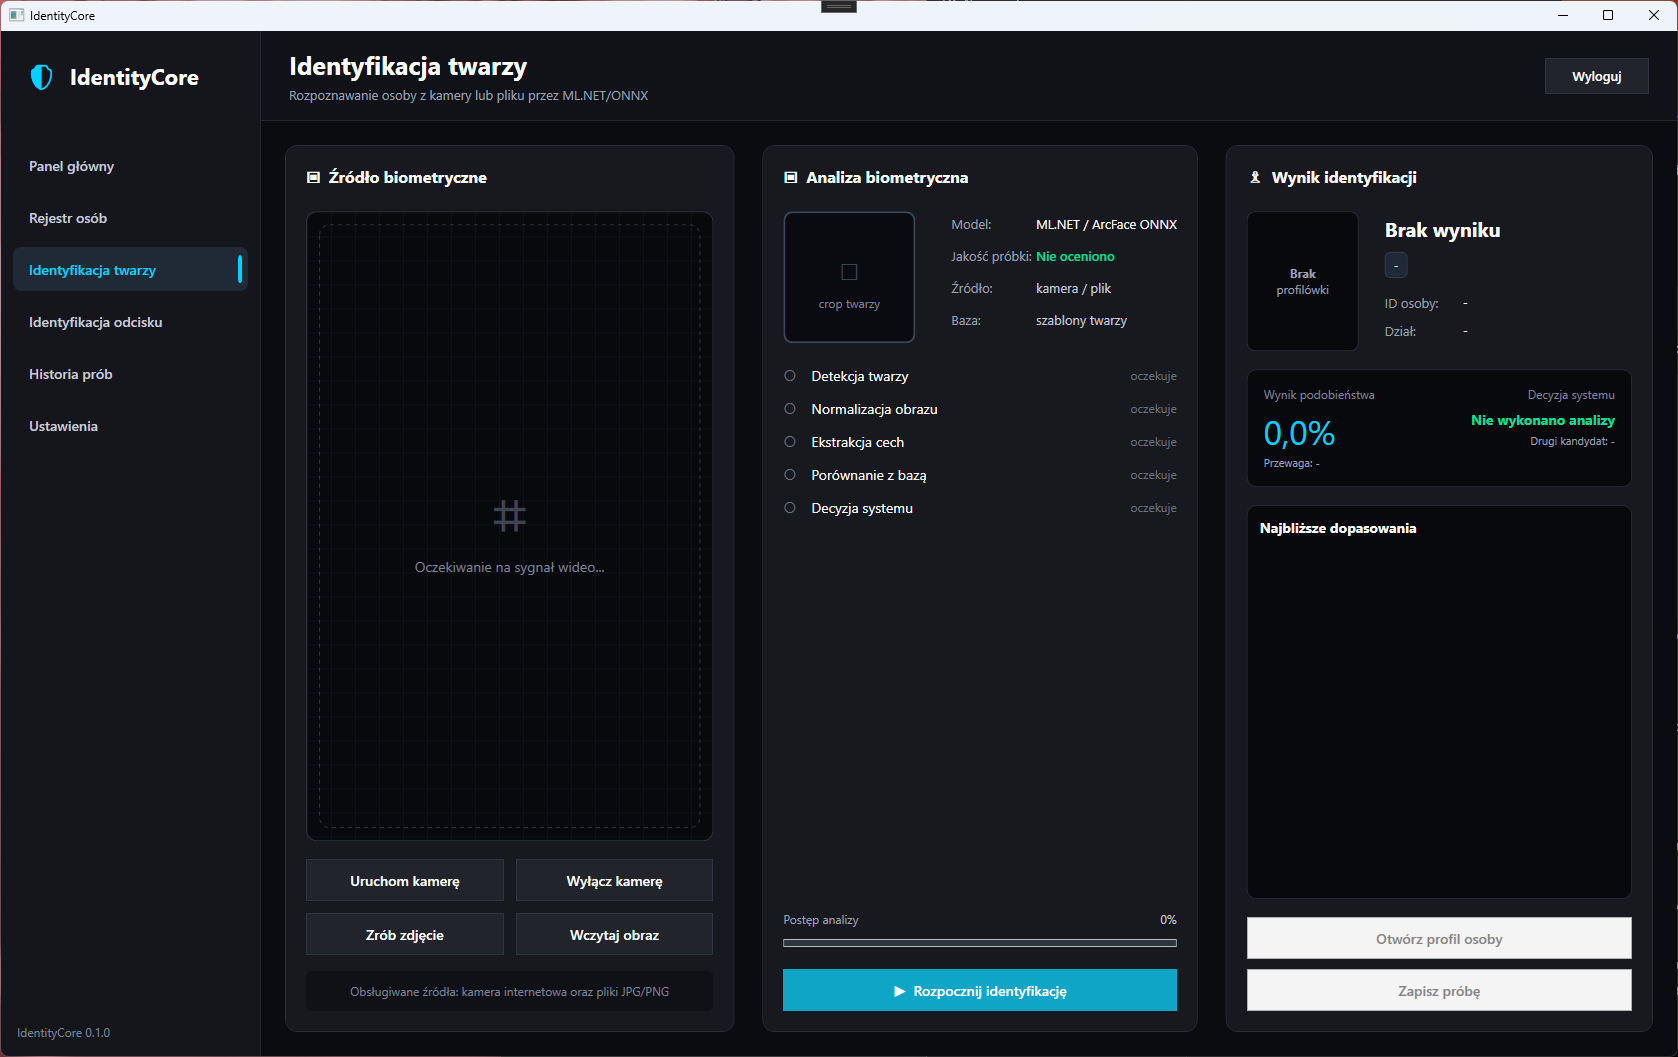
\includegraphics[width=0.98\textwidth]{figures/ui/ui_04_face_identification_input.png}
    \caption{Widok identyfikacji twarzy przed uruchomieniem analizy}
    \label{fig:ui-face-identification}
\end{figure}

\newpage

\section{Widok identyfikacji odcisku palca}

Widok identyfikacji odcisku palca ma podobny układ do modułu twarzy, ale jest dostosowany do pracy z obrazem odcisku. Lewy panel odpowiada za źródło biometryczne i umożliwia wczytanie obrazu odcisku palca z pliku. Widoczny jest duży obszar przeznaczony na podgląd próbki oraz przycisk \texttt{Wczytaj obraz odcisku}. Pod panelem znajduje się informacja o obsługiwanych formatach obrazów oraz o tym, że próbki mogą pochodzić z aplikacji skanera.

\bigskip

Środkowa część widoku pokazuje analizę odcisku palca. Operator widzi informacje o szablonie, cechach, progu oraz kontroli, a także kolejne etapy analizy: wczytanie obrazu, utworzenie template cech, porównanie template z bazą, ocenę wyniku dopasowania i decyzję systemu. Na dole znajduje się pasek postępu oraz przycisk rozpoczęcia analizy. Prawy panel prezentuje najlepsze dopasowanie, identyfikator osoby, dział, wynik punktowy oraz decyzję. W stanie początkowym widok pokazuje brak wyniku i informację, że analiza nie została jeszcze wykonana.

\bigskip

\begin{figure}[H]
    \centering
    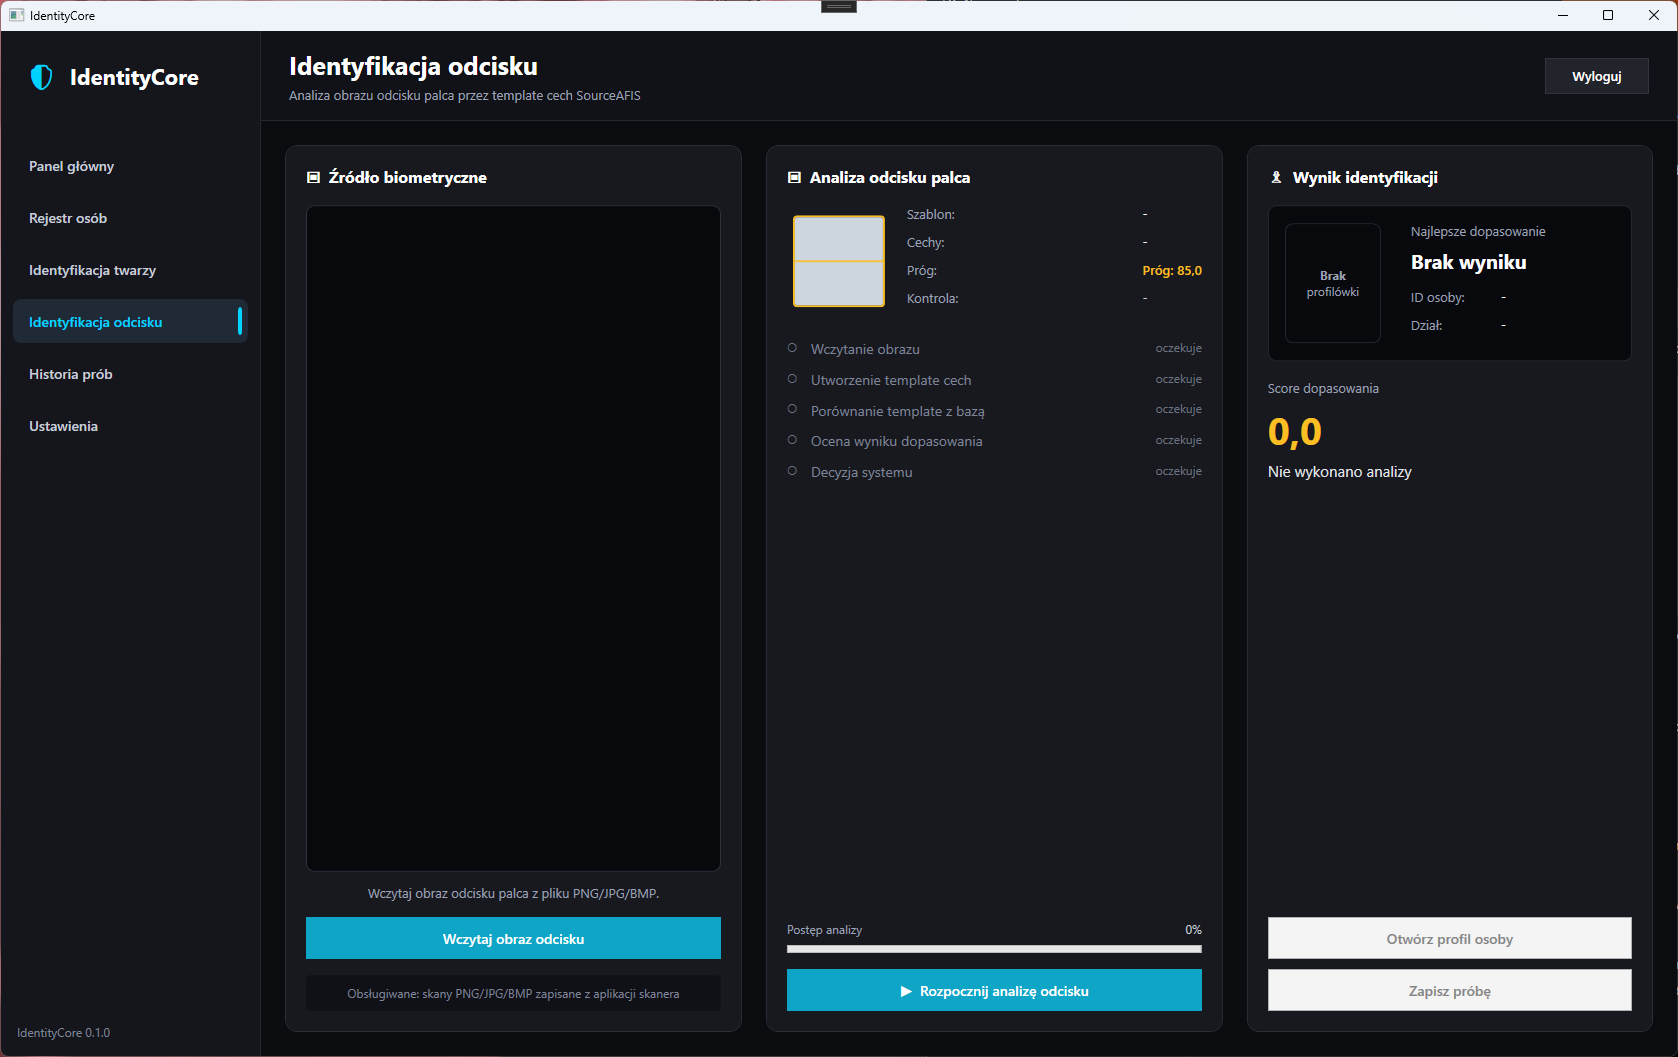
\includegraphics[width=0.98\textwidth]{figures/ui/ui_05_fingerprint_identification_input.png}
    \caption{Widok identyfikacji odcisku palca przed uruchomieniem analizy}
    \label{fig:ui-fingerprint-identification}
\end{figure}

\newpage

\section{Historia prób identyfikacji}

Widok historii prób identyfikacji służy do przeglądania zapisanych zdarzeń związanych z analizą twarzy i odcisku palca. W górnej części ekranu znajdują się liczniki przedstawiające łączną liczbę prób, liczbę znalezionych dopasowań oraz liczbę prób bez dopasowania. Niżej umieszczono tabelę historii, w której widoczne są takie informacje jak data i czas próby, typ biometrii, dopasowanie, wynik, decyzja oraz plik wejściowy. Nad tabelą znajdują się filtry oraz przycisk odświeżania danych.

\bigskip

Po prawej stronie widoku znajduje się panel szczegółów wybranej próby. Pokazuje on wynik, datę próby, typ biometrii, najlepsze dopasowanie oraz plik wejściowy. Taki układ pozwala operatorowi najpierw przeglądać zbiorczą listę prób, a następnie odczytać szczegóły konkretnego zdarzenia bez przechodzenia do innego modułu. Widok historii nie służy w tym rozdziale do oceny skuteczności systemu, ale pokazuje, w jaki sposób aplikacja prezentuje zapisane wyniki pracy modułów identyfikacji.

\bigskip

\begin{figure}[H]
    \centering
    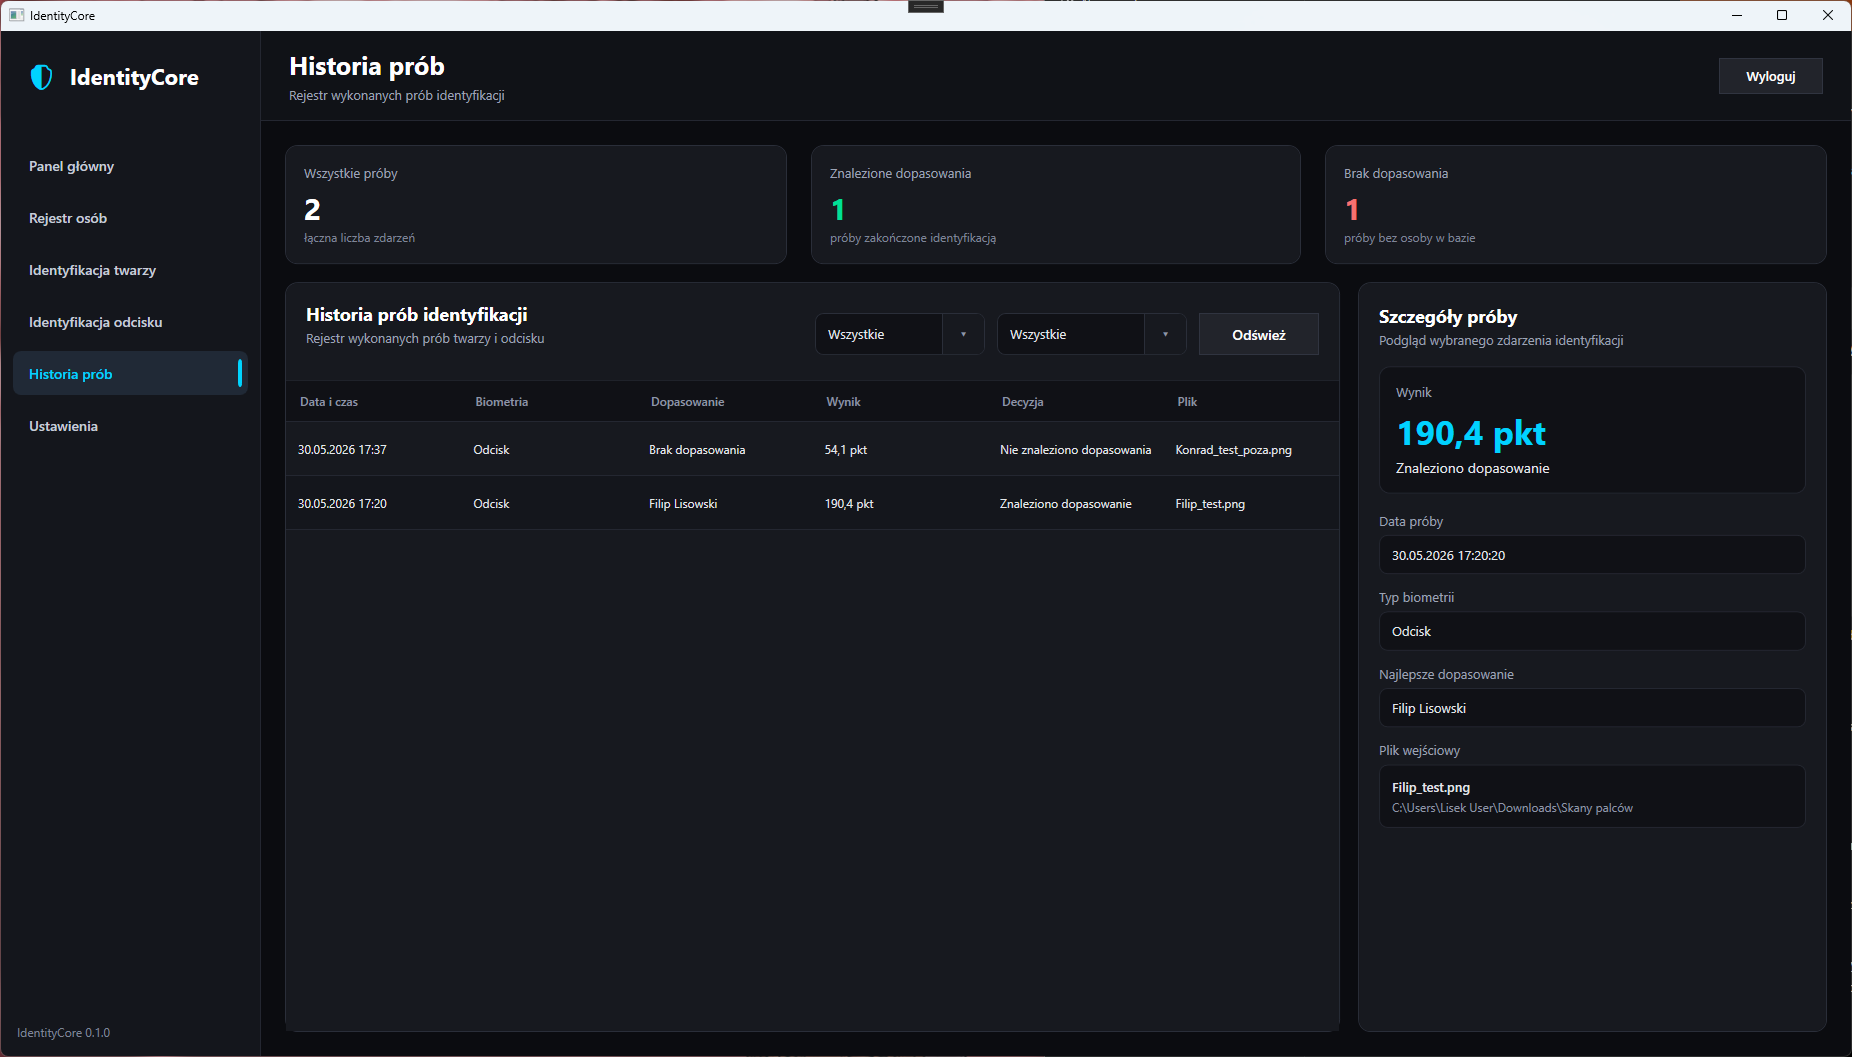
\includegraphics[width=0.98\textwidth]{figures/ui/ui_09_history.png}
    \caption{Widok historii prób identyfikacji}
    \label{fig:ui-history}
\end{figure}

\newpage

\section{Ustawienia systemu}

Widok ustawień prezentuje parametry decyzyjne oraz informacje o modułach biometrycznych. W górnej części ekranu znajdują się kafle opisujące moduł twarzy, moduł odcisku palca oraz sposób prezentacji decyzji systemu. W głównej części widoku umieszczono suwaki i pola wartości dla progów oraz marginesów: minimalnego wyniku podobieństwa twarzy, minimalnej przewagi nad drugim kandydatem, minimalnego wyniku SourceAFIS oraz minimalnej przewagi dla odcisku palca.

\bigskip

Prawa część widoku zawiera informacje o ustawieniach systemu, wykorzystywanych modułach oraz zasobach lokalnych. Widoczne są między innymi odniesienia do modelu \texttt{MLModels/arcface.onnx} oraz katalogów używanych przez aplikację. Na dole panelu znajdują się przyciski \texttt{Zapisz progi} i \texttt{Domyślne}. Pierwszy służy do zapisania aktualnie ustawionych wartości, a drugi do przywrócenia parametrów domyślnych. W tym rozdziale ustawienia są opisane wyłącznie jako element interfejsu, bez analizowania ich wpływu na wyniki identyfikacji.

\bigskip

\begin{figure}[H]
    \centering
    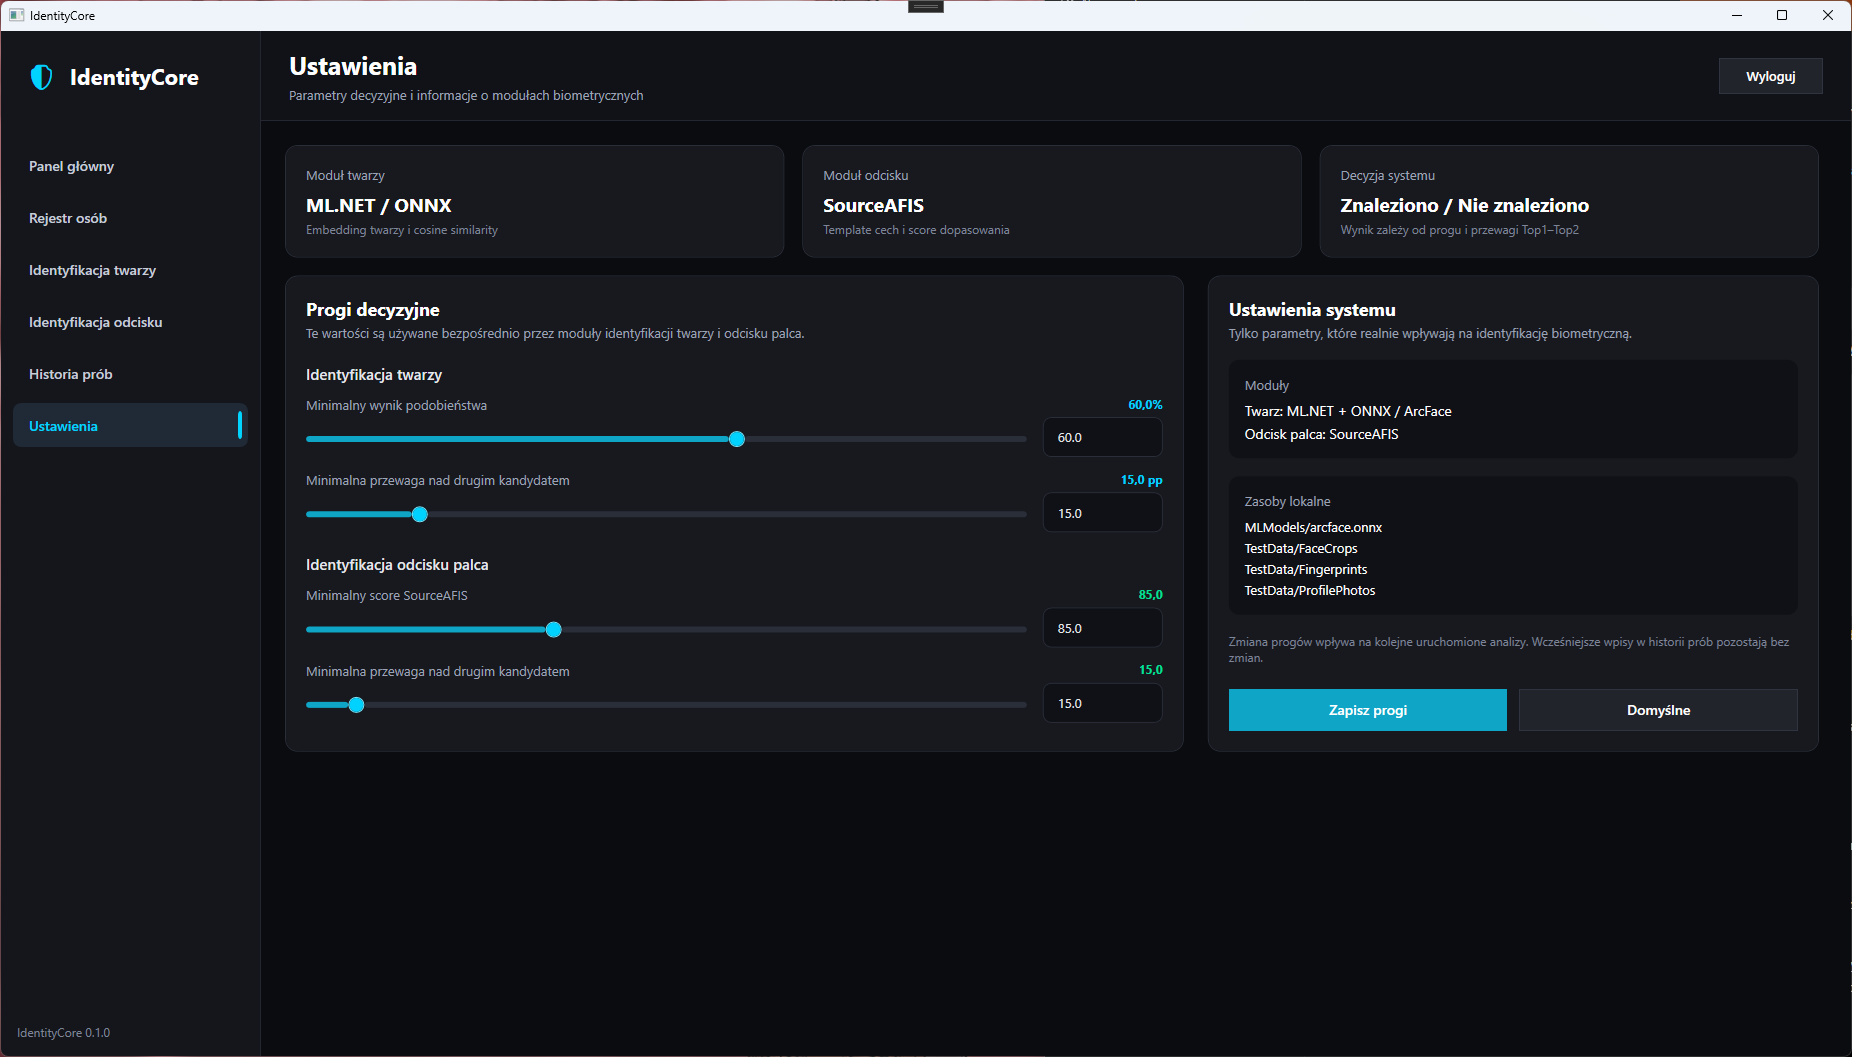
\includegraphics[width=0.98\textwidth]{figures/ui/ui_10_settings.png}
    \caption{Widok ustawień parametrów systemu}
    \label{fig:ui-settings}
\end{figure}

\section{Komunikaty i informacje zwrotne dla operatora}

Aplikacja przekazuje operatorowi informacje zwrotne bez konieczności otwierania osobnych okien dla każdego etapu pracy. W widokach identyfikacji widoczne są statusy etapów analizy, paski postępu, informacje o oczekiwaniu na wykonanie operacji oraz komunikaty o braku wyniku. Operator może więc kontrolować, czy dane wejściowe zostały wczytane, czy analiza została uruchomiona i czy system zakończył proces decyzją.

Wyniki pracy systemu są prezentowane w wydzielonych panelach. W zależności od modułu operator widzi najlepsze dopasowanie, identyfikator osoby, dział, wynik podobieństwa lub punktację, decyzję systemu oraz możliwość otwarcia profilu osoby lub zapisania próby. Historia prób pozwala natomiast wrócić do wcześniejszych zdarzeń i sprawdzić ich szczegóły. Wspólną cechą interfejsu jest wyraźne oddzielenie danych wejściowych, przebiegu analizy i rezultatu, co porządkuje sposób korzystania z aplikacji.
\chapter{Wyniki, testy i analiza skuteczności}
\label{chap:testy-analiza}

\section{Opis przygotowanych testów}

Testy aplikacji \textit{IdentityCore} miały sprawdzić praktyczne działanie dwóch modułów biometrycznych: identyfikacji twarzy oraz identyfikacji odcisku palca. Zależało przede wszystkim na potwierdzeniu, czy system poprawnie zachowuje się w dwóch podstawowych sytuacjach: gdy próbka należy do osoby zapisanej w bazie oraz gdy próbka nie powinna zostać zaakceptowana jako dopasowanie.

Dla obu modalności przygotowano po dwa przypadki testowe. Pierwszy był przypadkiem pozytywnym, w którym oczekiwano znalezienia dopasowania do osoby zarejestrowanej w systemie. Drugi był przypadkiem negatywnym, w którym system powinien zwrócić brak dopasowania. W ten sposób możliwe było sprawdzenie nie tylko samego mechanizmu rozpoznawania, ale również działania progów decyzyjnych, sposobu prezentacji wyniku oraz zgodności zaprezentowanej decyzji z rzeczywistą sytuacją testową.

Próby nie miały charakteru szerokiej walidacji statystycznej. Ich celem było sprawdzenie, czy przygotowany prototyp działa zgodnie z założeniami projektowymi i czy oba moduły biometryczne potrafią zarówno wskazać poprawnego kandydata, jak i odrzucić próbkę niespełniającą warunków akceptacji.

\section{Dane testowe}

Do badań wykorzystano cztery próby: dwie dotyczące twarzy oraz dwie dotyczące odcisku palca. Zestaw został dobrany w sposób prosty, ale celowy: dla każdej modalności uwzględniono jedną próbkę, dla której system powinien znaleźć dopasowanie, oraz jedną próbkę, dla której powinien zwrócić brak dopasowania. Dane testowe zestawiono w tabeli~\ref{tab:dane-testowe}.

\renewcommand{\arraystretch}{1.15}
\begin{xltabular}{\textwidth}{|
    >{\RaggedRight\arraybackslash}p{0.8cm}|
    >{\RaggedRight\arraybackslash}p{1.9cm}|
    >{\RaggedRight\arraybackslash}p{1.9cm}|
    >{\RaggedRight\arraybackslash}p{2.9cm}|
    >{\RaggedRight\arraybackslash}X|}

    \hline
    \textbf{Id} & \textbf{Biometria} & \textbf{Plik / źródło} & \textbf{Osoba oczekiwana} & \textbf{Charakter próbki} \\
    \hline
    \endfirsthead

    T1 & Twarz & kamera & Konrad Fugiel & Próbka twarzy osoby zapisanej w bazie, dla której oczekiwano poprawnego dopasowania. \\
    \hline
    T2 & Twarz & kamera & Brak dopasowania & Próbka twarzy osoby niewystępującej w bazie, przygotowana w celu sprawdzenia poprawnego odrzucenia. \\
    \hline
    O1 & Odcisk palca & plik & Filip Lisowski & Próbka odcisku palca osoby zapisanej w bazie, dla której oczekiwano poprawnego dopasowania. \\
    \hline
    O2 & Odcisk palca & plik & Brak dopasowania & Próbka odcisku palca, dla której system nie powinien znaleźć osoby w bazie. \\
    \hline

    \caption{Zestaw danych testowych wykorzystanych podczas oceny działania systemu}
    \label{tab:dane-testowe}
\end{xltabular}

Przygotowany zestaw jest niewielki, dlatego nie stanowi podstawy do wyznaczania miar statystycznych charakterystycznych dla pełnych badań biometrycznych. Pozwala jednak ocenić, czy system działa poprawnie w podstawowych, kontrolowanych scenariuszach pozytywnych i negatywnych.

\section{Wyniki działania systemu}

Wyniki działania systemu przedstawiono osobno dla identyfikacji twarzy i identyfikacji odcisku palca. Dla obu modułów zestawiono rezultat oczekiwany z rezultatem zwróconym przez aplikację, a następnie pokazano odpowiadające im zrzuty ekranu z wykonanych prób.

\subsection{Wyniki identyfikacji twarzy}

W module identyfikacji twarzy wykonano dwa testy. Pierwszy dotyczył osoby zapisanej w bazie i zakończył się poprawnym dopasowaniem. Drugi test dotyczył osoby niewystępującej w systemie i zakończył się brakiem dopasowania. Zestawienie wyników przedstawiono w tabeli~\ref{tab:wyniki-twarz}.

\renewcommand{\arraystretch}{1.15}
\begin{xltabular}{\textwidth}{|
    >{\RaggedRight\arraybackslash}p{0.8cm}|
    >{\RaggedRight\arraybackslash}p{2.8cm}|
    >{\RaggedRight\arraybackslash}p{3.3cm}|
    >{\RaggedRight\arraybackslash}p{2.2cm}|
    >{\RaggedRight\arraybackslash}X|}

    \hline
    \textbf{Id} & \textbf{Oczekiwany wynik} & \textbf{Wynik systemu} & \textbf{Wynik dopasowania} & \textbf{Ocena} \\
    \hline
    \endfirsthead

    \hline
    \textbf{Id} & \textbf{Oczekiwany wynik} & \textbf{Wynik systemu} & \textbf{Wynik dopasowania} & \textbf{Ocena} \\
    \hline
    \endhead

    T1 & Konrad Fugiel & Znaleziono dopasowanie: Konrad Fugiel & 84,2\% & Poprawne dopasowanie. Wynik przekroczył próg 60,0\%. \\
    \hline
    T2 & Brak dopasowania & Nie znaleziono osoby w bazie & 41,4\% & Brak dopasowania zgodny z oczekiwaniem. Wynik był poniżej progu 60,0\%. \\
    \hline

    \caption{Wyniki testów identyfikacji twarzy}
    \label{tab:wyniki-twarz}
\end{xltabular}

Pierwsza próba twarzy zakończyła się poprawnym rozpoznaniem osoby zapisanej w bazie. System wskazał osobę \textit{Konrad Fugiel}, a wynik podobieństwa osiągnął wartość \(84{,}2\%\). W prawym panelu widoku wynikowego widoczna jest zarówno decyzja \textit{Znaleziono dopasowanie}, jak i szczegóły najlepszego kandydata. Dla tej próby nie pojawił się drugi kandydat, dlatego decyzja została oparta na jednoznacznym najlepszym wyniku.

\begin{figure}[H]
    \centering
    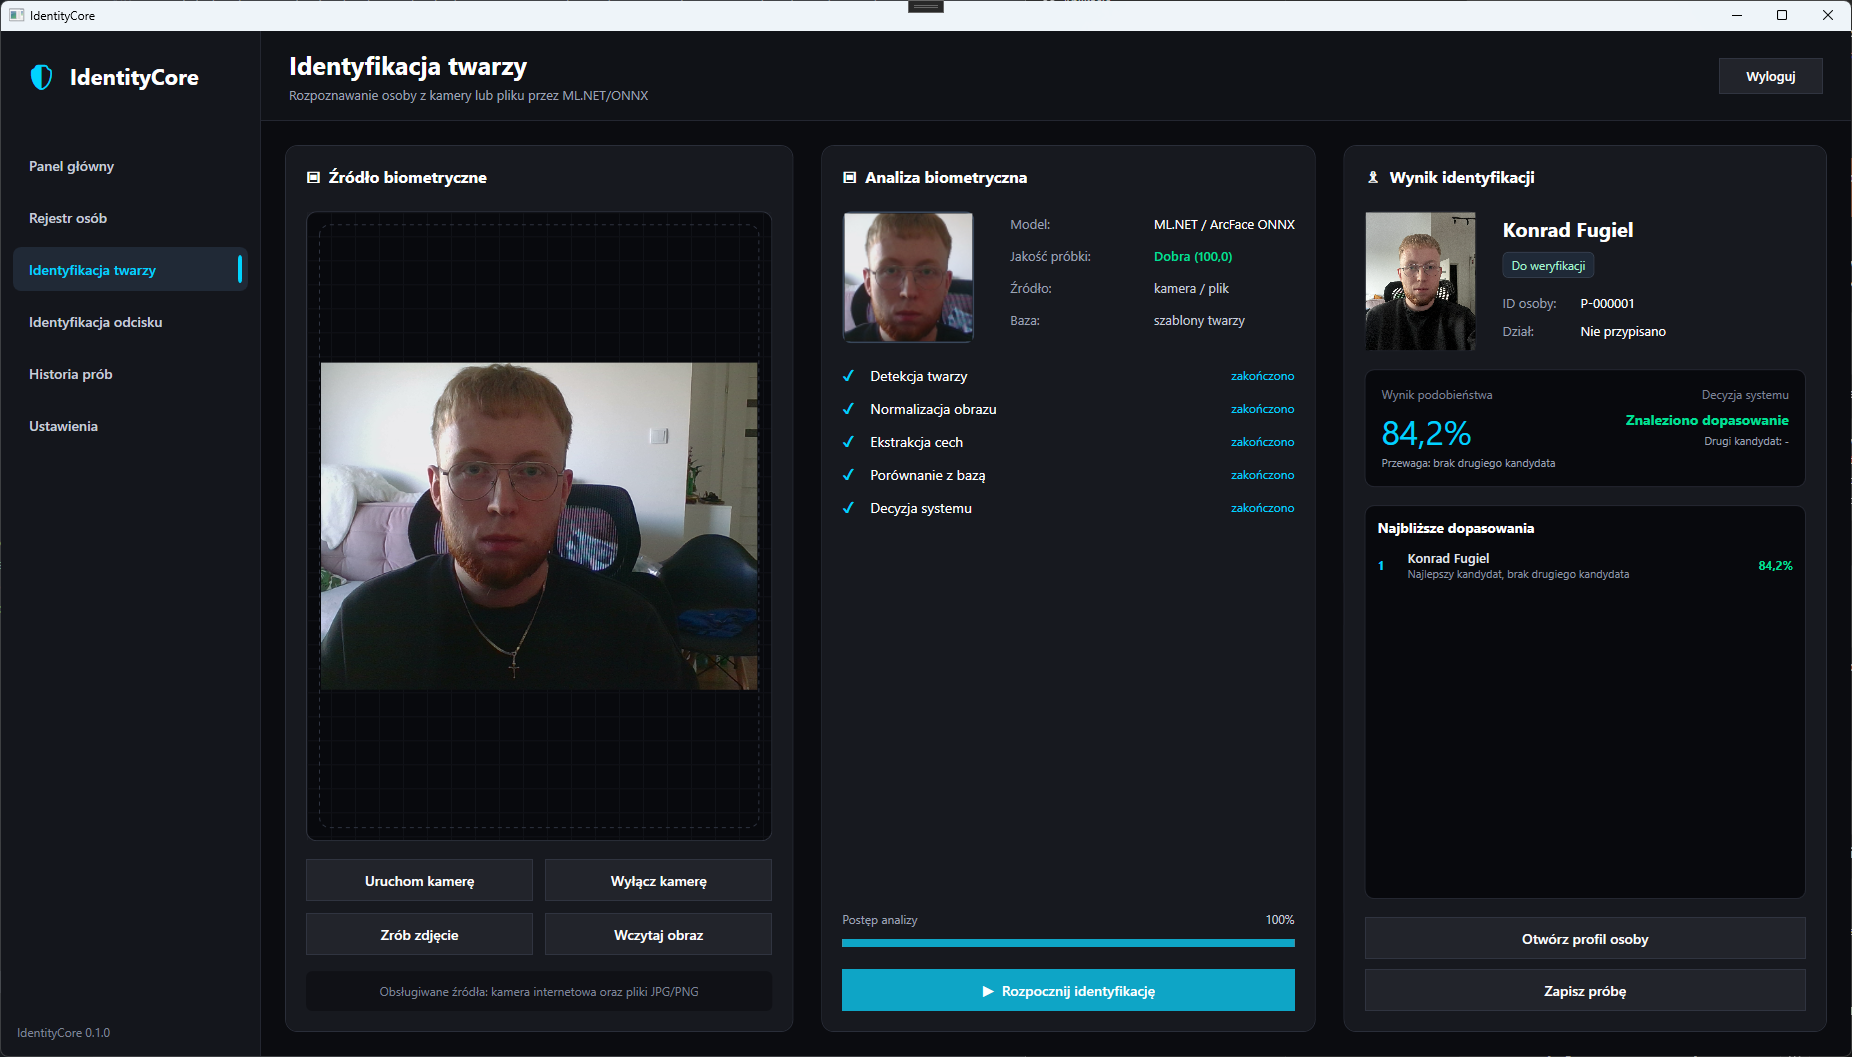
\includegraphics[width=0.98\textwidth]{figures/results/result_01_face_match.png}
    \caption{Wynik pozytywnej identyfikacji twarzy}
    \label{fig:result-face-match}
\end{figure}

Druga próba twarzy miała charakter negatywny. Do systemu wprowadzono twarz osoby niewystępującej w bazie, dlatego oczekiwano odrzucenia wyniku. System rzeczywiście nie zaakceptował dopasowania i zwrócił komunikat \textit{Nie znaleziono osoby w bazie}. Najlepszy uzyskany wynik wyniósł \(41{,}4\%\), co było wartością niższą od ustawionego progu \(60{,}0\%\). W widoku wynikowym pokazano również najbliższe dopasowanie, jednak nie zostało ono zaakceptowane jako rozpoznanie.

\begin{figure}[H]
    \centering
    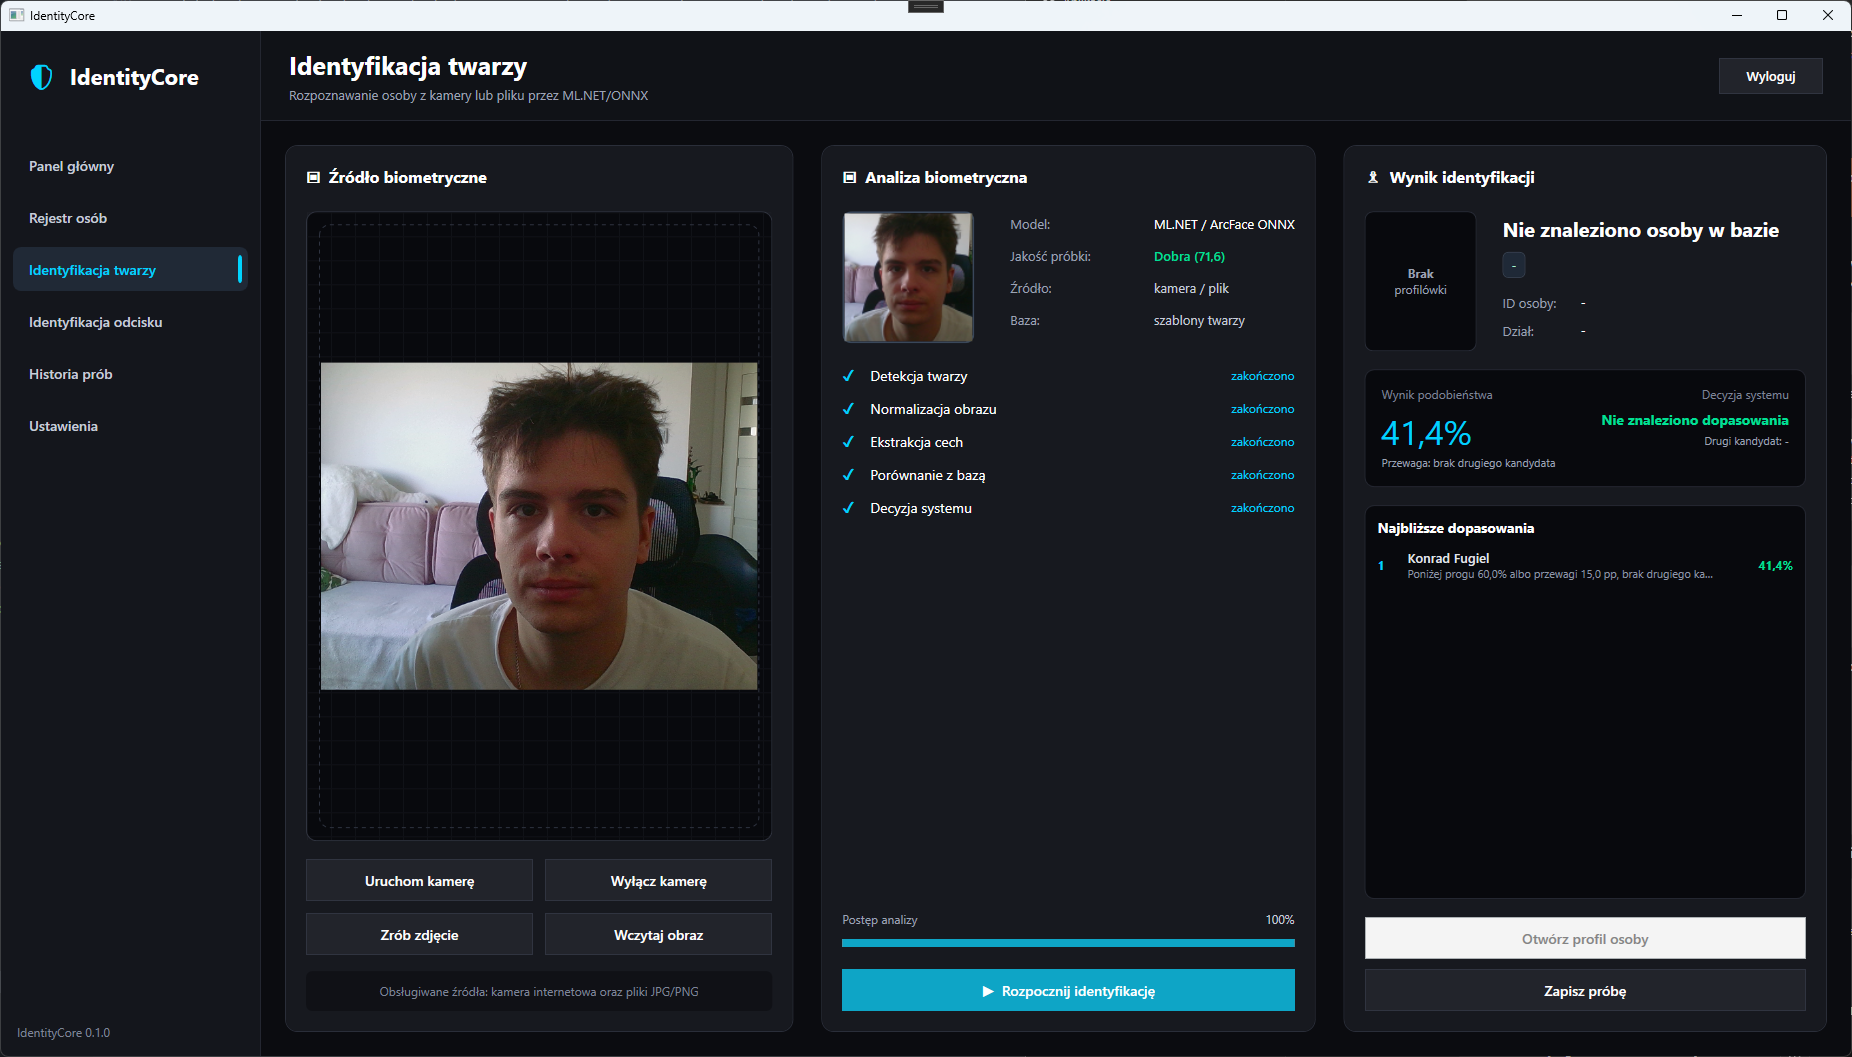
\includegraphics[width=0.98\textwidth]{figures/results/result_02_face_no_match.png}
    \caption{Wynik negatywnej identyfikacji twarzy}
    \label{fig:result-face-no-match}
\end{figure}

\subsection{Wyniki identyfikacji odcisku palca}

W module identyfikacji odcisku palca również przeprowadzono dwa testy: jeden pozytywny oraz jeden negatywny. W pierwszym przypadku system powinien wskazać osobę zapisaną w bazie, a w drugim zwrócić brak dopasowania. Wyniki zestawiono w tabeli~\ref{tab:wyniki-odcisk}.

\renewcommand{\arraystretch}{1.15}
\begin{xltabular}{\textwidth}{|
    >{\RaggedRight\arraybackslash}p{0.8cm}|
    >{\RaggedRight\arraybackslash}p{2.8cm}|
    >{\RaggedRight\arraybackslash}p{3.3cm}|
    >{\RaggedRight\arraybackslash}p{2.2cm}|
    >{\RaggedRight\arraybackslash}X|}

    \hline
    \textbf{Id} & \textbf{Oczekiwany wynik} & \textbf{Wynik systemu} & \textbf{Score dopasowania} & \textbf{Ocena} \\
    \hline
    \endfirsthead

    \hline
    \textbf{Id} & \textbf{Oczekiwany wynik} & \textbf{Wynik systemu} & \textbf{Score dopasowania} & \textbf{Ocena} \\
    \hline
    \endhead

    O1 & Filip Lisowski & Znaleziono dopasowanie: Filip Lisowski & 190,4 & Poprawne dopasowanie. Wynik znacząco przekroczył próg 85,0. \\
    \hline
    O2 & Brak dopasowania & Nie znaleziono osoby w bazie & 9,6 & Brak dopasowania zgodny z oczekiwaniem. Wynik był poniżej progu 85,0. \\
    \hline

    \caption{Wyniki testów identyfikacji odcisku palca}
    \label{tab:wyniki-odcisk}
\end{xltabular}

\newpage

Pozytywna próba odcisku palca została wykonana dla pliku graficznego. System wskazał osobę \textit{Filip Lisowski}, a wynik dopasowania wyniósł \(190{,}4\), czyli wyraźnie przekroczył próg \(85{,}0\). Widok wynikowy pokazuje nie tylko decyzję \textit{Znaleziono dopasowanie}, ale również identyfikator osoby oraz przewagę najlepszego wyniku nad kolejnym kandydatem.

\begin{figure}[H]
    \centering
    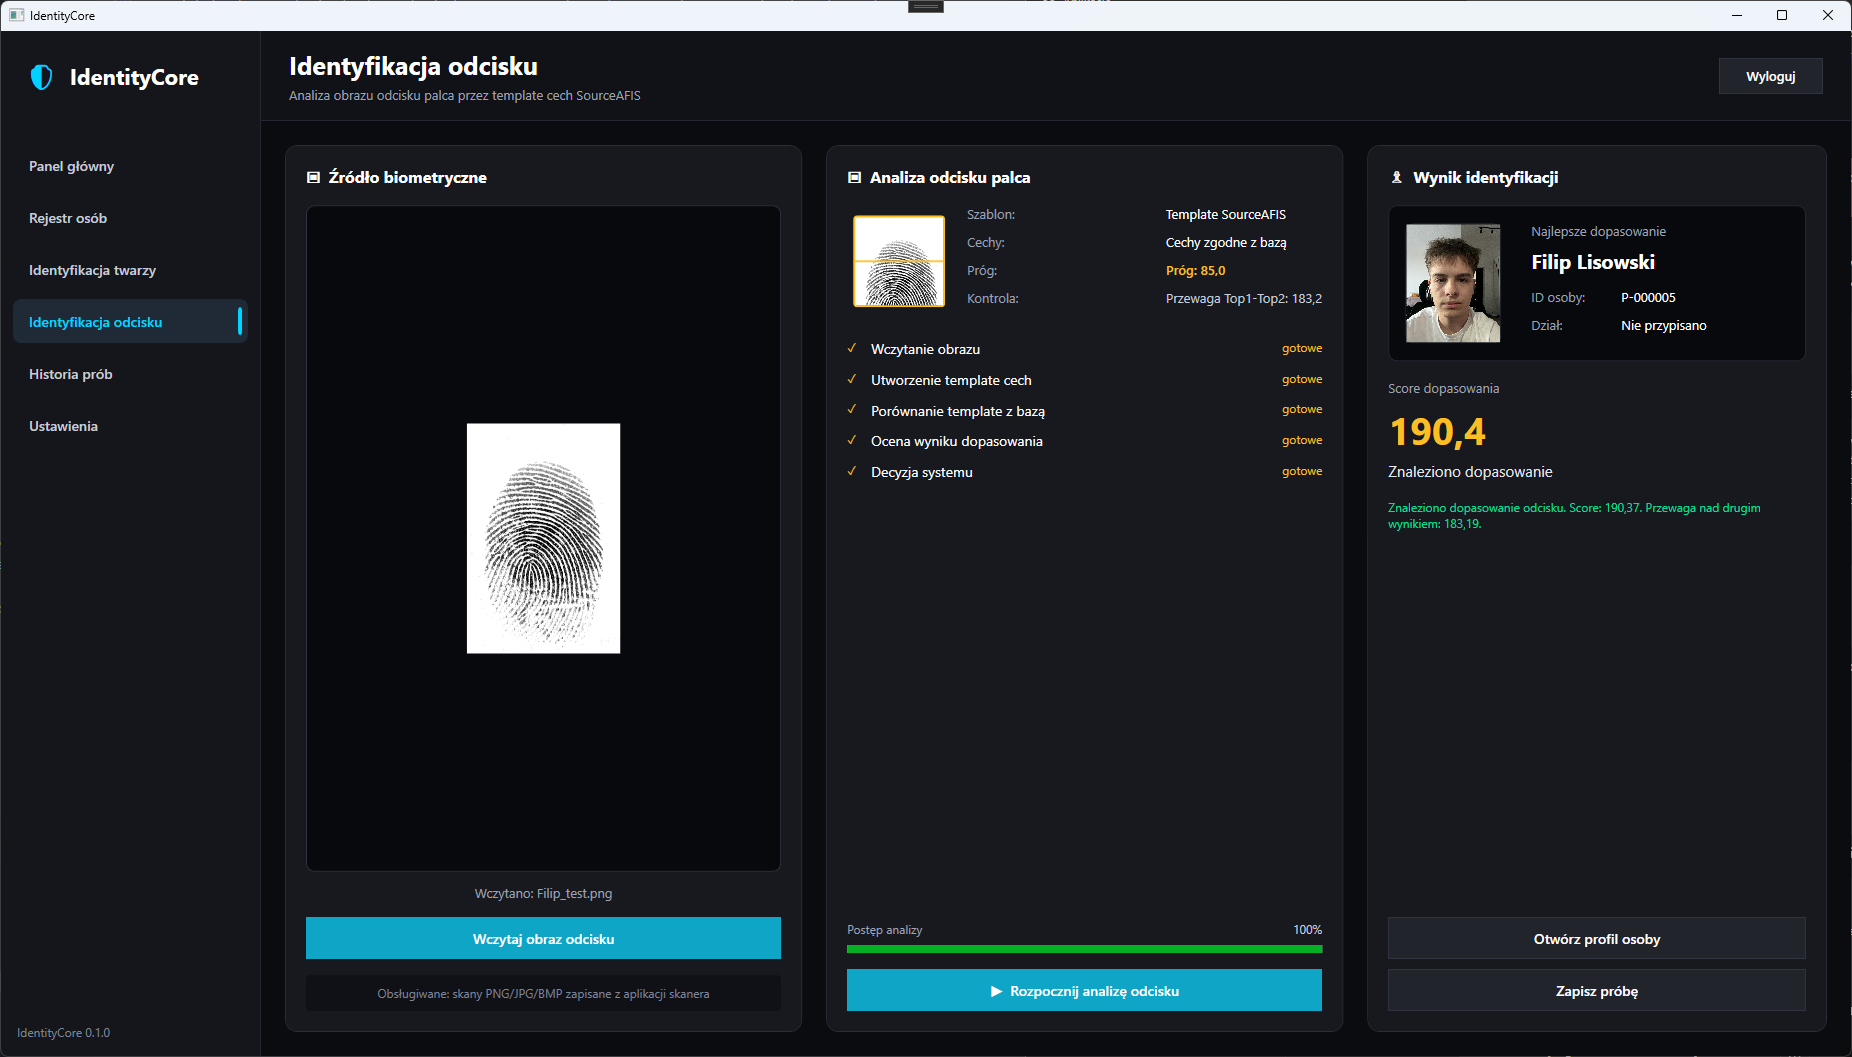
\includegraphics[width=0.98\textwidth]{figures/results/result_03_fingerprint_match.png}
    \caption{Wynik pozytywnej identyfikacji odcisku palca}
    \label{fig:result-fingerprint-match}
\end{figure}

Negatywna próba odcisku palca została wykonana dla pliku \texttt{Konrad\_test\_srodkowy.png}. W tym przypadku system nie znalazł osoby w bazie. Najwyższy uzyskany wynik wyniósł \(9{,}6\), a więc był zdecydowanie niższy od progu \(85{,}0\). Na ekranie widoczna jest również przewaga Top1--Top2 równa \(5{,}7\), jednak już sam bardzo niski wynik dopasowania był wystarczający do odrzucenia próby.

\begin{figure}[H]
    \centering
    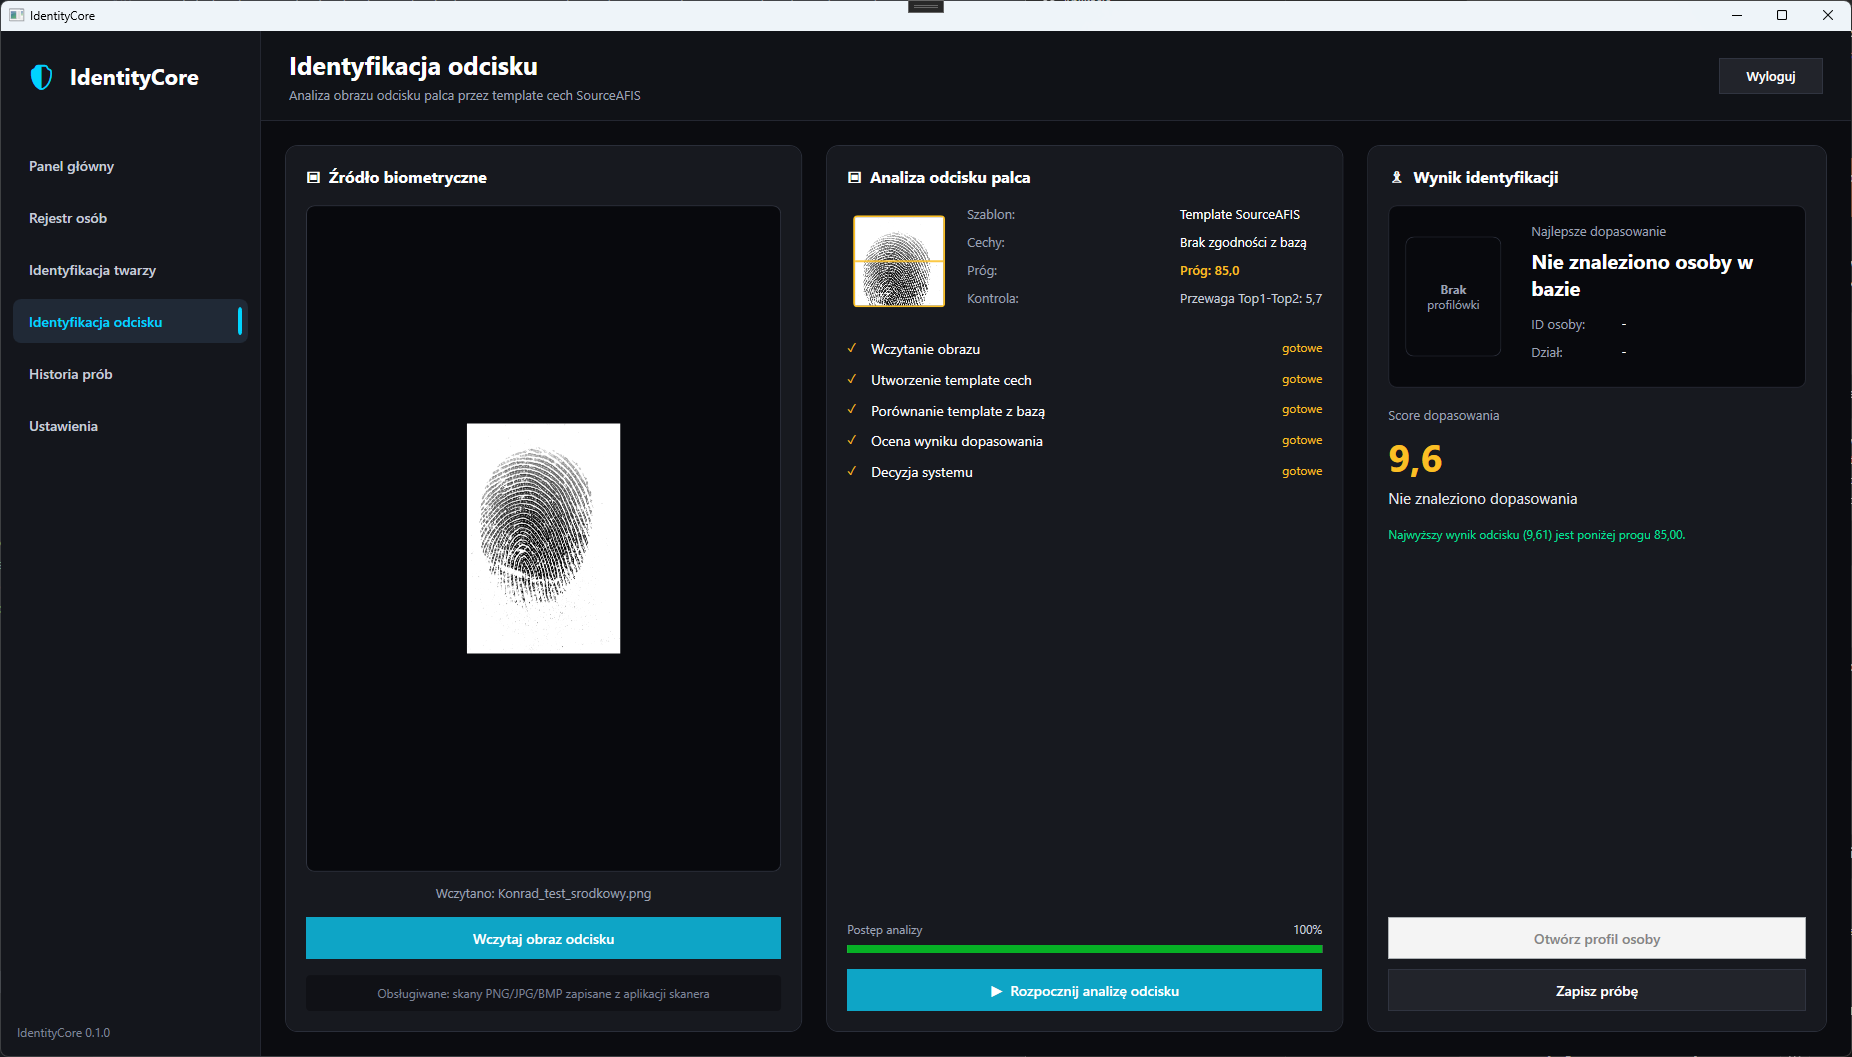
\includegraphics[width=0.98\textwidth]{figures/results/result_04_fingerprint_no_match.png}
    \caption{Wynik negatywnej identyfikacji odcisku palca}
    \label{fig:result-fingerprint-no-match}
\end{figure}

\section{Analiza poprawnych i błędnych rozpoznań}

W przeprowadzonym zestawie testowym wystąpiły zarówno przypadki poprawnego dopasowania, jak i poprawnego braku dopasowania. Dla twarzy system prawidłowo rozpoznał osobę \textit{Konrad Fugiel} przy wyniku \(84{,}2\%\) oraz prawidłowo odrzucił próbkę osoby niewystępującej w bazie przy wyniku \(41{,}4\%\). Dla odcisku palca system poprawnie wskazał osobę \textit{Filip Lisowski} przy wyniku \(190{,}4\) oraz poprawnie odrzucił próbkę negatywną z wynikiem \(9{,}6\).

W badanym zestawie nie wystąpił ani błędny brak dopasowania, ani błędne przypisanie próbki do niewłaściwej osoby. Wystąpiły natomiast dwa przypadki braku dopasowania i w obu sytuacjach był to rezultat zgodny z oczekiwaniem. Oznacza to, że w przygotowanych warunkach testowych system nie tylko znajdował poprawne dopasowania, ale potrafił również odrzucać próbki, które nie powinny zostać zaakceptowane.

Trzeba jednak podkreślić, że wnioski te dotyczą wyłącznie małego zestawu testowego. Wyniki mają charakter poglądowy i pokazują zachowanie prototypu w kilku kontrolowanych przypadkach, a nie pełną ocenę skuteczności systemu biometrycznego.

\section{Wpływ parametrów na działanie systemu}

W aplikacji zastosowano cztery główne parametry decyzyjne: dla twarzy próg podobieństwa \(60{,}0\%\) i margines \(15{,}0\) pp, a dla odcisku palca próg \(85{,}0\) i margines \(15{,}0\). W wykonanych próbach pozytywne przypadki przekroczyły wymagane progi, natomiast obie próby negatywne zostały odrzucone, ponieważ uzyskane wyniki były zbyt niskie.

W praktyce obniżenie progów mogłoby zwiększyć liczbę zaakceptowanych dopasowań, ale jednocześnie podniosłoby ryzyko błędnej akceptacji. Z kolei podwyższenie progów mogłoby poprawić ostrożność decyzji, ale kosztem częstszego odrzucania nawet poprawnych próbek. Dodatkową rolę pełni margines Top1--Top2, który pomaga odrzucać przypadki niejednoznaczne. Zmiana tych ustawień wpływa wyłącznie na kolejne próby i nie modyfikuje wcześniej zapisanych wyników w historii.

\section{Wnioski z eksperymentów}

Przeprowadzone testy potwierdziły, że aplikacja \textit{IdentityCore} realizuje podstawowy cel demonstracyjny. Oba moduły biometryczne potrafiły poprawnie wskazać osobę zapisaną w bazie oraz zwrócić brak dopasowania w sytuacji, gdy próbka nie powinna zostać zaakceptowana.

Najważniejszym ograniczeniem badań jest mała liczba prób. Aby rzetelniej ocenić skuteczność systemu, należałoby przygotować większy i bardziej zróżnicowany zbiór danych, obejmujący więcej osób, więcej przypadków negatywnych oraz próbki o różnej jakości. Na obecnym etapie wyniki należy więc traktować jako potwierdzenie poprawnego działania prototypu, a nie jako pełną walidację skuteczności rozwiązania.
\chapter{Analiza bezpieczeństwa systemu}
\label{chap:bezpieczenstwo}

\section{Potencjalne zagrożenia}

System \textit{IdentityCore} jest lokalną aplikacją demonstracyjną, dlatego główne zagrożenia dotyczą przede wszystkim danych wejściowych, lokalnej bazy oraz konfiguracji parametrów decyzyjnych. Operator może wczytywać obrazy z plików, co oznacza, że jako dane wejściowe mogą zostać podane wcześniej przygotowane lub zmodyfikowane obrazy twarzy i odcisków palców. Ryzyko dotyczy więc nie tylko jakości próbki, ale również możliwości podstawienia danych niepochodzących bezpośrednio od badanej osoby.

Drugim obszarem ryzyka jest lokalna baza danych, w której przechowywane są informacje o osobach, szablony biometryczne, ustawienia i historia prób. Podmiana, uszkodzenie lub nieuprawniona modyfikacja tych danych mogłaby wpłynąć na działanie systemu. Znaczenie mają również progi decyzyjne: zbyt niskie wartości mogą zwiększać ryzyko błędnej akceptacji, a zbyt wysokie mogą powodować częstsze odrzucanie poprawnych próbek.

\section{Ryzyko fałszowania danych biometrycznych}

Istotnym ograniczeniem prototypu jest brak pełnego mechanizmu wykrywania żywotności próbki, czyli \textit{liveness detection}. Oznacza to, że system może być podatny na próby użycia zdjęcia twarzy zamiast żywej osoby, obrazu twarzy wyświetlonego na ekranie albo wcześniej przygotowanego pliku graficznego. Podobne ryzyko dotyczy odcisków palców, gdzie do aplikacji można wprowadzić skan lub kopię odcisku zapisaną jako obraz.

W obecnej wersji aplikacja analizuje dostarczony obraz i podejmuje decyzję na podstawie wyniku dopasowania, progu oraz marginesu. Nie sprawdza jednak w zaawansowany sposób, czy próbka pochodzi od osoby obecnej fizycznie przy stanowisku.

\section{Błędy identyfikacji}

W systemach biometrycznych mogą wystąpić dwa podstawowe typy błędów: fałszywa akceptacja oraz fałszywe odrzucenie. Fałszywa akceptacja oznacza uznanie próbki za zgodną z osobą z bazy mimo braku rzeczywistej zgodności. Fałszywe odrzucenie oznacza brak dopasowania mimo tego, że próbka pochodzi od osoby zapisanej w systemie.

Na decyzję wpływa jakość danych wejściowych. W przypadku twarzy znaczenie mają oświetlenie, ostrość, ustawienie głowy i widoczność twarzy. W przypadku odcisku palca istotne są czytelność linii papilarnych, kompletność próbki, kontrast i ewentualne rozmazanie. Dodatkowym zabezpieczeniem jest margines między najlepszym i drugim kandydatem, który ogranicza akceptację przypadków niejednoznacznych.

\section{Ocena odporności systemu}

Aplikacja posiada podstawowe mechanizmy ograniczające ryzyko błędnej decyzji. Należą do nich progi decyzyjne, margines Top1--Top2, odrzucanie wyników poniżej progu, komunikaty o nieudanej analizie oraz historia prób identyfikacji.

Jednocześnie odporność systemu jest ograniczona. Prototyp nie posiada pełnego wykrywania żywotności próbki, nie zawiera rozbudowanego modelu ról użytkowników i nie powinien być traktowany jako system produkcyjnie bezpieczny.

\section{Możliwe usprawnienia bezpieczeństwa}

Najważniejszym kierunkiem rozwoju byłoby dodanie mechanizmów \textit{liveness detection} dla identyfikacji twarzy, aby ograniczyć ryzyko użycia zdjęcia lub obrazu wyświetlonego na ekranie. W module odcisku palca warto rozważyć bezpośrednią integrację ze skanerem, zamiast opierania procesu wyłącznie na wczytywaniu plików graficznych.

Kolejne usprawnienia powinny dotyczyć ochrony danych i dostępu do aplikacji. W przyszłości warto dodać hashowanie i solenie haseł operatora, blokadę po wielu błędnych próbach logowania, szyfrowanie szablonów biometrycznych oraz dokładniejsze rejestrowanie zdarzeń administracyjnych. Dodatkowo system powinien zostać sprawdzony na większym zbiorze danych, z uwzględnieniem testów fałszywej akceptacji i fałszywego odrzucenia.
\chapter{Harmonogram realizacji projektu}
\label{chap:harmonogram}

\section{Etapy realizacji}

Prace nad projektem \textit{IdentityCore} rozpoczęto na początku maja 2026 roku, a zakończono w drugim tygodniu czerwca 2026 roku. Projekt był realizowany etapowo, jednak poszczególne części częściowo nakładały się na siebie. Wynikało to z charakteru aplikacji, w której warstwa interfejsu, baza danych, logika biometryczna i testy musiały być rozwijane równolegle.

Pierwszym etapem było określenie zakresu projektu oraz wybór głównych funkcji systemu. Ustalono, że aplikacja będzie lokalnym systemem identyfikacji osób, wykorzystującym dwa typy danych biometrycznych: obraz twarzy oraz obraz odcisku palca. Na tym etapie doprecyzowano również, że projekt będzie aplikacją desktopową z bazą danych SQL Server.

Kolejne etapy obejmowały przygotowanie struktury aplikacji, modelu danych oraz widoków WPF. Następnie rozwijano rejestr osób, obsługę profilu osoby, zapisywanie zdjęcia profilowego oraz powiązanie osoby z próbkami biometrycznymi. Po przygotowaniu podstaw aplikacji rozpoczęto implementację modułów identyfikacji twarzy i odcisku palca.

W końcowej części prac skupiono się na dopracowaniu interfejsu, historii prób, ustawieniach systemowych, testach oraz dokumentacji. Ostatni etap obejmował poprawki, uporządkowanie plików SQL, przygotowanie zrzutów ekranu i opis działania systemu w pracy projektowej.

\section{Harmonogram prac}

Harmonogram prac został przygotowany w ujęciu tygodniowym. Daty mają charakter porządkujący i odzwierciedlają główne etapy pracy nad aplikacją.

\renewcommand{\arraystretch}{1.15}
\begin{xltabular}{\textwidth}{|
    >{\RaggedRight\arraybackslash}p{1.2cm}|
    >{\RaggedRight\arraybackslash}p{3.2cm}|
    >{\RaggedRight\arraybackslash}p{2.6cm}|
    >{\RaggedRight\arraybackslash}X|}

    \hline
    \textbf{Etap} & \textbf{Zakres prac} & \textbf{Termin} & \textbf{Rezultat} \\
    \hline
    \endfirsthead

    \hline
    \textbf{Etap} & \textbf{Zakres prac} & \textbf{Termin} & \textbf{Rezultat} \\
    \hline
    \endhead

    1 & Analiza założeń i zakresu projektu & 04.05--08.05.2026 & Ustalenie zakresu funkcji oraz głównych modułów aplikacji. \\
    \hline
    2 & Przygotowanie struktury projektu i bazy danych & 09.05--15.05.2026 & Utworzenie podstaw aplikacji, struktury katalogów, modelu danych i skryptów SQL. \\
    \hline
    3 & Rejestr osób i profil osoby & 16.05--22.05.2026 & Przygotowanie obsługi osób, edycji profilu, zdjęcia profilowego oraz próbek biometrycznych. \\
    \hline
    4 & Moduł identyfikacji twarzy & 23.05--29.05.2026 & Dodanie obsługi obrazu twarzy, modelu \texttt{arcface.onnx}, porównywania embeddingów i decyzji systemu. \\
    \hline
    5 & Moduł identyfikacji odcisku palca & 27.05--02.06.2026 & Dodanie obsługi obrazów odcisków, szablonów SourceAFIS, porównywania wzorców i decyzji systemu. \\
    \hline
    6 & Historia, ustawienia i panel główny & 03.06--07.06.2026 & Przygotowanie historii prób, parametrów decyzyjnych, podsumowań systemu i szybkich przejść. \\
    \hline
    7 & Testy, poprawki i finalizacja aplikacji & 08.06--11.06.2026 & Sprawdzenie działania modułów, korekty błędów, przygotowanie danych testowych i zrzutów ekranu. \\
    \hline
    8 & Dokumentacja projektu & 10.06--14.06.2026 & Przygotowanie opisu projektu, rozdziałów dokumentacji, wyników testów i materiałów końcowych. \\
    \hline

    \caption{Harmonogram realizacji projektu IdentityCore}
    \label{tab:harmonogram-prac}
\end{xltabular}

\section{Podział pracy}

Projekt był realizowany zespołowo. Prace nie zostały sztywno podzielone na całkowicie oddzielne części wykonywane niezależnie przez poszczególne osoby. Zespół pracował wspólnie nad najważniejszymi decyzjami projektowymi, zakresem funkcji, wyglądem aplikacji, testami oraz dokumentacją.

Wspólny charakter pracy był szczególnie istotny przy modułach biometrycznych, ponieważ identyfikacja twarzy, identyfikacja odcisku palca, rejestr osób i historia prób są ze sobą powiązane. Zmiana w jednym module często wymagała sprawdzenia działania pozostałych elementów aplikacji. Z tego powodu wiele zadań było konsultowanych i testowanych wspólnie.

W praktyce praca zespołu obejmowała wspólne ustalanie wymagań, projektowanie struktury aplikacji, przygotowywanie widoków, implementację funkcji, testowanie działania systemu oraz opracowanie dokumentacji. Taki sposób pracy pozwolił zachować spójność projektu i uniknąć sytuacji, w której poszczególne moduły działałyby osobno, ale nie tworzyłyby jednego kompletnego systemu.
\chapter{Instrukcja uruchomienia projektu}
\label{chap:instrukcja-uruchomienia}

\section{Wymagania systemowe}

Do uruchomienia aplikacji \textit{IdentityCore} wymagane jest lokalne stanowisko z systemem Windows oraz środowiskiem umożliwiającym kompilację aplikacji desktopowej WPF/.NET. Projekt był przygotowywany i uruchamiany w środowisku Visual Studio 2026 w wersji 18.5.2, z projektem docelowym ustawionym na \texttt{net10.0-windows}.

Aplikacja korzysta również z lokalnej bazy danych SQL Server oraz modelu \texttt{arcface.onnx}, który jest przechowywany w projekcie jako plik zarządzany przez Git LFS. Z tego powodu samo pobranie repozytorium nie jest wystarczające, jeżeli pliki LFS nie zostaną pobrane poprawnie.

\renewcommand{\arraystretch}{1.15}
\begin{xltabular}{\textwidth}{|
    >{\RaggedRight\arraybackslash}p{4.5cm}|
    >{\RaggedRight\arraybackslash}X|}

    \hline
    \textbf{Element} & \textbf{Wymaganie} \\
    \hline
    \endfirsthead

    \hline
    \textbf{Element} & \textbf{Wymaganie} \\
    \hline
    \endhead

    System operacyjny & Windows z obsługą aplikacji desktopowych .NET/WPF. \\
    \hline
    Środowisko programistyczne & Visual Studio 2026, wersja 18.5.2. \\
    \hline
    Platforma .NET & .NET 10, projekt docelowy \texttt{net10.0-windows}. \\
    \hline
    Baza danych & SQL Server oraz SQL Server Management Studio. \\
    \hline
    Repozytorium & Git oraz Git LFS do pobrania kodu i dużych plików projektu. \\
    \hline
    Model twarzy & Plik \texttt{IdentityCore.App/MLModels/arcface.onnx}. \\
    \hline

    \caption{Podstawowe wymagania potrzebne do uruchomienia projektu}
    \label{tab:wymagania-uruchomieniowe}
\end{xltabular}

\section{Konfiguracja środowiska}

Pierwszym krokiem jest pobranie projektu z repozytorium. Ponieważ projekt wykorzystuje plik modelu \texttt{arcface.onnx}, należy upewnić się, że na stanowisku zainstalowany jest Git LFS. Po sklonowaniu repozytorium trzeba pobrać pliki zarządzane przez LFS.

\begin{lstlisting}[language=bash, caption={Przykładowe pobranie projektu i plików Git LFS}, label={lst:git-lfs-pobranie}]
git clone https://github.com/KonradF20/IdentityCore.git
cd IdentityCore
git lfs pull
\end{lstlisting}

Po wykonaniu tych poleceń należy sprawdzić, czy w projekcie znajduje się plik \texttt{IdentityCore.App/MLModels/arcface.onnx}. Brak tego pliku uniemożliwi poprawne działanie modułu identyfikacji twarzy.

Następnie projekt należy otworzyć w Visual Studio. Po otwarciu rozwiązania środowisko powinno przywrócić pakiety NuGet automatycznie. Jeżeli tak się nie stanie, należy użyć opcji przywrócenia pakietów z poziomu Visual Studio albo wykonać polecenie \texttt{dotnet restore}. W ustawieniach projektu należy również sprawdzić, czy aplikacja jest kompilowana dla platformy \texttt{net10.0-windows}.

\section{Konfiguracja bazy danych}

Aplikacja korzysta z lokalnej bazy SQL Server. Przed uruchomieniem programu należy upewnić się, że usługa SQL Server działa, a następnie otworzyć SQL Server Management Studio i połączyć się z właściwą instancją serwera.

Do przygotowania bazy od podstaw służy skrypt \texttt{create\_database.sql}. Skrypt tworzy bazę \texttt{IdentityCoreDb}, tabele wymagane przez aplikację, relacje, indeksy oraz dane startowe potrzebne do pracy systemu. Skrypt należy uruchomić w SQL Server Management Studio.

Po wykonaniu skryptu trzeba sprawdzić, czy aplikacja łączy się z bazą danych. Jeżeli połączenie nie działa, należy dostosować connection string zapisany w projekcie do lokalnej konfiguracji SQL Server, w szczególności nazwę instancji serwera oraz nazwę bazy danych.

Po stronie osoby uruchamiającej projekt konieczne jest sprawdzenie, czy connection string wskazuje na lokalną instancję SQL Server oraz bazę \texttt{IdentityCoreDb}. W przypadku innej nazwy instancji SQL Server należy dostosować dane połączenia w projekcie do konfiguracji danego stanowiska.

\section{Uruchomienie aplikacji}

Zalecanym sposobem uruchomienia projektu jest użycie Visual Studio. Po otwarciu rozwiązania należy ustawić projekt \texttt{IdentityCore.App} jako projekt startowy, a następnie skompilować rozwiązanie. Jeżeli kompilacja zakończy się poprawnie, aplikację można uruchomić przyciskiem startowym w Visual Studio.

Po uruchomieniu powinien pojawić się ekran logowania. Po zalogowaniu operator może sprawdzić podstawowe moduły aplikacji: panel główny, rejestr osób, identyfikację twarzy, identyfikację odcisku palca, historię prób oraz ustawienia systemowe.

Projekt można również uruchomić z poziomu terminala, o ile stanowisko ma poprawnie skonfigurowane środowisko .NET i znajduje się w katalogu projektu.

\begin{lstlisting}[language=bash, caption={Przykładowe uruchomienie aplikacji z poziomu katalogu projektu}, label={lst:dotnet-run}]
dotnet restore
dotnet build
dotnet run --project IdentityCore.App
\end{lstlisting}

Jeżeli struktura katalogów w lokalnej kopii różni się od powyższego przykładu, ścieżkę po parametrze \texttt{-{}-project} należy dopasować do lokalizacji pliku \texttt{IdentityCore.App.csproj}.

\section{Dane testowe i konta testowe}

Do paczki projektu nie dołączono pełnego zestawu danych biometrycznych używanego podczas testów. Wynika to z charakteru danych przetwarzanych przez aplikację: obrazy twarzy oraz odcisków palców mogą być traktowane jako dane wrażliwe i nie powinny być udostępniane bez wyraźnej potrzeby. Testy opisane w pracy zostały wykonane na lokalnie przygotowanych próbkach zespołu.

W celu ponownego sprawdzenia działania aplikacji osoba uruchamiająca projekt powinna przygotować własne dane testowe. Dla modułu twarzy można wykorzystać obraz z kamery albo plik graficzny przedstawiający twarz. Dla modułu odcisku palca należy przygotować obraz odcisku zapisany w formacie obsługiwanym przez aplikację, na przykład PNG, JPG lub BMP. Dane powinny zostać podzielone na próbki referencyjne dodawane do profilu osoby oraz próbki wejściowe wykorzystywane później do identyfikacji.

Zalecany sposób przygotowania prostego zestawu testowego jest następujący: najpierw należy utworzyć w rejestrze osobę testową, następnie zarejestrować dla niej próbkę twarzy albo odcisku palca, a dopiero później uruchomić identyfikację na drugiej próbce tej samej osoby. Do sprawdzenia przypadku negatywnego można użyć próbki innej osoby, która nie została dodana do rejestru. Dzięki temu możliwe jest sprawdzenie zarówno dopasowania, jak i braku dopasowania.

Pliki robocze generowane lub kopiowane przez aplikację są zapisywane lokalnie w katalogu uruchomieniowym programu, czyli w strukturze tworzonej podczas kompilacji pod katalogiem \texttt{bin}. Dokładna ścieżka może zależeć od trybu uruchomienia, konfiguracji kompilacji oraz ustawień środowiska Visual Studio. Z tego powodu po pierwszym uruchomieniu aplikacji warto sprawdzić katalog wynikowy projektu \texttt{IdentityCore.App}, w szczególności podkatalogi utworzone obok pliku wykonywalnego.

Do zalogowania w środowisku demonstracyjnym wykorzystywane jest konto testowe:

\begin{lstlisting}[caption={Dane konta testowego operatora}, label={lst:konto-testowe}]
login: admin
haslo: admin
\end{lstlisting}

Po zalogowaniu można sprawdzić działanie podstawowych modułów: przejrzeć rejestr osób, dodać osobę testową, zarejestrować próbki biometryczne, uruchomić identyfikację twarzy lub odcisku palca, zapisać próbę do historii oraz sprawdzić wartości progów w ustawieniach systemu.

\chapter{Podsumowanie i wnioski końcowe}
\label{chap:podsumowanie}

\section{Ocena realizacji założeń}

Celem projektu było przygotowanie lokalnej aplikacji desktopowej umożliwiającej identyfikację osób na podstawie danych biometrycznych twarzy oraz odcisku palca. Założenie to zostało zrealizowane w postaci aplikacji \textit{IdentityCore}, która łączy rejestr osób, obsługę próbek biometrycznych, proces identyfikacji, historię prób oraz ustawienia parametrów decyzyjnych.

W projekcie udało się przygotować spójny system, w którym osoba może zostać dodana do rejestru, uzupełniona o dane profilowe i powiązana z materiałem biometrycznym. Aplikacja pozwala następnie uruchomić identyfikację twarzy lub odcisku palca, zaprezentować wynik operatorowi oraz zapisać próbę w historii. Zrealizowano również panel główny, ekran logowania, widok ustawień oraz widok historii, dzięki czemu aplikacja nie ogranicza się wyłącznie do pojedynczego algorytmu, ale tworzy pełniejszy prototyp systemu identyfikacji.

Założenia projektowe zostały więc spełnione na poziomie demonstracyjnym. System pokazuje kompletny przepływ pracy: od rejestracji osoby, przez przygotowanie danych biometrycznych, po wykonanie próby identyfikacji i zapis wyniku.

\section{Napotkane problemy}

Największe trudności dotyczyły integracji części biometrycznej z aplikacją desktopową i bazą danych. W przypadku identyfikacji twarzy istotnym problemem było poprawne przygotowanie obrazu przed przekazaniem go do modelu. Należało zadbać o wykrycie twarzy, przygotowanie odpowiedniego wycinka obrazu, wygenerowanie reprezentacji twarzy oraz porównanie jej z zapisanymi wzorcami.

W przypadku odcisków palców problemem było przygotowanie takiego sposobu pracy, który pozwalałby analizować obrazy zapisane w plikach. Ponieważ projekt nie opierał się na pełnej integracji ze skanerem linii papilarnych, konieczne było przyjęcie rozwiązania polegającego na wczytywaniu obrazów odcisków. Pozwoliło to zrealizować moduł identyfikacji, ale jednocześnie ujawniło ograniczenia prototypu.

\section{Ocena skuteczności rozwiązania}

Przeprowadzone testy pokazały, że aplikacja działa zgodnie z założeniami w podstawowych scenariuszach. System potrafił wskazać osobę zapisaną w bazie oraz odrzucić próbkę, której wynik znajdował się poniżej przyjętego progu decyzyjnego. Dotyczyło to zarówno modułu identyfikacji twarzy, jak i modułu identyfikacji odcisku palca.

Wyniki należy jednak interpretować ostrożnie. Testy miały charakter projektowy i zostały wykonane na niewielkim zbiorze danych. Nie można na ich podstawie traktować systemu jako rozwiązania produkcyjnego ani wyciągać pełnych wniosków statystycznych dotyczących skuteczności biometrycznej. Aplikacja spełnia natomiast rolę prototypu pokazującego praktyczne działanie procesu identyfikacji.

Istotne znaczenie dla skuteczności mają jakość danych wejściowych, liczba zapisanych wzorców, wartości progów decyzyjnych oraz margines między najlepszymi kandydatami. W obecnej wersji system sprawdza te warunki i potrafi odrzucić próbkę, jeżeli wynik jest zbyt niski lub nie spełnia przyjętych kryteriów.

\section{Możliwości zastosowania systemu}

\textit{IdentityCore} może służyć jako demonstracyjny system identyfikacji osób w środowisku lokalnym. Projekt dobrze pokazuje, jak można połączyć rejestr osób, dane biometryczne, bazę danych oraz aplikację desktopową w jednym narzędziu. 

Aplikacja może znaleźć zastosowanie w sytuacjach, w których potrzebne jest pokazanie zasady działania identyfikacji biometrycznej bez wdrażania pełnego systemu produkcyjnego. Przykładem może być prezentacja działania rozpoznawania twarzy, porównywania odcisków palców, zapisu historii prób oraz wpływu parametrów decyzyjnych na wynik.

Należy podkreślić, że system nie posiada pełnych mechanizmów bezpieczeństwa wymaganych w rozwiązaniach produkcyjnych, takich jak wykrywanie żywotności próbki, zaawansowana ochrona szablonów biometrycznych czy rozbudowane zarządzanie uprawnieniami.

\section{Kierunki dalszego rozwoju}

Dalszy rozwój systemu powinien obejmować przede wszystkim zwiększenie bezpieczeństwa i odporności modułów biometrycznych. W przypadku identyfikacji twarzy ważnym kierunkiem byłoby dodanie mechanizmu wykrywania żywotności próbki, aby ograniczyć ryzyko użycia zdjęcia lub obrazu wyświetlonego na ekranie. W module odcisku palca warto rozważyć bezpośrednią integrację ze skanerem, zamiast opierania procesu wyłącznie na wczytywaniu plików graficznych.

Kolejnym kierunkiem rozwoju jest rozszerzenie testów na większym i bardziej zróżnicowanym zbiorze danych. Pozwoliłoby to dokładniej ocenić zachowanie progów decyzyjnych, liczbę błędnych akceptacji oraz liczbę błędnych odrzuceń. W przyszłości można również rozbudować ochronę danych, między innymi przez szyfrowanie szablonów biometrycznych, lepsze zabezpieczenie logowania operatora oraz dokładniejsze rejestrowanie zdarzeń administracyjnych.

%------------------------------------------------------------------------------
% Bibliografia (przed spisami)
%------------------------------------------------------------------------------

\cleardoublepage
\begingroup
  \renewcommand{\emph}[1]{\textit{#1}} % wyłącz ulem na czas bibliografii
  \addcontentsline{toc}{chapter}{Bibliografia}
  \bibliographystyle{plain}
  \bibliography{bibliografia}
\endgroup
\renewcommand{\emph}[1]{\uline{#1}} % przywróć ulem (opcjonalnie)

%------------------------------------------------------------------------------
% Spisy
%------------------------------------------------------------------------------

\cleardoublepage
\addcontentsline{toc}{chapter}{Spis rysunków}
\listoffigures

\cleardoublepage
\addcontentsline{toc}{chapter}{Spis tabel}
\listoftables

\cleardoublepage
\addcontentsline{toc}{chapter}{Spis listingów}
\lstlistoflistings

%------------------------------------------------------------------------------
% Oświadczenie o samodzielności pracy
%------------------------------------------------------------------------------

\clearpage
\include{appendix/statement-A}

\end{document}
